\documentclass[12pt]{mythesis}

 % \makeglossaries
 % % \loadglsentries{glossaries_entries}
 % %%% A
 % %%% C
 % %%% D
 % %%% E
 % \newglossaryentry{EHV}{name=EHV, description={Extremely High Velocity}}
 % %%% F
 % \newglossaryentry{FoV}{name=FoV, description={Field-of-View}}
 % \newglossaryentry{FWHM}{name=FWHM, description={Full-Width Half-Maximum}}
 % %%% G
 % \newglossaryentry{GMCs}{name=GMCs, description={Giant Molecular Clouds}}
 % %%% H
 % \newglossaryentry{HST}{name=HST, description={Hubble Space Telescope}}
 % %%% I
 % \newglossaryentry{IHV}{name=IHV, description={Intermediate High Velocity}}
 % %%% K
 % %%% L
 % %%% M
 % %%% N
 % %%% O
 % %%% P
 % %%% Q
 % %%% R
 % \newglossaryentry{RA}{name=RA, description={Right Ascension}}
 % %%% S
 % \newglossaryentry{S/N}{name=S/N, description={signal-to-noise ratio}}
 % \newglossaryentry{SHV}{name=SHV, description={Standard High Velocity}}
 % %%% T
 % %%% U
 % %%% Y
 % \newglossaryentry{YSO}{name=YSO, description={Young Stellar Object}}
 % %%% Z


\title{Observing the Sun: from start to finish.}
\author{Pablo Santamarina Guerrero}
\date{\today}
\institution{%
 Instituto de Astrofísica de Andalucia (IAA-CSIC)\\
 \vspace{0.5cm}
 Programa de Doctorado en Física y Matemáticas (FisyMat)\\
 Universidad de Granada\\
}
\advisor{%
 {\large\bf Dr. David Orozco Suárez}\\
 \vspace{0.25cm}
 {\large\bf Dr. Julián Blanco Rodríguez}\\
}
\logo{%
  
\includegraphics[width=.47\linewidth]{images/LogosIAA_SO_Color.png}
  
\includegraphics[width=.47\linewidth]{images/UGR-MARCA-02-color.png}
}


\newcommand\Chapter[2]{
  \chapter[#1: {\itshape#2}]{#1\\[2ex]\Large\itshape#2}
}


\begin{document}
\frontmatter %Use lowercase Roman numerals for page numbers
\maketitle
%\restoregeometry
\cleardoublepage

%\chapter*{Acknowledgements}

%Agradecimientos

%\chapter*{Resumen}

%Resumen de la tesis

%\chapter*{Summary}

%Summary of the thesis

\tableofcontents

\mainmatter % Now Use Arabic numerals for page numbers
% INTRODUCTION
%\chapter{Introduction}

\section{Background}

In June 2009, the first Sunrise observatory \citep{SunriseI} was launched from Kiruna, Sweden, aboard a stratospheric ballon. Equipped with a 1-m aperture telescope, a multi-wavelength UV filter imager, and IMaX, a Fabry-Pérot-based magnetograph, Sunrise was the most complex payload carried by a solar stratospheric balloon to date. Aimed at studying the magnetic fields of the Sun and the dynamics of solar plasma convective flows, the mission was an outstanding success. It resulted in the publication of over a hundred peer-reviewed scientific articles in numerous high-impact journals, including Astronomy and Astrophysics (A\&A), The Astrophysical Journal (APJ), and Solar Physics, among others.

Following the success of its inaugural flight, Sunrise embarked on a second journey \citep{SunriseII} on June 13, 2013. The primary objective of this subsequent flight was to investigate the active regions of the Sun, as it remained completely \textit{quiet} throughout the entirety of the initial flight. Despite minimal alterations to the instrumentation aboard the observatory, the variance in solar activity during this second flight yielded fresh perspectives and valuable data, ultimately securing the mission success, despite encountering some technical challenges.

Given the success of the first two flights, a third iteration of the Sunrise mission was planned, featuring an updated design. For this third edition, the telescope was equipped with three post-focal instruments: SUSI, a UV spectrograph; SCIP, an infrared spectrograph; and TuMag, the evolution of the IMaX magnetograph. Sunrise III was initially scheduled to fly during the summer of 2020 but was postponed to 2022.

The third launch of Sunrise plays a crucial role in this dissertation. This thesis, initiated in 2020, was centered on the development of the data reduction pipeline for the TuMag instrument, which was entirely developed by the Spanish solar physics consortium. According to the original plan, the first half of the thesis was dedicated to the calibration of the instrument and the preparation of the data pipeline. This way, once the mission was launched, the second half of the thesis could focus on the correction and scientific analysis of the data produced during this third flight. However, this plan (and thus the scope of the thesis) encountered a setback on July 10, 2022, when the third flight of the Sunrise observatory had to be aborted just a few hours after the launch due to a mechanical failure during the ascent phase.

The observatory was recovered days later after a brief stay in the Scandinavian Alps. Both the telescope and the instruments were found to be in good condition, allowing for the recovery of the observatory and providing hope for a second attempt. However, the process of retrieving the instruments, disassembling, calibrating, and verifying their condition before relaunching the mission is lengthy, and it was not until this year, 2024, that a second attempt became feasible.

In the absence of data produced by Sunrise to process, analyze, and exploit, the scientific work conducted within the framework of this thesis has been compelled to slightly shift its focus. Over these years, we have focused on delving deeper into image correction techniques for data obtained from Fabry-Pérot interferometers, such as TuMag and IMaX. As well as conducting several studies using data products from other instruments, such as the Polarimetric and Helioseismic Imager aboard Solar Orbiter (SO/PHI) and HMI. 

\begin{figure}
  \centering
  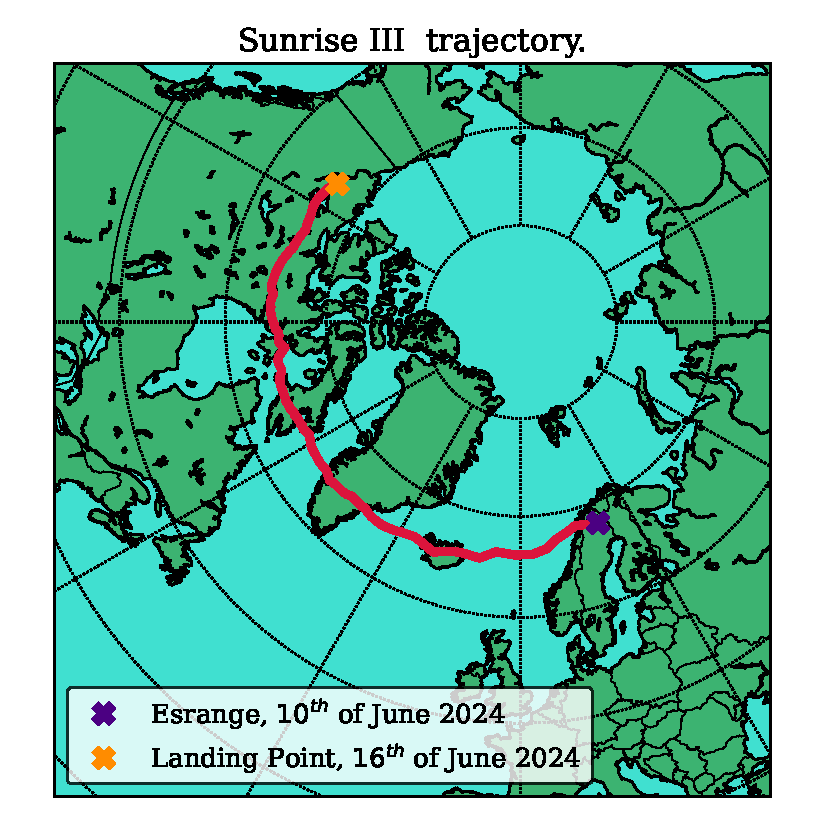
\includegraphics[width = \textwidth]{figures/Introduction/SunriseIII_trajectory.pdf}
  \caption{Sunrise III trajectory.} 
  \label{fig_intro: sunrise_trajectory}
\end{figure}


It wasn't until the $10th$ of July of 2024 that Sunrise III got its second chance to fly, and this time, the opportunity was not wasted. After a very succesful flight that lasted 6 days, the observatory landed in the northern region of Canadá on the XX of July. Figure XX shows the trajectory our favourite solar observcatory followed over this days. The recovery process started immediately after landing, and we were able to lay hands on the data for the first time on September 2024. 

In the following chapters, we will present the work undertaken during the calibration and commissioning of TuMag, conducted in 2021, 2022, and 2024. Additionally, the research carried out between the first and second flights of Sunrise III, which has resulted in the publication of two articles as the main author — one published in APJ and the other in A\&A — will also be detailed in this manuscript, as well as other studies that have not yet been published in any scientific journal. 


\section{Motivation of our work}

In experimental sciences, there is a very strong relation between technological and scientific advances due to the simple fact that we cannot draw conclussions from what we cannot see. We believe it is important for experimental scientists, and more specifically, for observational astronomers, to know the limitations and capabilities and understand the functioning of the instruments we use. 

This philosophy is one of the pillars of this thesis, which covers topics ranging from the design and calibration of scientific instruments to the exploitation of the data they produce. With this thesis, we aim to provide a broad, yet detailed, view of the various stages of a scientific mission, from its conception and objectives through its design and calibration, data reduction and preparation for scientific exploitation, and finally, the studies and conclusions derived from it.

In particular, we will detail this process within the framework of solar physics through the development of TuMag, the magnetograph aboard Sunrise III. We will present the scientific objectives of the mission and attempt to link the design concepts with the scientific questions we aim to answerr. We will address the challenges encountered in data correction due to the technical or instrumental limitations, a subject of ongoing debate within the community and of current relevance. And finally, we also aim to offer a brief dip into the scientific explotation that can be carried out with the final data product. 

With this thesis we aim to clarify the following points:

\begin{itemize}
  \Myitem Scientific objectives of TuMag.
  \Myitem Instrumental ways of achieving the scientific purposes
  \Myitem Open problems for data reduction. Flat-fields, etalon effects in the data. 
  \Myitem Offering an example of data exploitation with aa study case. Persistent Homology.
\end{itemize}

\section{Introduction}

Astronomy is one of the broadest fields of knowledge. It studies everything from the smallest astronomical objects, such as the small asteroids that inhabit our solar system, to the global structure and evolution of the universe, including the study of planetary systems, stars, black holes and the galaxies in which they are found. However, despite the diversity of disciplines—ranging from stellar astronomy, radio astronomy, and cosmology, to extragalactic astronomy, astrobiology, and solar physics—they all share a common tool for studying the cosmos: light. Since the very beginning of astronomy, the astronomer's work has been to learn how to modify and measure the properties of the photons that reach us in order to infer the characteristics of the observed object. Although recent advancements have provided astronomers with new lenses to \textit{see} the cosmos, like gravitational waves (\textbf{REFERENCIA}) or neutrinos (\textbf{REFERENCIA}), among others, light remains as our main resource. Our understanding of the cosmos has always gone hand-in-hand with our ability to design and develop new (or more efficient) and clever ways to disect the light, spanning from the first solar clocks, passing through Newton's first telescope to the modern-day spaceborne telescopes like the Hubble, James Webb or Solar Orbiter. 

Solar physics is no different from other astronomical disciplines in this regard. Our main tool to \textit{see} the Sun is through light. Contrary to what one may think, solar physicists are as photon-starved as any other astronomer. Even though our star is closer and (apparently) brighter than any other astronomical object, our requirements regarding resolution and sensitivity are so high that we are as dependent on extremely optimized instrumentation as any other discipline. Thus, the development of instrumentation employing state-of-the-art technology and techniques plays an important role in modern solar physics.


\section{A brief introduction to spectropolarimeters.}

Spectropolarimeters, as suggested by the name, are devices that measure the spectral and polarimetric properties of light, or in other words, that measure the polarization state of light as a function of wavelength. Their use is widely extended in astrophysics due to the huge amout of information about the light source we can infer from these properties.

In solar physics, it is common to encounter two distinct types of spectropolarimeters, distinguished by their approach to spectroscopy: slit-based spectrographs, such as SUSI and SCIP, and narrow-band tunable filtergraphs, like TuMag. The latter preserve spatial resolution by capturing two-dimensional images of the solar scene at the expense of sacrificing spectral resolution. Conversely, slit-based spectrographs provide excellent spectral resolution but have a limited spatial resolution. 

Regardless of how spectroscopy is carried out, spectropolarimeters must be able to measure the polarization state of light. That is, they must be capable of determining the Stokes parameters  of the incident light. These four parameters, usually grouped in a pseudo-vector: $[I, Q, U, V]$, were defined by Stokes in \cite{Stokes_vector} as a mathematical formalism to completely define to polarization state of light. The first parameter, $I$, represents the total intensity; $Q$ and $U$ provide information about the intensity of linearly-polarized light, at 0º and 90º, respectively; and lastly, $V$, accounts for the intensity of circularly polarized light. 

Excellent polarimetric sensitivity and spectral resolution are wasted if the optical capabilities of the instrument are not up to par. The design of these instruments must achieve diffraction-limited imaging, with a signal-to-noise ratio ensuring a polarimetric sensitivity of 1000 (typically), and the best spatial resolution the telescope allows, all without sacrificing spectral resolution and accomplishing this in the shortest possible time.

When designing the instrument, one must balance these three properties: spectral, optical, and polarimetric capabilities, trying to improve the performance in all of them without sacrificing too much. In the following sections, we will delve into each of these aspects in more detail.

\subsection{Imaging.}

Filtergraphs are, first and foremost, imagers. The high-resolution imaging that filtergraph instruments are capable of is one of the pivotal reasons for their extended use. The ability to capture a two-dimensional scene of the solar surface makes them ideal for studying solar plasma structures, which require resolutions close to 100 km on the solar photosphere. These instruments must be able to ensure an image quality and resolving power enough to measure these structures. For this reason, we will begin our description of the filtergraphs with a brief explanaiton of image formation and image quality assessment. 

Let us assume that the extended source we are observing has a instensity distribution in the image plane given by $O(\xi _ 0, \eta _ 0)$. Then, if we assume a linear optical system and incoherent illumination, the intensity distribution measured at a point $\xi, \eta$ of the image is given by : 

\begin{equation}
  I_ j\left(\xi, \eta ; \lambda_{s}\right)= \iint  O\left(\xi_0, \eta_0\right)  \mathcal{S}\left(\xi_0, \eta_0; \xi , \eta;\right)  \mathrm{d} \xi_{0} \mathrm{~d} \eta_{0},
  \label{eq_spectro: intensity_simple}
\end{equation}
where $\mathcal{S}\left(\xi_0, \eta_0; \xi , \eta;\right)$ represents the imaging response of the instrument, also referred to as the Point Spread Function (PSF). The PSF describes the normalized intensity distribution in the image plane when observing a point source, which, due to diffraction and inherent imperfections in any imaging system, cannot be imaged as an ideal point.

The PSF is crucial in the assessment of image quality and resolving power of an instrument since it defines how fine detail will be imaged into the detector. One particularly relevant metric for image quality assessment that can be derived from the PSF is the modulation transfer function (MTF). The MTF, in turn, is obtained from the optical transfer function (OTF), which is the Fourier transform of the PSF \citep{vargas_tesis}. 

\begin{equation}
  OTF(\nu) = \mathcal{F}\left[\mathcal{S}\left(\xi_0, \eta_0; \xi , \eta;\right)\right],
\end{equation}
where the operator $\mathcal{F}$ is the Fourier transform, and $\nu$ the spatial frequencies.

The OTF describes how different spatial frequencies are transferred from the object to the image, thus characterizing the system's ability to resolve fine details. However, since imaging systems measure intensities, we are primarily concerned with how the intensity pattern of an object is transferred to the image. A key metric for quantifying this transfer is modulation, or contrast, which is defined as the ratio between the peaks and valleys of intensity at a given spatial frequency:

\begin{equation}
  M _ {\nu} = \frac{I_{max} ^{\nu} - I_{min} ^{\nu}}{I_{max} ^{\nu} + I_{min} ^{\nu}},
\end{equation}

which is strictly related to the OTF as the ratio of the modulation of the object $MTF_{obj}$ and that of the image $MTF_{im} $can be computed from the magnude of the OTF \citep{OTF}:

\begin{equation}
  \frac{MTF_{im}(\nu)}{MTF_{obj}(\nu)} = | OTF(\nu) |.
\end{equation}

From this definition, it is evident that a perfect optical system would have an $MTF=1$ at all spatial frequencies, meaning that all details are perfectly transferred from the object to the image. However, real optical systems exhibit a decrease in MTF as spatial frequency increases. In practice, the resolution of an optical system can, and is often defined as the spatial frequency at which both the MTF and, consequently, the OTF reach zero \citep{wfes}. This threshold frequency marks the limit beyond which the system can no longer resolve finer details. 

Another key concept for assessing the imaging performance is the phase error or wavefront. The wavefront of an optical system is defined as the deviation in phase at any point within the image from that of an ideal spherical wavefront \citep{WFE_def}. Such deviations arise from various optical imperfections within the imaging system, and their impact on image quality depends on the specific nature of the aberration. For instance, imperfections in mirror shape or lens configuration can result in spherical aberrations, leading to a broadening of the point spread function (PSF) and a subsequent reduction in resolution. Other common aberrations include astigmatism, where the focal point varies along different axes, producing distorted images, and comatic aberrations (coma), which can occur due to misalignment of optical elements and manifest as tail-like distortions in the images of point sources.

It is common to see requirements or assessment of the optical quality in terms of the root mean square (rms) of the variance of the wavefront, $\Delta \phi (\xi, \eta)$, usually refered to as wavefront error (rms WFE) or simply WFE:

\begin{equation}
  WFE = \sqrt{\frac{1}{A}\int _ {A} \left( \Delta \phi (\xi, \eta) \right) ^2 \mathrm{d \xi}\mathrm{d \eta}},
\end{equation}
where $A$ is the area of the aperture. 

This value, essentially the standard deviation of the wavefront across the FoV, is closely tied to beam propagation quality. In fact, it can be demonstrated that the wavefront variance can be derived from the Strehl ratio, or conversely, the Strehl ratio can be computed from the wavefront error. The Strehl ratio is defined as the ratio of the peak intensity of a point source in an aberrated system to that of an ideal system operating at the diffraction limit. It is one of the most widely used metrics for assessing the optical quality of a system, ranging from 1, for a perfect, unaberrated system, to 0. For small aberrations, the Strehl ratio (SR) and WFE are related by the following expression \citep{WFE_def}: 

\begin{equation}
  SR \simeq \exp \left[ - \left(\frac{2\pi WFE}{\lambda}\right) ^2 \right].
\end{equation}

Although the Strehel ratio and rms WFE provide a concise measure of the optical quality of a system, the WFE contains additional information that can further elucidate imaging performance. Rather than relying solely on a single averaged value (such as the standard deviation), the wavefront can be represented as a two-dimensional map projected onto a plane normal to the light path, typically the image plane. To carry out such a representation analytically, it is essential to select an appropriate mathematical framework. Given the widespread use of circular apertures in telescopes, mirrors, lenses, and other optical components, it is advantageous to approach the problem using polar coordinates, and in particular, to employ an orthonormal basis for theinterpretability of the results. Among the multiple (infinite) sets of polynomials that fullfill these requirements, the Zernike polynimals \citep{Zernike} offer some distinct advantages. The Zernike polynomials are a sequence of polynomials that compose an orthonormal basis over a unit circle. Given an arbitrary wavefront, ($W(\rho, \theta)$), the expansion in terms of the Zernike polynomials can be expressed as \citep{Zernike_guide}:
\begin{equation}
  W(\rho, \theta) = \sum_{n, m} C _n ^m Z _ n ^m(\rho, \theta),
\end{equation}
where $Z _n ^m$ are the Zernike polinomyals, $C_n ^m$ are the amplitues of the coeffiecients in the expansion and $n$ and $m$ are the radial order and angular frequency, repectively. 

This represntation of the wavefront is of special interest since each mode (a particular value for $n$ and $m$) corrsponds to a specific aberration of the wavefront, and the value of the coefficient represents the rms WFE associated to that specific aberration. Additionally, the orthogonality of the basis ensures that the addition of terms into the expansion does not affect the value of the previous. Therefore, the Zernike polynomial expansion allow us to describe the wavefront as the sum of all the individual aberrations. 

\begin{figure}
  \centering
  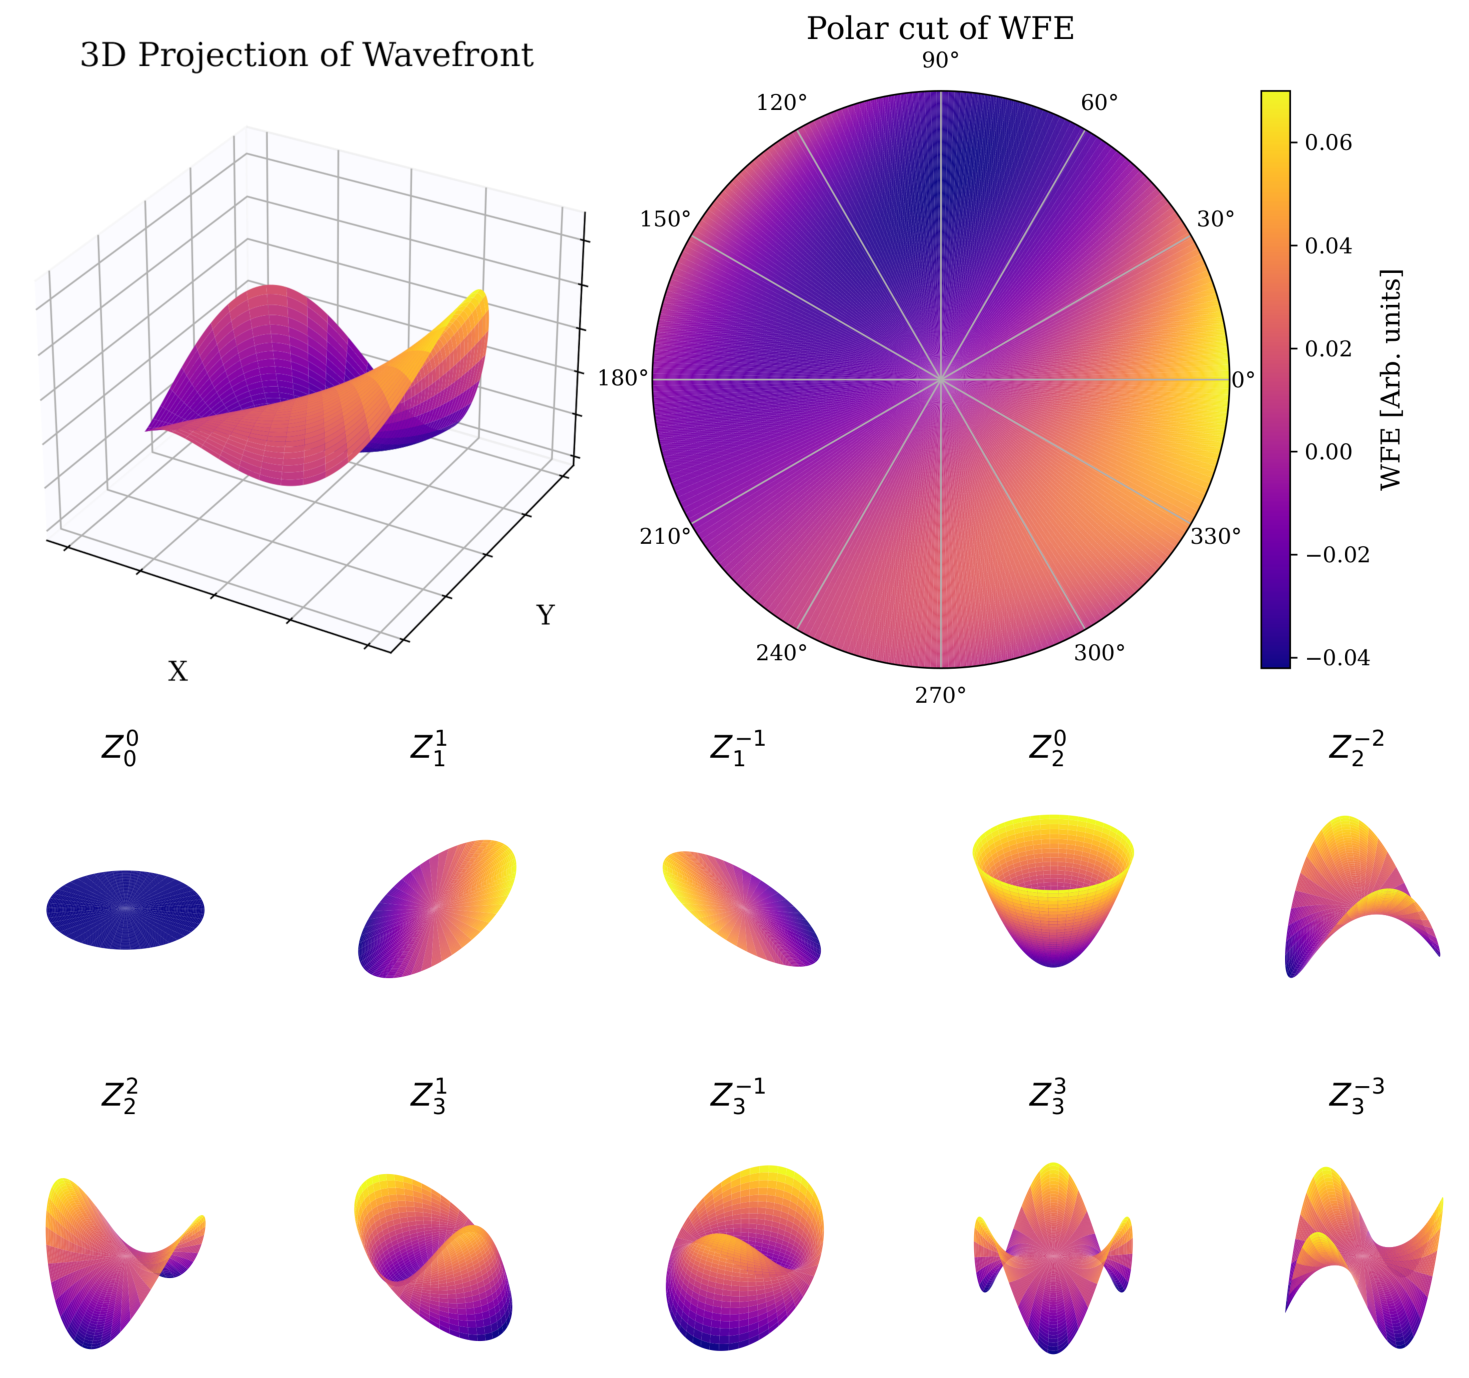
\includegraphics[width = \textwidth]{figures/Introduction/zernikes_combined.pdf}
  \caption{Sunrise III trajectory.} 
  \label{fig_intro: sunrise_trajectory}
\end{figure}

\subsection{Spectroscopy}

Narrow-band tunable spectrographs play a significant role in this thesis. They will be extensively discussed in this chapter, particularly in relation to the design and calibration of TuMag, and again in Chapters \ref{CH:Pipeline} and \ref{CH:challenges} when addressing TuMag's pipeline and the correction of data produced by these instruments. Therefore, for the sake of simplicity, we will focus exclusively on this type of spectrographs from this point onward.

\textcolor{red}{CAMBIAR ESTO}.

Fabry-Pérot Interferometers (FPIs), also known as etalons (used interchangeably), represent one of the most prevalent forms of narrow-band tunable spectrographs. Composed by a resonant optical cavity formed by two distinct optical media, these devices allow only the passage of light with wavelengths corresponding to constructive interference within the cavity. 

The transmission profile of an etalon, being produced by an interference phenomenon, is characterized by a series of narrow and periodic transmission peaks. The wavelengths at which this resonance peaks are located, their width, and their separation are determined solely by the physical properties of the etalon. In fact, it is not difficult to demonstrate \citep{franI} that a resonant cavity produces a periodic transmission profile, with maxima occurring at a wavelength $\lambda$ such that:

\textcolor{red}{REVISAR -> VÁLIDO PARA TELECENTRIC??} 

\begin{equation}
\lambda = \frac{2nd\cos \theta}{m}\ ,
\label{eq_ch2: order_sorting}
\end{equation}
where $n$ is the refractive index of the medium inside the cavity, $d$ is the distance between the mirrors, $\theta$ is the angle of incidence of the incoming light ray and m is the interferential order ($m \in \mathbb{Z} $). 

With Eq.~\eqref{eq_ch2: order_sorting} in mind, it is clear that an etalon allows for tuning the wavelengths of the transmission peaks by either changing the distance between the mirrors or by altering the refractive index. Although changing the angle of incidence also results in a wavelength shift, it introduces other issues, such as ghost images or profile broadening in telecentric configurations, among other effects. Consequently, the angle is not used for wavelength tuning.

To tune to a single wavelength (or a very narrow band around it), it is necessary to isolate one transmission peak (main order). This is typically achieved by using a pre-filter that only allows light with wavelengths near the desired measurement region to pass through. This ensures that no light reaches the etalon that could pass through it due to interference orders other than the main one (secondary orders). 

\begin{figure}
  \centering
  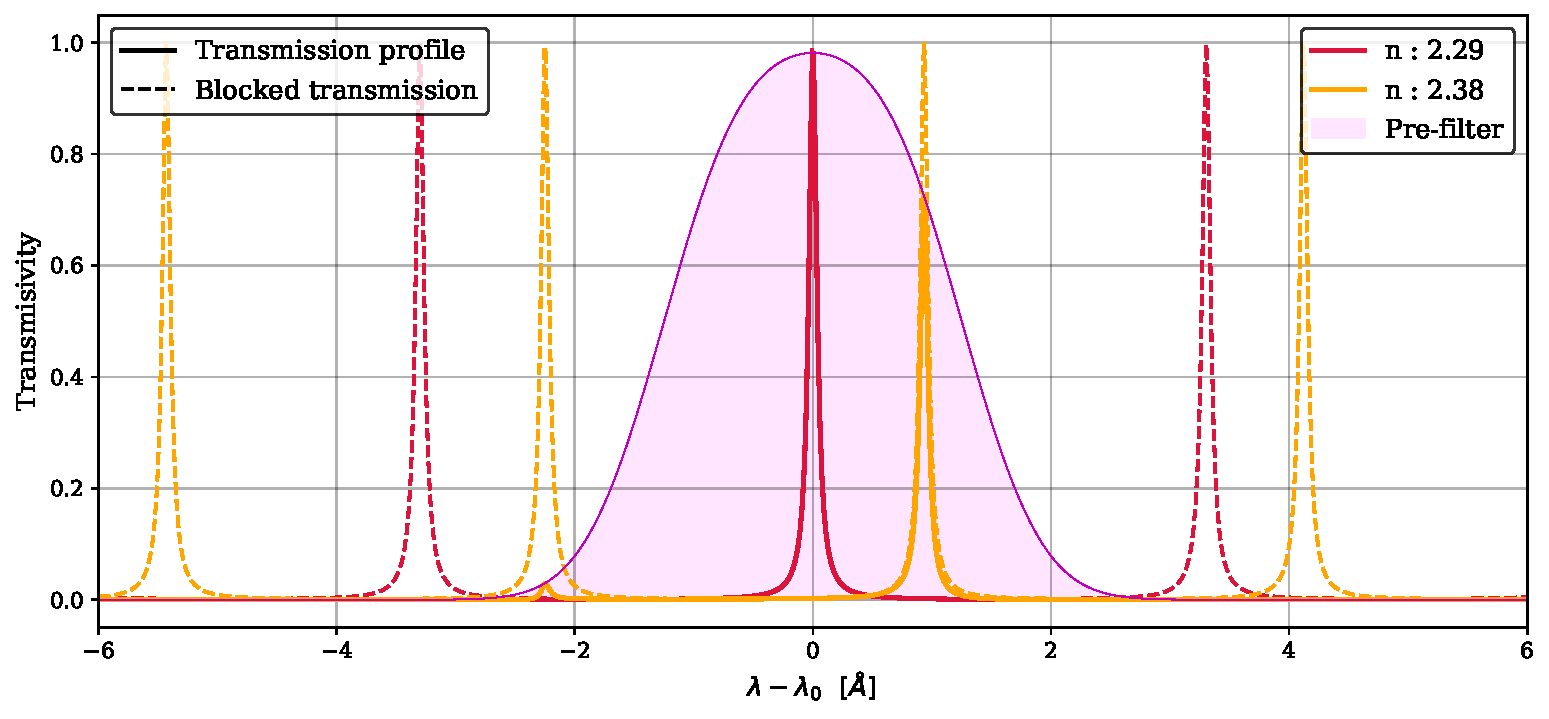
\includegraphics[width = \textwidth]{figures/Introduction_to_spectropolarimeters/Etalon_and_prefilter_example.pdf}
  \caption{Transmission profiles of the same etalon with varying refractive indices (n). The dashed lines represent the original transmission profile, while the solid lines indicate the portion of the transmission profile that passes through the order-sorting pre-filter (shaded purple area).} 
  \label{fig_ch2: etalon_example}
\end{figure}

Figure \ref{fig_ch2: etalon_example} shows a simulation of the spectral behavior of this optical setup. The order-sorting pre-filter is shown with a shaded purple area and the unaltered transmission profile of the etalon is shown in dahsed lines for different values of the refractive index. In solid lines, the resulting transmission profile is shown, that is, the transmission allowed through both the pre-filter and etalon at the same time. 

\subsection{Polarimetry}

\textcolor{red}{As previously noted, determining the polarization state of light requires the determination of the components of the Stokes vector. However, these parameters cannot be measured directly since we only know how to measure intensities. Since they are  Thus, measuring the polarization of light always involves multiple measurements at once. Specifically, a number equal to the number of elements to be determineed: four for the complete Stokes vector, or two, if only the circular polarization and total intensity are to be measured. This is the root of the difficulties in measuring polarization, as the need for multiple measurements makes them much more susceptible to spurious effects compared to individual measurements.} Cambiar que es un jaleo. 

Mathematically, the effect on polarization of a linear and finite system can be treated as a combination of linear transformations on the Stokes vector and, therefore, can be represented by a matrix in $\mathbb{R}^4$, known as the \textit{Mueller Matrix}. Let $\textbf{M}$ be the matrix that describes these transformations, then the polarization state that reaches the detector follows:

\begin{equation}
  \textbf{I}_{out} = \textbf{M}\textbf{I}_{in},
\end{equation}
where $\textbf{I}_{in}$ and $\textbf{I}_{out}$ are the Stokes vectors of the light that reaches the instrument, and the detector, respectively. However, since we only know how to measure intensities, the actual quantity measured by our CCD is: 

\begin{equation}
  I_{obs} = m_{00}I_{in} + m_{01}Q_{in} + m_{02}U_{in} + m_{03}V_{in} \ \ ,
\end{equation}
where $m_{0i}$ is the i-th element of the first row of the Mueller Matrix. This means that the intensity we measure is a linear combination of the different polarization states of the incoming light. To determine the values of the individual parameters $I_{in}$, $Q_{in}$, $U_{in}$, and $V_{in}$, further independent measurements are necessary, which can be achieved by modifying the Mueller matrix. In particular, it is easy to see that four independent measurements are required in order to construct a system of equations that allows us to determine the full Stokes vector. This process is known as modulation, and the four independent measurements are referred to as modulations.

If we denote each of the modulations by $I _ j$ with $j \in \left\{ 1, 2, 3, 4\right\}$, we can construct the following system of equations:

\begin{equation}
  \begin{pmatrix}
  I _ 1 \\
  I _ 2 \\
  I _ 3 \\
  I _ 4
  \end{pmatrix} = 
  \underbrace{\begin{pmatrix} 
      m ^ 1 _ {01} & m ^ 1 _ {02} & m ^ 1 _ {03} & m ^ 1 _ {04} \\ 
      m ^ 2 _ {01} & m ^ 2 _ {02} & m ^ 2 _ {03} & m ^ 2 _ {04} \\
      m ^ 3 _ {01} & m ^ 3 _ {02} & m ^ 3 _ {03} & m ^ 3 _ {04} \\
      m ^ 4 _ {01} & m ^ 4 _ {02} & m ^ 4 _ {03} & m ^ 4 _ {04} 
  \end{pmatrix}}_ {\textbf{O}}
  \begin{pmatrix}
    I _ {in} \\
    U _ {in} \\
    Q _ {in} \\
    V _ {in}
    \end{pmatrix} \, 
    \label{eq_spectro_theory: stokes_linear_comb}
\end{equation}
where the superindex in $m ^j _{oi}$ denotes the values of the Mueller Matrix for each modulation. Through straightforward algebra, it is easy to see that the stokes vector of the incoming light can be determined by $\textbf{I}_{in} = \textbf{D}\textbf{I}_{obs}$, where $\textbf{D}$ is the demodulation matrix, the inverse of the modulation matrix, $\textbf{O}$, and $\textbf{I}_{obs}$ is the vector containing the 4 measured modulations. Accurately determining $\textbf{O}$ during the instrument calibration process is crucial, as the determination of the Stokes components depends entirely upon it.

\subsection{\label{susec_spectropolarimeters: Imaging}Imaging}

\textcolor{red}{The high-resolution imaging that etalon-based instruments are capable of is one of the pivotal reasons for their extended use. The ability to capture a two-dimensional scene of the solar surface makes them ideal for studying solar plasma structures, which require resolutions close to 100 km on the solar surface. However, it is essential to achieve these resolutions while maintaining a sufficiently high signal-to-noise ratio to ensure the required polarimetric sensitivity.}

Spectropolarimeters ultimately combine measurements in polarization, spectral, and spatial (image) domains. Consequently, the final observed intensity depends on all three properties simultaneously. By integrating the spectral behavior of the etalon and pre-filter with the polatrimetric measurements, and taking into account the spatial dependence of these measurements, the observed intensity for a modulation $j$ at any point of the focal plane $\eta, \xi$ when the etalon is tuned at a wavelength $\lambda _ s$ is determined by:

\begin{equation}
  I_ j\left(\xi, \eta ; \lambda_{s}\right)=g(\xi, \eta)\int_{0}^{\infty} T(\lambda) \iint  O _ j\left(\xi_0, \eta_0 ; \lambda\right)  \mathcal{S}\left(\xi_0, \eta_0; \xi , \eta; \lambda-\lambda_{s}\right)  \mathrm{d} \xi_{0} \mathrm{~d} \eta_{0}\mathrm{d} \lambda ,
  \label{eq_spectro: General_Intensity}
\end{equation}
where $T(\lambda)$ accounts for the presence of the order-sorting pre-filter, $S\left(\xi_0, \eta_0; \xi , \eta; \lambda-\lambda_{s}\right)$ accounts for the imaging response of the instrument when tuned at the wavelength $\lambda_{s}$, $g(\xi, \eta)$ represents a spatial gain factor that accounts for any wavelength independent pixel-to-pixel intensity fluctuations ocurring in the focal plane, and $O _ j(\xi_0, \eta_ 0;\lambda)$ is the intensity distribution of the incoming light for a modulation j and is given by:
\begin{equation}
  O _ j(\xi_0, \eta_ 0;\lambda) = m_{00} ^jI_{in}(\xi_0, \eta_ 0;\lambda) + m_{01}^jQ_{in}(\xi_0, \eta_ 0;\lambda) + m_{02}^jU_{in}(\xi_0, \eta_ 0;\lambda) + m_{03}^jV_{in}(\xi_0, \eta_ 0;\lambda)
\end{equation}

Determining the imaging response of the instrument can be quite complex , as it is influenced not only by their physical characteristics but also by their optical configuration, whether collimated or telecentric. In Chapter 2, we provide a detailed overview of the properties of each configuration, their differences, and the challenges involved in using these devices for data correction.

Strehl ratio and Wfront error. 
Wilson, R. N. (2004). Reflecting Telescope Optics I: Basic Design Theory and its Historical Development. Springer.
Schroeder, D. J. (2000). Astronomical Optics. Academic Press.
Beckers, J. M. (1993). "Adaptive Optics for Astronomy: Principles, Performance, and Applications". Annual Review of Astronomy and Astrophysics, 31, 13-62.

SPEAK ABOUT PD. 

\textcolor{red}{ADD noise Discussion?}
 
\subsection{What do spectrpolarimeters tell us about the Sun?}

Spectropolarimeters are often referred to as magnetographs (\textit{e.g.}, TuMag), suggesting they measure magnetic fields directly. However, this is not entirely accurate. In astrophysics, the physical properties of the light source are inferred by correlating them with the observed properties of the light, rather than measuring them directly. By evaluating the polarization of sunlight at different wavelengths, spectropolarimeters enable us to infer the magnetic field and estimate plasma velocities on the solar surface. 

The simplest calculation we can carry out that provides us with physical quantities of the Sun is that of the line-of-sight (LOS) velocities. Given the spectral shift of a specific absorption or emission spectral line, $\Delta \lambda$, with respect to its rest position, $\lambda _ 0$ , the LOS velocities can be computed with the Doppler formula: 
\begin{equation}
  v_{LOS} = \frac{\Delta \lambda}{\lambda _ 0}c\ \ ,
  \label{eq_spectro: Doppler}
\end{equation}
where $c$ stands for the speed of light in vacuum. 

The polarization properties of light come into play when determining the magnetic fields. Due to Zeeman and Hanle effects, the polarity and spetcroscopy of spectral lines can be altered when formed in the presence of magnetic fields. Due to the Zeeman effect, the spectral lines widen or split into different polarized components when a strong magnetic field is present \citep{libro_JoseCarlos}, such as in the surroundings of sunspots and active regions. In the other hand, the Hanle effect is sensitive to weaker fields, and can be used to study the magnetic structure of solar prominences or turbulent fields in the solar photosphere \citep{hanle}. 

One simple strategy to employ polarization and spectral data to derive the magnetic fields is through the center-of-gravity method. According to \cite{center_of_gravity}, the LOS strength of the magnetic field can be obtained through:
\begin{equation}
  B_{LOS} = \frac{\lambda _ {+} - \lambda _ -}{2}\frac{4\pi m c}{eg_{L}\lambda_0 ^2}\ \ ,
  \label{eq_spectro: Blos-cog}
\end{equation}  
where $m$ and $e$ are the electron mass and charge respectively, $g_L$ stands for the Landé factor and $\lambda _ {+}$ and $\lambda _ {-}$ are the centroids of the right and left circularly polarized line components, respectively, and are computed by:
\begin{equation}
  \lambda _ {\pm} = \frac{\int \lambda \left[I_{cont} - (I \pm V)\right]d\lambda}{\int \left[I_{cont} - (I \pm V)\right]d\lambda} \ ,
  \label{eq_spectro: lambda_plus_minus}
\end{equation} 

where the subindex "$cont$" stands for the wavelength at the continuum. 

The vector magnetic field (\textit{i.e.}, strength, azimuth and inclination), and not only the LOS strength can also be derived. However, the derivation of these quantities has to be achieved through inversions of the radiative transfer equation (RTE). The applicability of the different methods to carry out this inversion is an extensive topic as there are some assumptions that can be applied in some cases but not in others, such as the weak-field or Milne-Eddington approximations, among others. For an extended discussion of this topic, we refer the interested reader to \cite{del2016inversion}.   

% Spectropolarimters and Tumag
%\chapter{Sunrise III and TuMag: Design and calibration.}

The first chapter ...


\section{Sunrise III}

Equipped with a telescope with a 1m aperture, two slit-based spectropolarimeters and an imaging magnetograph, the Sunrise III observatory is the most complex solar telescope to ever leave the the ground. The coordination of three different scientific insturments allows Sunrise to simultaneously perform narrow-band polarimetric imaging in the visible while carrying out spectropolarimetry in the near-UV and near-IR, from the advantageous point of observation of $\sim$ 36 km of altitude whithout the anoying interference of the atmosphere's turbulence. 

The three instruments aboard Sunrise III have been carefully designed to complement each other and address the scientific purposes of the mission. The Tunable Magnetograph (TuMag, REF), developed by the Spanish Solar Space Consortium (S³PC), carries out high-spatial-resolution imaging spectropolarimetry in the visible range of light. Able to tune to three different spectral lines, namely the highly Zeeman-sensitive iron lines at 525.02 and 525.06 nm, and the Mg I b$_2$ line, TuMag can probe the photosphere and low chromosphere quasi-simultanously. 

The absence of atmosphere allows the Sunrise Spectropolarimeter and Imager (SUSI, Ref), developed by the Max planck), to observe in the near-UV, performing imaging and spectropolarimetry in the range of 309-417 nm. The high polarimetric sensitivity and large number of spectral lines present in this range, many of which are sensible to the Hanle effect, allows SUSI to sample many heights in the solar atmosphere at the same time while measuring the weak magnetic fields. 

In the same way that the atmosphere complictaes the observations of the UV range from the ground, observations of many lines in the near-IR are also unfeasable with ground-based instruments due to the telluric contamination of the atmosphere. The Sunrise Chromospheric Infrared spectro-Polarimeter (SCIP, REF), developed by ...,  takes advantage of the abscence of atmosphere and observes two of the Ca II triplets lines. Spectropolarimetry measurments of these lines provides information of the 3-D structure of the chromosphere and its magnetic fields, derived thanks to the high zeeman sensitivity of the selected lines. Furthermore, the large number of available photons at these wavelengths ensures a high (S/N) and polarimetric sensitivities. 

The ability to probe simultanously the near-IR, the visible and the near-UV, perfoming high-resolution polarimetric imaging and spectroscopy makes Sunrise III an unique observatory, capable of studying the the connection  and interaction of the small-scale phenomena ocurring at different layers of the solar's atmosphere with unprecedented detail and completeness. 

\begin{figure}
    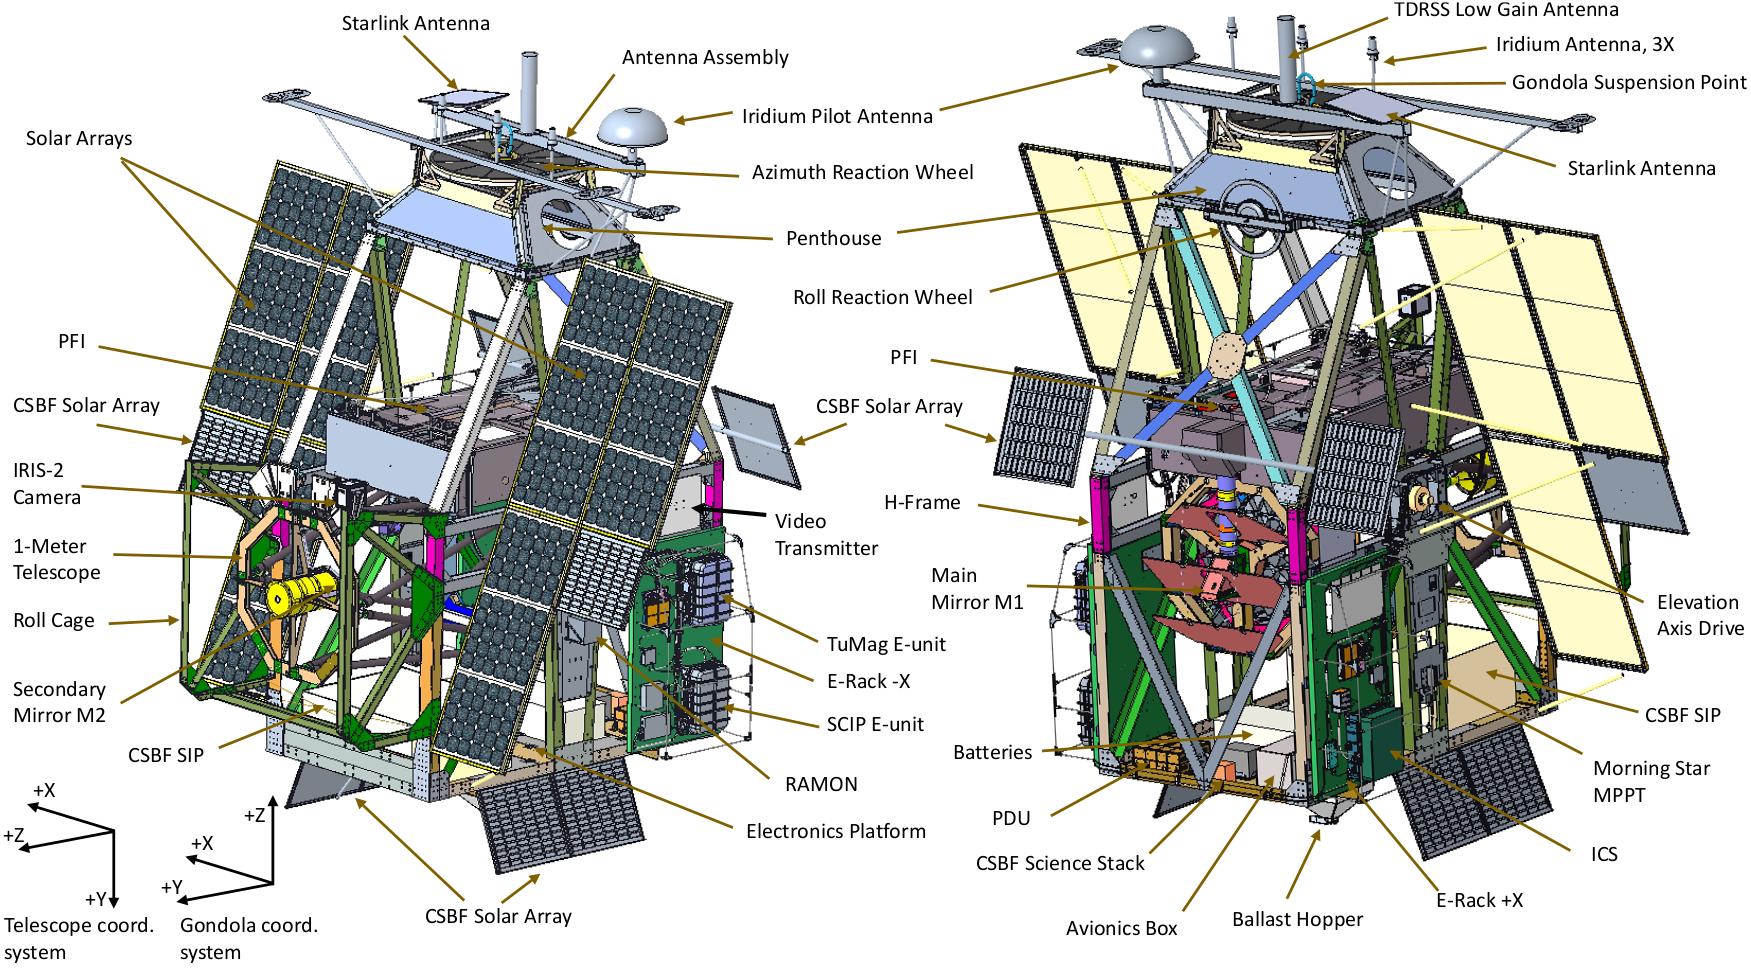
\includegraphics[width=\textwidth]{figures/TuMag/Sunrise_schematic.png}
    \caption{
      Drawing design of the Sunrise III observatory. Image reproduced from XXXXX with permission. \textcolor{red}{No he pedido permiso para esta aún, que es del paper de Sunrise III que mandó Andi, pero creo que quedaría bien algo enseñando el observatorio. Al no estar pulicado el paper de Sunrise no se muy bien cual coger.}}
      \label{fig: SunriseIII}
\end{figure}

\subsection{Observatory's design}

Sunrise III is the result of many years of work carried out by many people belonging to various international institutions.  While the scientific instruments are central to the research facilitated by Sunrise, several additional subsystems play a crucial role, each contributing to the overall success of the mission.

The structural framework housing all components of the observatory, as well as the interface connecting the observatory to the flight apparatus, is provided by the gondola. This gondola was engineered by the Johns Hopkins University Applied Physics Laboratory (APL, USA). Beyond safeguarding the instruments and telescope during ascent and landing, the gondola is tasked with ensuring the stability of the pointing system. Given that the observatory is suspended from a balloon, it is subject to wind-induced motion and pendulum-like oscillations, which threaten the stability required for prolonged observations. The gondola’s pointing control system (PCS) must actively counteract these disturbances in real time by making precise adjustments to the telescope’s elevation and azimuth. In conjunction with the Correlating Wavefront Sensor (CWS), developed by the Institut für Sonnenphysik (KIS, Germany), which is responsible for image stabilization and autofocus, the PCS was required to achieve a pointing accuracy better than 0.005" root mean square (rms) over extended periods to facilitate long-duration observations.

The Sunrise III telescope is a Gregory-type reflector with a 1-meter aperture, featuring a 234 mm central obscuration and an effective focal length of 24.2 meters. This configuration provides a field of view (FoV) of 3.4', corresponding to approximately 150 Mm on the solar surface. The telescope directs light to the post-focus instrumentation platform (PFI), located above the telescope. The PFI houses the three scientific instruments and the CWS, and is responsible for distributing light among these four instruments. This distribution, performed by the Image Stabilization and Light Distribution Unit (ISLiD), must efficiently separate the different wavelengths in a photon-efficient manner to provide the highest number of available photons to each instrument. 

While all the subsystems discussed thus far directly influence the optical performance, it is equally important to recognize the crucial role played by other subsystems, such as the electronics and software control. In particular, the Instrument Control System (ICS) is responsible for the management of the observatory, gathering housekeeping and issuing commands to the electronic units of each instrument. As will be elaborated in the following chapter, Sunrise III observations were designed to operate in a semi-autonomous manner through the use of pre-programmed timelines. This approach requires that all electronic systems function in synchrony, with minimal human intervention. 

\subsection{Science with Sunrise.}

As previously mentioned, the absence of Earth's atmosphere opens the window for IR and UV observations and offers a level of image stability that cannot be achieved in ground-based observatories due to atmospheric seeing. However, these advantages are also present in spaceborne missions, such as the Spectro-Polarimeter and Narrowband Filter Imager aboard the Solar Optical Telescope (SP/NFI-SOT) of the Hinode mission (\citealt{Hinode}, \citealt{sot}), or the Polarimetric and Helioseismic Imager aboard Solar Orbiter (SO-PHI) (\citealt{PHI}, \citealt{SO}), among others. Nonetheless, spaceborne missions have strong restrictions regarding payload, mass and data rate. 

The abscence of these restrictions in balloon-borne observatories allows for a more complex and versatile instrumentation than the one present in space missions. The combinnation of these two factors, namely the absence of atmosphere and the complex and advanced instrumentation they can carry, places observatories such as Sunrise in an unique position, and provides them with unique presepectives on solar phenomena.

Many aspects of the physical processes driving our Sun remain unresolved. The mechanisms underlying various solar phenomena are still the subject of debate, ranging from the origin and removal of magnetic flux in the solar photosphere to the processes responsible for heating the chromosphere and corona, as well as the small-scale dynamics of solar plasma. The three instruments aboard Sunrise work in consoncance to provide novel insights into these phenomena, potentially helping to unravel the mysteries surrounding them.

The magnetic field, present across multiple scales and heights, is the principal driver of solar activity. Understanding the magnetic field is essential for comprehending the processes that govern solar phenomena, energy distribution, and plasma dynamics. Thus, numerous works direct their efforts to the study of the structures and evolution of magnetic fields. For instance, several works study  the emergence of magnetic flux in the photosphere, such as, \cite{flux_emergence_1} and \cite{flux_emergence_2}, where they utilized Sunrise I IMaX data to examine small-scale flux emergence events occurring within solar granules. Likewise, the processes responsible for magnetic flux removal are not fully known. Several studies, such as \cite{flux_removal_1} and \cite{flux_emergence_2}, have proposed mechanisms for flux removal in the photosphere; however, no model is favoured over the other by current observations.

A thorough 3-dimensional analysis of the magnetic fields is essential to study these events. The combination of spectropolarimeters and vector magnetographs aboard Sunrise, which are capable of measuring strong magnetic fields through the Zeeman effect, and detecting weaker, more turbulent \citep{quiet_sun_living_review} magnetic fieldsusing the Hanle effect - particularly sensible in the UV - can provide a new and complete perspective of these events.  

Chromosphere


Helioseismology. 


\section{The Tunable magnetograph: TuMag}

The Tunable Magnetograph (TuMag) is a tunable imaging spectropolarimeter designed to deliver high spatial resolution images across multiple spectral lines in four distinct polarization states. Consequently, TuMag is capable of measuring the four Stokes parameters, thus enabling the inference of the three components of the magnetic field and the LOS velocities at all the selected spectral lines. Moreover, this data must be acquired following a series of strict requiremets regarding optical quality, polarimetric efficiencies, required SNR, spectral performance and time limitations. A summary of these requirements is provided in Table \ref{table: Tumags requirements}. 

\begin{table}
    \centering
   \begin{tabular}{cc}
    \hline
    \hline
    Requirements & Value \\
    \hline
    Field of view & $63''$ x $63''$ \\
    RMS wavefront error & $W \sim \lambda / 14$\\
    Spatial sampling & $3 \times 3 $ pixels \\
    Plate scale & $0.0378''$ / pixel \\
    Polarimetric efficiencies & $\epsilon _ {1, 2, 3} \lessapprox \frac{1}{\sqrt{3}}$\\
    SNR ratio & $\left(\frac{S}{N}\right) _ 0 \gtrapprox 1700$ \\
    Spectral resolution & $< 9$ pm\\  
    Spectral lines & Fe I 5250.2 \r{A}, Fe I 5250.6 \r{A} and Mg I $b_2$ 5172.7 \r{A}. \\
    Time for a two-line observation & $< 90$ s\\
    \hline
    \hline
    \end{tabular}
    \caption{Tumag scientific requirements.}
    \label{table: Tumags requirements}
\end{table}

\section{TuMag's design and light path.}

\begin{figure}
    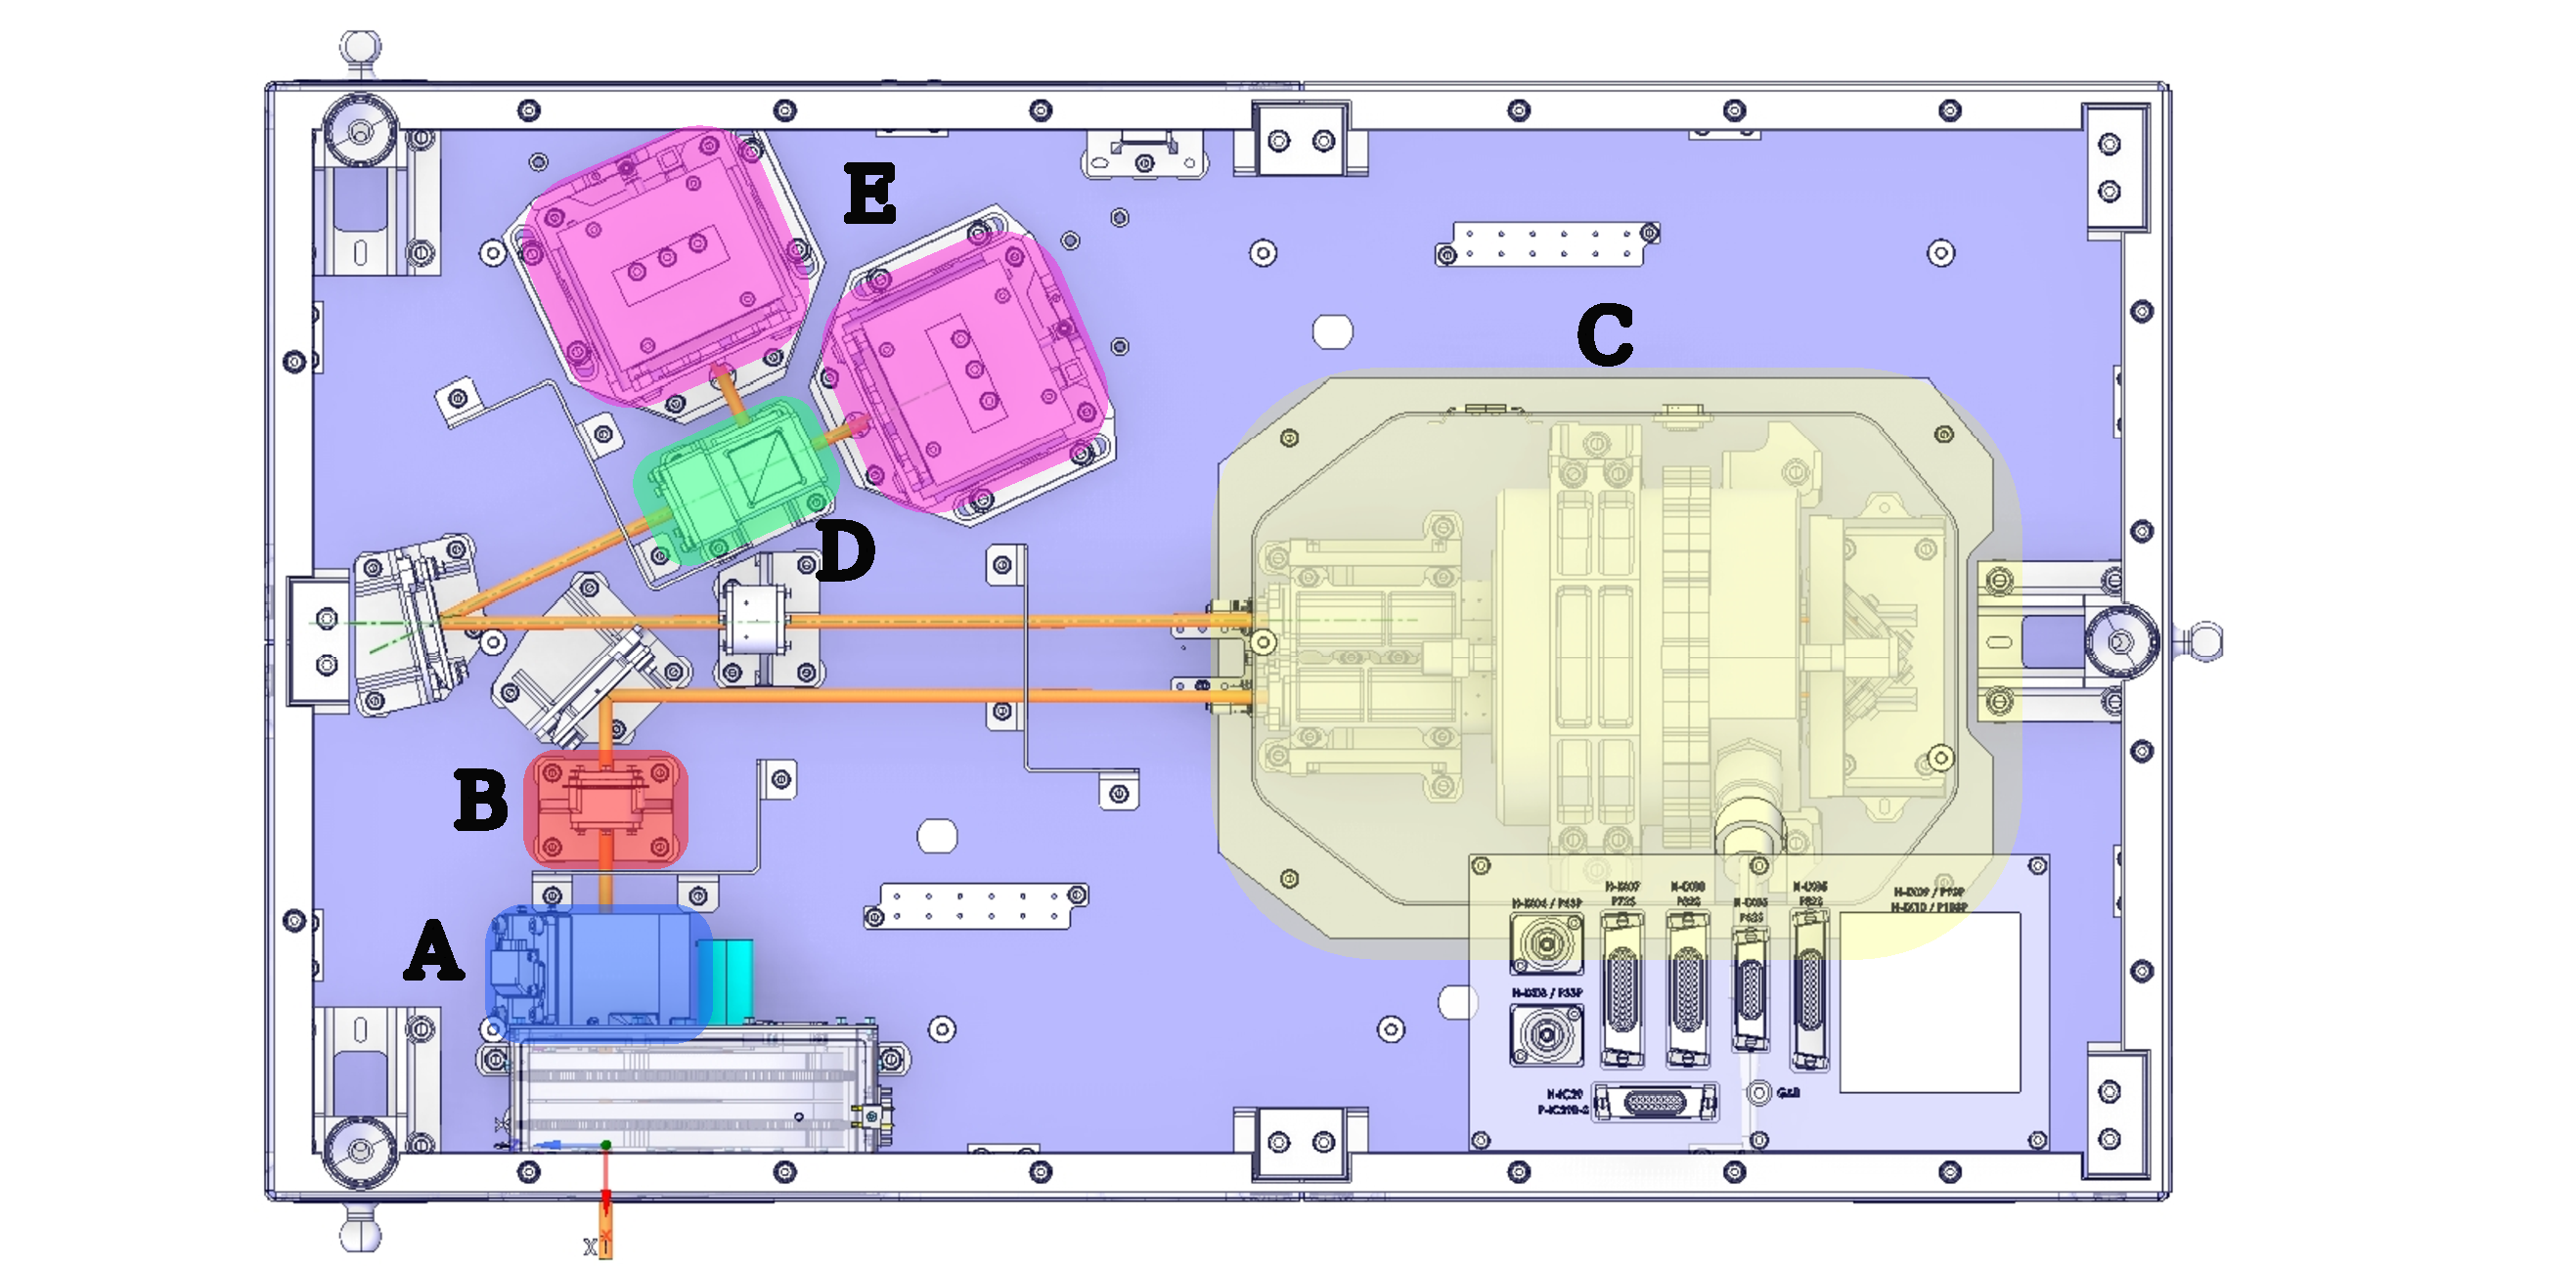
\includegraphics[width=\textwidth]{figures/TuMag/Scheme.pdf}
    \caption{Schematic representation of the Tumag instrument. Some relevant optical devices in the light path (yellow line) are highlighted with a colored box and labeled with leters from A to E: A) Filter wheel, B) PMP, C) Etalon oven, D) beam-splitter and E) cameras. Image taken from TUMAG PAPER REF, reproduced with permission.      
    \label{fig_tumag:scheme}}
\end{figure}

Light is delivered to TuMag by the ISLiD system and subsequently re-imaged onto two cameras where the images are recorded. Before reaching the cameras, the light passes through all the different subsystems of the optical unit. The first components encountered by the light are a blocking prefilter and the filter wheels (box A in Fig. ~\ref{fig_tumag:scheme}). The blocking prefilter, with a wide bandpass centered at 520 nm, is employed to eliminate unwanted spectral ranges. The filter wheels  are comprised by a double-disk system \citep{filter-wheels} that houses the prefilters for selecting specific spectral lines and a series of calibration modules. Specifically, three prefilters are mounted on the second disk of the filter wheel, corresponding to the spectral lines Fe I 5250.2 \r{A}, Fe I 5250.6 \r{A}, and Mg I $b_2$ 5172.7 \r{A}. Additionally, the filter wheels include a PD plate, which is used to introduce a known defocus into the final image to facilitate image reconstruction techniques, along with a linear polarizer, a plate of micropolarizers, and a pinhole set, employed during calibration observations.

After passing through the filter wheels, the light is directed into the Polarization Modulation Package (PMP), a subsystem derived from the SO/PHI instrument (\citealt{pmp1}, \citealt{PHI}), highlighted with the red box in Fig.\ref{fig_tumag:scheme}. The PMP's primary function is to modulate the light to produce the different polarization states required to deduce the Stokes components. This is achieved using two liquid crystal variable retarders (LCVRs), which are oriented with their fast axes at 45$^\circ$ relative to each other. These LCVRs induce a retardance on the transmitted light that varies with the voltage applied across the crystals. The system can operate in two distinct modulation schemes: a vector modulation scheme, which generates four independent linear combinations of equally-weighted Stokes components across consecutive observations, allowing for the retrieval of the full Stokes vector after demodulation; and a longitudinal modulation scheme, which generates only two modulations, providing information solely on the intensity and circular polarization.

Following modulation, the light is directed into a LiNbO$_3$ Fabry-Pérot etalon, highlighted in yellow in Fig.\ref{fig_tumag:scheme} (box C). Likewise IMaX, the etalon operates in a collimated setup and with a double pass configuration \citep{etalon-doublepass}. In this configuration, after the light passes through the etalon once, it is redirected by a pair of mirrors to pass through the etalon a second time. This double-pass configuration significantly enhances spectral resolution by narrowing the transmission profile. The LiNbO$_3$ etalon tunes the resonance wavelength by varying the refractive index of the cavity through the application of high voltages (ranging from $-4000$ V to $4000$ V) to the mirrors. Compared to air-gapped etalons, these kind of etalons offer the advantage of having no moving parts, which is particularly beneficial for spaceborne or balloon-borne instruments. However, this advantage comes with the need for precautions to prevent discharges caused by air ionization.

The final optical element the light encounters before reaching the cameras is a polarizing beam splitter (gree box C in Fig.\ref{fig_tumag:scheme}). At this stage, the light beam is divided into two orthogonal, linearly polarized components, each directed towards a different camera. This dual-beam configuration \citep{lites-doublebeam} is designed to minimize spurious signals induced by jitter of the gondola (see \cite{libro_JoseCarlos} for an extended discussion), as it effectively cancels fluctuations from Stokes I to the other Stokes parameters that may arise due to image motion or solar evolution (\textit{i.e.} cross-talk).

Light then reaches the cameras, shown with pink boxes (boxes E) in the scheme, where images from both are recorded and stored. After mission recovery, the data is processed on-ground to combine images from the different cameras, modulation states, and spectral lines, ultimately deriving the scientific products. This processing and reduction of the data is accomplished using software specifically developed for TuMag, which will be extensively discussed in Section XX. 

\section{Instrument performance and verification.}

All subsystems within the TuMag light path function collaboratively to deliver high-resolution spectroscopic data of the solar spectrum. To ensure data quality, TuMag underwent multiple verification and calibration processes, during which its spectral, polarimetric, and imaging properties were meticulously tested. These procedures, commonly referred to as end-to-end (E2E) calibration tests, were conducted at various stages of the mission. Specifically, they were performed during the assembly, integration, and verification (AIV) activities with the stand-alone instrument at INTA facilities in Madrid, Spain; during the AIV phase of the post-focus instrument (PFI) platform at MPS facilities in Göttingen, Germany; and during the TuMag AIV phase in the Sunrise III mission at ESRANGE facilities in Kiruna, Sweden. These tests were designed not only to validate the instrument's capabilities but also to measure critical parameters such as the tuning constant of the etalon, modulation matrices, and best-focus position—each of which is vital for the optimal operation of TuMag and the subsequent data processing (see \cite{e2e-tests-inta} for a detailed description of the tests). We will now delve into the details of the imaging, spectral and polarimetric properties of the instrument as well as the verification processes and results, as the two are intimately related.  

\subsection{Imaging performance.}
TuMag captures photons using two custom-made cameras \citep{tumag-cams} equipped with GPIXEL back-illuminated GSENSE400BSI detectors, each featuring a $2k \times 2k$ pixel array, and specifically designed to meet TuMag's scientific requirements. These cameras provide a broad FoV of $63'' \times 63''$, sufficient to encompass an entire medium-sized active region, with a plate scale of $0.0378''$/pixel.

In order to fulfill the requirement of the wavefront error of $W \sim \lambda / 14$, the instrument must have means to correct for the additional aberrations introduced by the telescope, the image stabilization and light distribution (ISLiD) system and uncorrected jittering. For this purpose, TuMag is equipped with a PD plate in the filter wheel that allows for the assesment of PSF during the observations to apply image restoration techniques during the data processing.  

The imaging E2E tests involved projecting several targets at the F4 focus, including a USAF test target, star targets, and a grid, observed both with and without the PD plate. These targets were utilized to evaluate the MTF and to assess the resolving power of TuMag. The PD measurements enabled verification of the wavefront error (WFE) derived from the MTF and an evaluation of the image quality following image restoration. 

The USAF target \footnote{The 1951 USAF target from Thorlabs Inc, model: R1DS1N.} consists on a series of horizontal and vertical line pairs (lp) aranged in sets of three with varying resolutions. Identifying the highest resolution group observable with TuMag allows for a fast diagnostic of the instrument resolution and performance. In fig.~\ref{tumag : USAF}, measurements of group 4 and 5 (and higher) of the USAF target are shown for both cameras and the three pre-filters. The set 2 of group 5 (highlighted in a white box), which corresponds to 35.9 lp/mm in the target and 24.3 lp/mm in the image, is of special interest since its close to the Airy disk radius (26.4 lp/mm) and therefore close to TuMag's resolution limit. 

\begin{figure}
    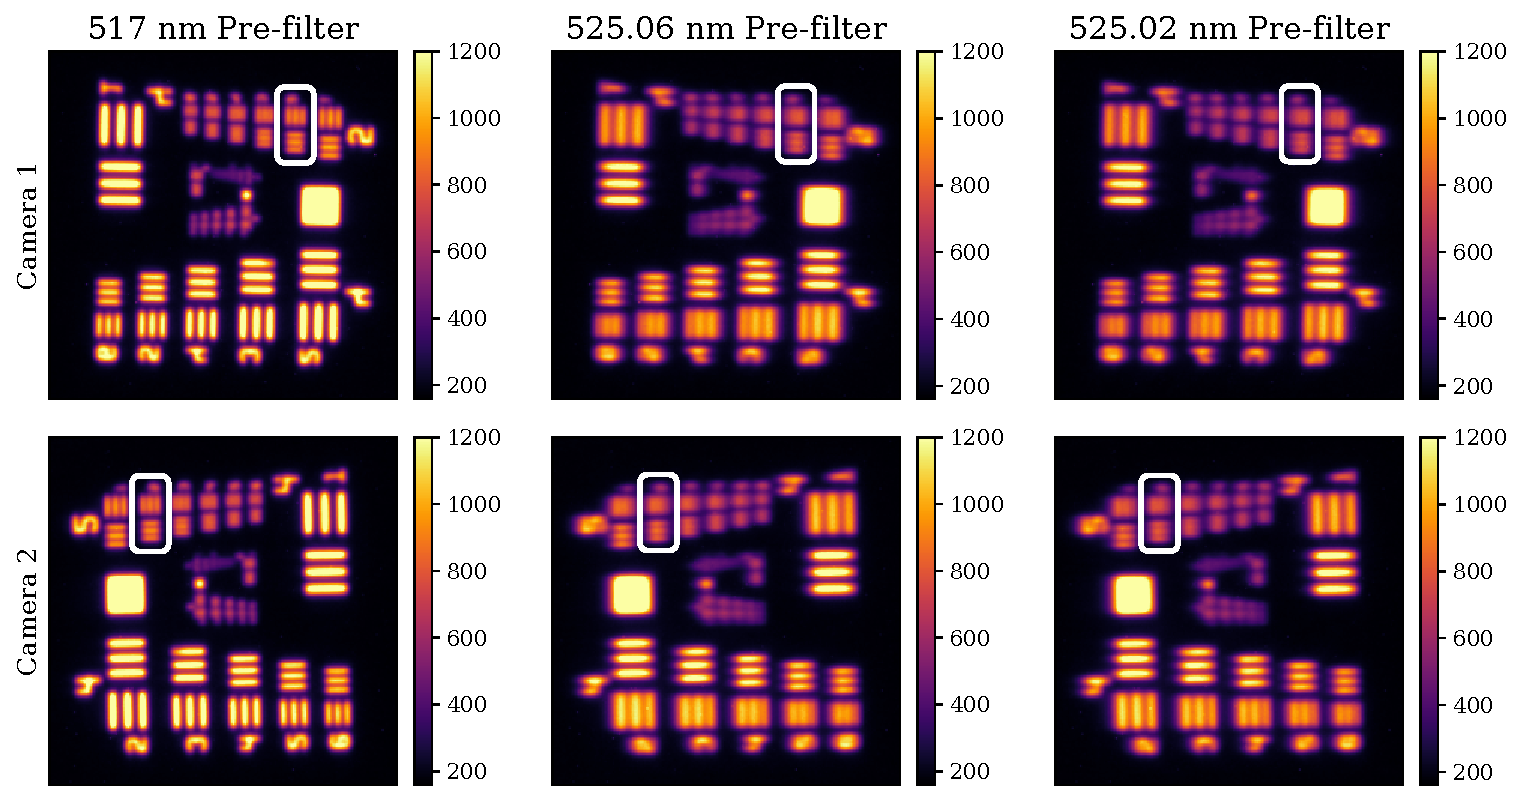
\includegraphics[width=\textwidth]{figures/TuMag/USAF_E2E.pdf}
    \caption{
      USAF target measurements for both cameras and the three pre-filters performed during E2E tests at INTA facilities on December 2021. The white boxes highlight the second element of the test group 5 (35.9 lp/mm). The scale of the images is set in digital counts.}
      \label{tumag : USAF}
\end{figure}

The results show a better optical performance for the 517 nm pre-filter than the other two pre-filters. The USAF 5.2 set is clearly resolved fo this pre-filter in both cameras showing almost no differene between vertical and hiorizontal resolutions. However, results for the 525 nm prefilters exhibit a worsening of the resolution, with the same set being hardly resolved in the horizontal direction in both prefilters. 

\begin{figure}
    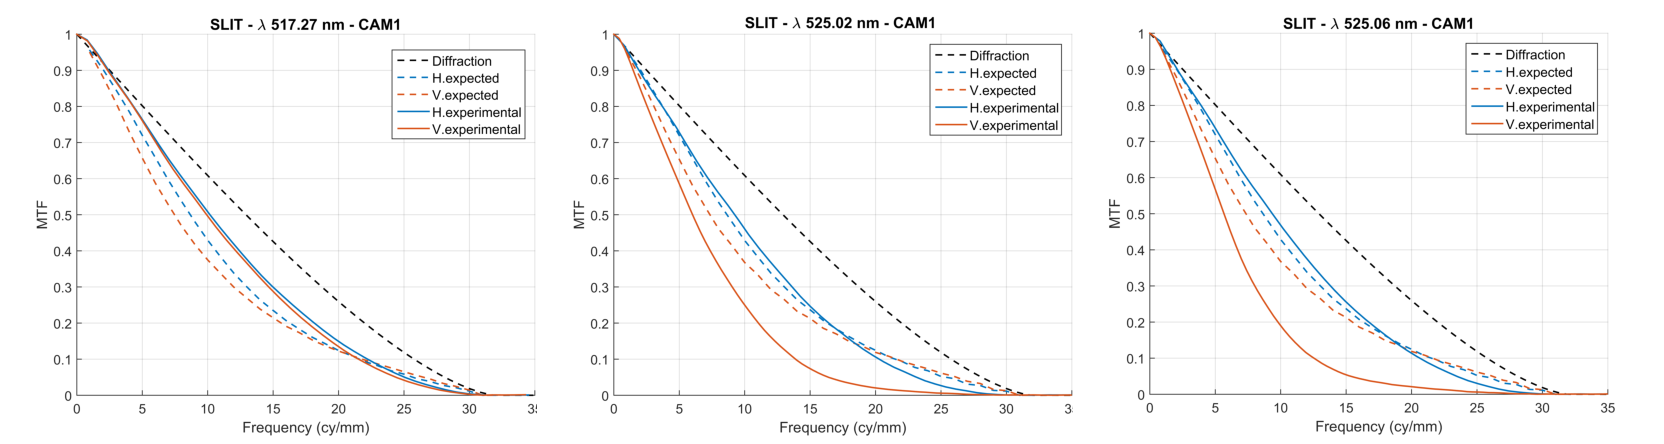
\includegraphics[width=\textwidth]{figures/TuMag/mtfs.pdf}
    \caption{MTFs derived for camera 1 (very similar results for camera 2) for the three pre-filters from measurements of the stand-alone AIV phase performed at INTA in December 2021.  
      \label{fig_tumag:mtfs}}
\end{figure}


However, a more precise evaluation of the optical performance can be achieved from the MTFs. Figure \ref{fig_tumag:mtfs} shows the MTFs computed with a slit target (see \cite{slanted-method} for a description of the MTF computation) during the E2E tests performed in December 2021 at INTA facilities. These results agree with the diagnostic carried with the USAF tests: the 517 nm pre-filter shows a good performance in both directions, with values above the expected behaviour. Meanwhile, 525 pre-flters exhibit a large difference between different directions with an important drop in vertical resolution in both cases. This observed astigmatism is attributed to the etalon and physical deformations of the pre-filters caused by the mechanical method used to secure and tilt them. This effect is particularly noticeable in the iron pre-filters due to the higher angles of incidence required for their tuning.

\begin{table}
    \centering
   \begin{tabular}{ccccc}
    \hline
    \hline
    Pre-filter and & Strehl ratio & Strehl ratio & WFE& WFE\\
    camera & Vertical & Horizontal & Vertical & Horizontal\\
    \hline
    517 nm - Cam 1 & 0.782 & 0.826 & $\lambda/12.7$ & $\lambda/14.5$ \\
    517 nm - Cam 2 & 0.761 & 0.806 & $\lambda/12.1$ & $\lambda/13.5$ \\
    525.02 nm - Cam 1 & 0.436 & 0.725 & $\lambda/6.9$ & $\lambda/11.1$ \\
    525.02 nm - Cam 2 & 0.405 & 0.726 & $\lambda/6.6$ & $\lambda/11.1$ \\
    525.06 nm - Cam 1 & 0.451 & 0.764 & $\lambda/7$ & $\lambda/12.1$ \\
    525.06 nm - Cam 2 & 0.444 & 0.736 & $\lambda/7$ & $\lambda/11.3$ \\
    \hline
    \hline
    \end{tabular}
    \caption{Optical performance evaluated from the MTFs obtained with the slit target at December 2021 E2E tests.}
    \label{table: Optical-performance}
\end{table}


The comparison of the obtained MTF and the difraction-limited one allows for an estimation of the Strehl ratio, and consequently the wavefront error (see section \ref{sec: intro-imaging}).

Table \ref{table: Optical-performance} shows the results for the Strehl ratios and WFE derived from this computation. All values, except for the horizontal resolution in camera 1 of the 517 nm prefiter are lower than the $\lambda/14$ set as a requirement. However, images can always be restored if $WFE \gtrapprox \lambda / 5$ \citep{restoration-limit} if the PSF is known, thus the need for the inclusion of PD capabilities in the instrument. Furthermore, PD techniques not only allow us to enhance the optical performance of the instrument but also evaluate the optical performance during the calibrations in order to verify the results obtained through the computation of the MTF. 

\begin{figure}
    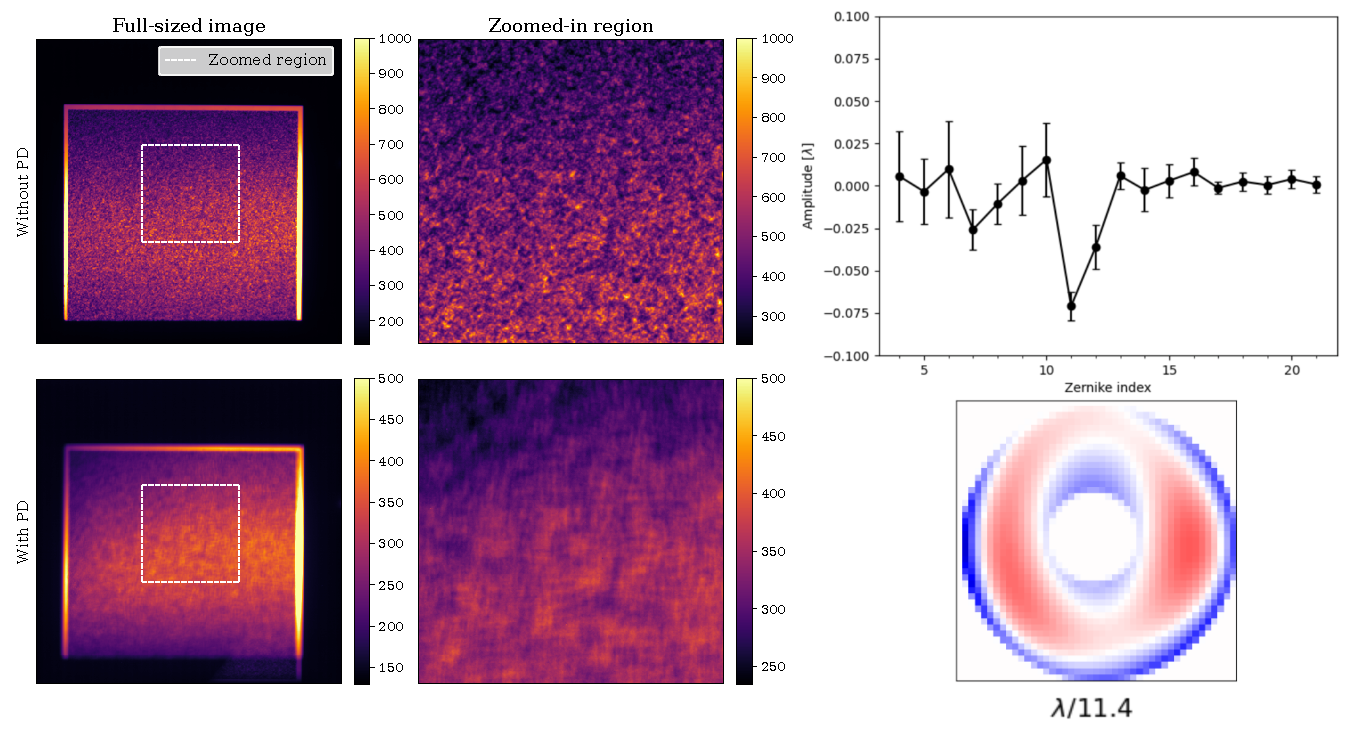
\includegraphics[width=\textwidth]{figures/TuMag/PD_e2e.pdf}
    \caption{Random dot target measurements of the 517 nm pre-filter with the camera 1 and without the PD plate (left and central columns) taken during the Sunrise III AIV phase in Kiruna on April 2024. The right column shows the Zernike coefficients obtained from the PD analysis in the top panel and the 2D representation of the rms WFE. The PD analysis has been carried out by F. J. Bailén, reproduced with permission.}
      \label{tumag : PD}
\end{figure}

Figure \ref{tumag : PD} shows the measurements and results of the PD analysis for the 517 nm pre-filter and the camera 1. The measurments were carried out during the final E2E tests performed at Kiruna on April 2024 using the random dot target (left and central columns of the figure). The measurements consist on 5 sets of focused-defocused pairs of images. The PD algorithm is run over a zoomed-in region of 600 pixels in sub-patches of 128x128 pixels. The mean Zernike coefficients are shown in the top right panel, where the error has been computed as the standard deviation between different sub-patches. A 2D representation of the rms WFE is also shown in the bottom right panel. 

The PD analysis indicates a small amplitude for most aberrations, with coefficients beyond Z15 approaching zero. Except for the spherical aberration ($Z_{11}$, $Z_4 ^0$) which is the dominant contribution to the rms wfe. However, the results exhibit significant dispersion, as reflected by error bars that reach values up to 0.025$\lambda$ for the first coefficients. Both the defocus and astigmatism are pretty low (Zernike indexes 4, 5 and 6, $Z _ 2 ^0$, $Z _ 2 ^{-2}$ and $Z _ 2 ^2$, respectively), agreeing with the results obtained from the MTF analysis which showed a good resolution in both vertical and horizontal directions. The overall rms WFE obtained from this analysis is $\lambda / 11.4$. It is important to note that the PD analysis and the modulation transfer function (MTF) determination were conducted at different stages of calibration, under varying conditions, which accounts for the observed differences. Nevertheless, both analyses agree on a WFE better than $\lambda / 10$, indicating very high optical quality, despite the fact that the FPIof TuMag operates in a collimated configuration, which is known to degrade optical performance \citep{ghosts-etalon}.

\subsection{Spectral performance.}

TuMag filters wavelengths through a sequential process, beginning with a broad blocking pre-filter that eliminates unwanted portions of the solar spectrum, and followed by a second narrow-band pre-filter that is tuned to the three selected spectral lines. Finally, the LiNbO$_3$ Fabry-Pérot etalon is encharged of selecting a very narrow band around specific wavelengths along the spectral lines. The narrow-band pre-filter and the etalon are critical to TuMag's spectroscopic performance and require careful evaluation during calibration.

The three TuMag pre-filters were custom-manufactured by Materion$^{TM}$ and have a full width at half maximum (FWHM) close to 1 nm. They are centered near the rest wavelength of the three spectral lines at normal incidence, with a peak transmission exceeding 80\% in all cases. Each pre-filter was tuned by adjusting the incidence angle to align the peak transmission wavelength with the spectral line core. This process was performed using a coelostat at the INTA facilities, where the rest positions in volts of the spectral lines were determined. The Fe I 5250.2 \r{A} line was found at 2129 V, the Fe I 5250.6 \r{A} line at -2507 V, and the Mg I $b_2$ 5172.7 \r{A} line at -2245 V. While this tuning was successful, particularly for the iron lines, the spectral position of the pre-filters was found to be highly sensitive to illumination conditions. This sensitivity was evident from the shifts observed in the pre-filter measurements during the various stages of the assembly process. As illustrated in the left column of Fig.~\ref{fig_tumag: spectroscopic_results}, the variation in the spectral position of the pre-filters is not sufficient to cause the spectral line to be blocked by the pre-filter, but it may result in the spectral line falling on the wing of the pre-filter during observations.

\begin{table}
    \centering
   \begin{tabular}{cc}
    \hline
    \hline
    Property & Value \\
    \hline
    Reflectivity & 0.892 \\
    Thickness & 281 $\mu$m\\
    FWHM (double-pass) & 0.8\\
    Tuning Constant & 3300 V/\r{A}\\
    \hline
    \hline
    \end{tabular}
    \caption{Tumag Fabry-Pérot specifications.}
    \label{table: Tumags etalon}
\end{table}

\begin{figure}
    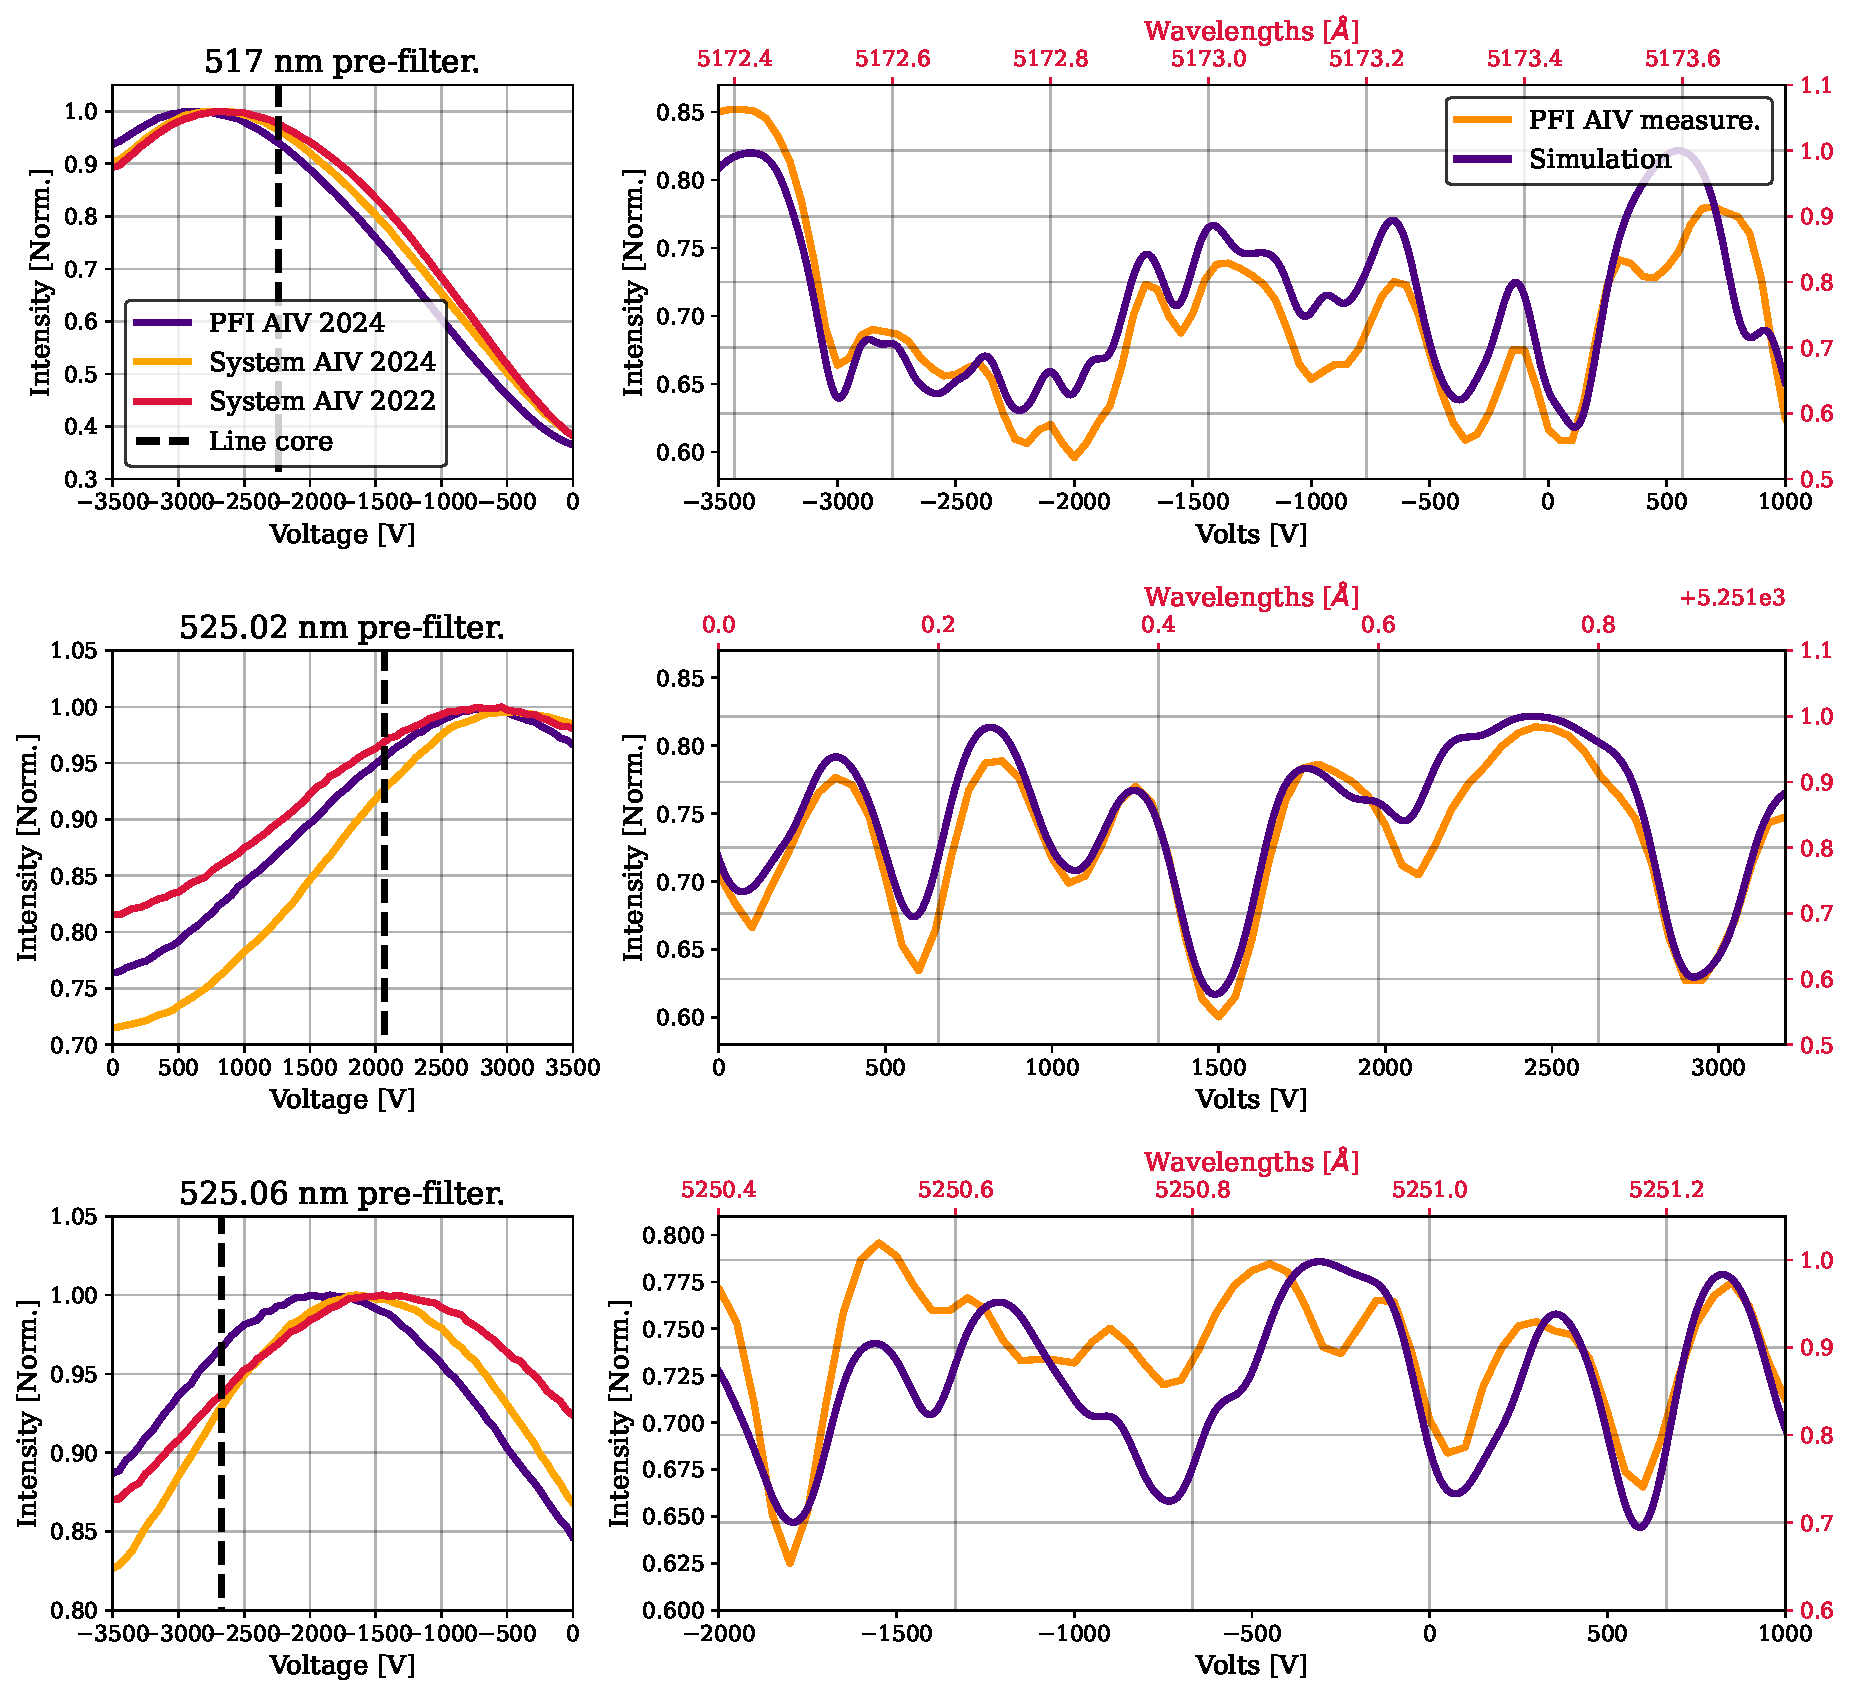
\includegraphics[width=\textwidth]{figures/TuMag/Spectroscopic_calibration.pdf}
    \caption{
      TuMag spectroscopic calibration results. Each row shows results for the 517 nm, 525.02 nm and 525.06 nm pre-filters, from top to row. The left column shows measurements of the pre-filters carried out with a flat LED on different stages of the AIV phases. The right column shows the fit of the I$_2$ cell observation with a simulation employing an etalon with a reflectivity of 0.892 (FWHM$\sim 0.87$). Note that the absolute value of the wavelengths of the simulation (red axis) might be shifted with respect to real values due to unknown conditions of the reference.   
      \label{fig_tumag: spectroscopic_results}}
\end{figure}

TuMag's etalon (see Table \ref{table: Tumags etalon}) operates in a collimated setup with a transmission profile with a FWHM of 0.87 pm (in the double-passs configuration), thus achieving a spectral resolution that exceeds the required 9 pm. Observations of an iodine cell illuminated with a diode were conducted to verify the transmission profile's shape and accurately assess the tuning constant. The right column of Fig.~\ref{fig_tumag: spectroscopic_results} presents, in orange, the iodine cell measurements obtained during the assembly, integration, and verification (AIV) phase of TuMag's integration into the Post Focal Instruments (PFI) platform, which took place at the Max Planck Institute for Solar System Research (MPS) in Göttingen, Germany, in November 2023. Additionally, the dark blue line in the figure represents a simulation of the iodine spectrum observations. This simulation was generated using an analytical model of the transmission profile of collimated etalons (see section \ref{susec_etalon_theory: collimated} for a detailed overview of the model). The results confirm that the spectral resolution achieved in the iodine cell observations is consistent with the estimated 0.87 pm resolution. Furthermore, these observations enabled the calculation of the etalon's tuning constant by identifying the corresponding line cores between the simulation and observation and applying a least squares fitting to establish the relationship, which was measured in 3300 V/\r{A}.

\begin{figure}
    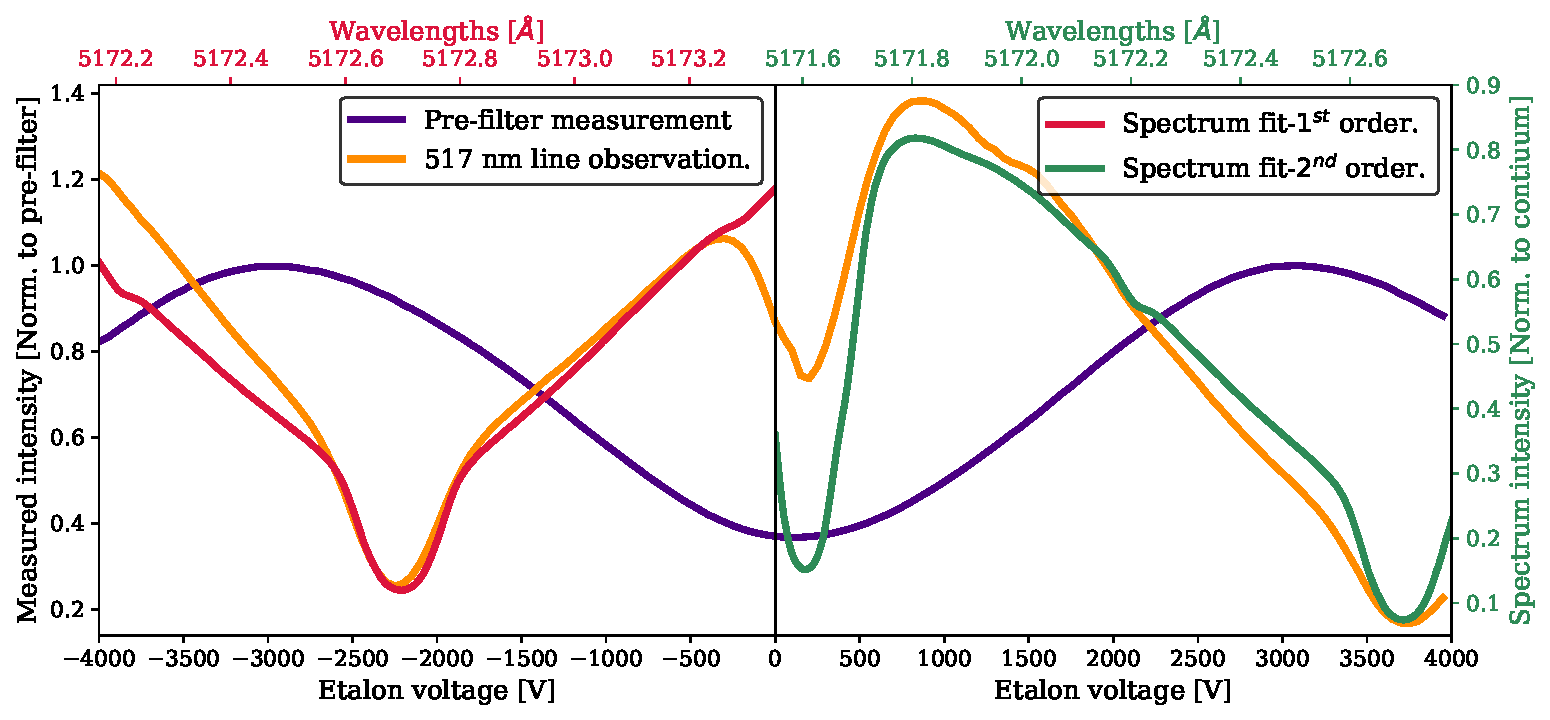
\includegraphics[width=\textwidth]{figures/TuMag/secondorder.pdf}
    \caption{
      Results of the spectroscopic calibration during the end-to-end calbrations of the AIV phase of 2021. The dark blue curve represents the measurement of the 517 nm pre-filter, alongside an observation of the magnesium line using the coelostat at INTA facilities, shown in orange. Two different fits of the solar spectrum are overplotted on the figure. The red line represents a fit to the primary etalon order (negtive voltages), while the green line corresponds to a fit to the second etalon order (positive voltages).      
      \label{fig_tumag:second-order_cont}}
\end{figure}

An observation of the solar spectrum with the 517 nm pre-filter, conducted at INTA facilities in December 2021 during the end-to-end calibration tests, is presented in Fig.~\ref{fig_tumag:second-order_cont}, along with the corresponding pre-filter measurement. The magnesium line core is detected at approximately -2200 V using the primary order of the etalon and reappears around 3750 V with a secondary order. A fitting of the solar spectrum\footnote{Reference} is also shown for both orders. These results reveal significant contamination from the secondary order near the pre-filter's minimum transmittance. At around 0 volts, the observed spectrum (orange line) is a composite of contributions from both the primary (red line) and secondary (green line) orders. This contamination is particularly relevant for data processing, as continuum measurements of the magnesium line are typically conducted at -80 V. The broader profile of the magnesium line necessitates continuum measurements farther from the line core, making it more susceptible to this contamination. In contrast, the narrower iron lines do not require such extensive offsets for continuum measurements and are thus less affected.

\subsection{\label{sect:intro polarimetric}Polarimetric performance.}

TuMag modulates the incoming light through a PMP composed of two anti-parallel LCVRs. These devices can modify the phase retardance induced to the light that goes through them by changing the alignment of their molecules when subject to a voltage potential. Their advantages for airborne instruments lie in their lightweight and compact design, the low voltage required for operation ([$0 - 10$]V), and their efficiency in producing either four linearly independent modulation states for full-Stokes polarimetry or only two states for measuring the longitudinal component of the magnetic field through Stokes V. This versatility is a specific advantage of LCVRs, not found in quarter-waveplate-based PMPs \citep{pmp-advantages}.

\begin{table}
    \centering
   \begin{tabular}{cc|cccc|cc}
    \hline
    \hline
     & & \multicolumn{4}{c}{Vectorial} & \multicolumn{2}{|c}{Longitudinal}  \\
     Spectral lines & Modulation & I1 & I2 & I3 & I4 & I1 & I2 \\
    \hline
    525 \& 517 nm & LCVR1 retardance  & 225$^\circ$  & 225 & 315$^\circ$ & 315$^\circ$ & 180$^\circ$  & 180$^\circ$\\
    525 \& 517 nm  & LCVR2 retardance  & 234.74$^\circ$ & 125.26$^\circ$ & 54.74$^\circ$ & 305.26$^\circ$ & 90$^\circ$ & 270$^\circ$ \\
    \hline
    525 nm & LCVR1 voltage & 2.291 & 2.533 & 1.992 & 1.947 & 2.761 & 2.761 \\
     & LCVR2 voltage & 2.375 & 3.360 & 6.433 & 2.016 & 4.723 & 2.186 \\
    \hline
    517 nm & LCVR1 voltage & 2.343 & 2.580 & 2.031 & 1.972 & 2.797 & 2.797\\
     & LCVR2 voltage & 2.371 & 3.416 & 6.548 & 2.051 & 4.77 & 2.206\\
    \hline
    \hline
    \end{tabular}
    \caption{Tumag LCVR retardances and corresponding voltages for both modulation schemes and the three pre-filters. Note that a single value is provided for both iron pre-filters.}
    \label{table: polarimetric configs}
\end{table}

TuMag's polarimetric measurement approach is divided into the two modulation schemes already mentioned: vectorial and longitudinal. In the vectorial scheme, four linearly independent modulation states are generated in rapid succession by the PMP, enabling the calculation of the full Stokes vector. Conversely, the longitudinal approach generates only two modulation states, providing information on just two components. This modulation is designed to compute Stokes V by determining the quantities $I\pm V$.

Both modulation schemes are required to operate under an optimal modulation scheme. Such a scheme is defined by a modulation matrix with the following polarimetric efficiencies: $\varepsilon _{opt} \geqslant [1, \frac{1}{\sqrt{3}}, \frac{1}{\sqrt{3}}, \frac{1}{\sqrt{3}}]$. The selected modulation scheme was based on the retardances outlined in Table \ref{table: polarimetric configs}. A thorough calibration of the liquid crystal variable retarders (LCVRs) was conducted to accurately determine the voltages necessary to produce the specified retardances \citep{fine-tunin}.

Considerations on the (S/N) are critical for ensuring the required polarimetric sensitivity. Achieving an S/N of $10^3$ in the Stokes measurements imposes a requirement of $S/N \approx 1200$  for each modulation measurement per camera. This calculation assumes near-optimal polarimetric performance, and takes into account the dual-beam polarimetry technique, which increases the S/N by a factor of $\sqrt{2}$ when combining data from the two cameras. A single shot of the cameras is insufficient to reach these S/N values, as the sensors do not have enough capacity in their electron wells. To address this, multiple exposures are captured and subsequently summed during each observation. This \textit{accumulation} strategy, extensively tested and employed in various polarimeters (e.g., \citealt{accs1}, \citealt{accs2}, \citealt{accs3}), has proven compatible with image reconstruction techniques \citep{accs-image1, accs-image2}. It allows for adjusting S/N levels depending on the scientific objectives of the observation, balancing between velocity and polarimetric sensitivity.

However, in order to fulfill the polarimetric sensitivity requirements, the modulation matrix of the instrument must be carefully addressed during the polarimetric calibrations. Any deviation in the computation of the modulation matrix, will introduce spurious signals in the polarization measurements, known as cross-talk. The polarimetric calibration involves a series of measurements using a light beam with a known polarization state, generated by a rotating linear polarizer and a rotating quarter-waveplate. By varying the positions of these two devices, 40 different input polarization states were produced and measured with three pre-filters. These measurements allowed for the precise determination of the modulation matrix by solving the system of equations \eqref{eq_intro:modultaion_eqs}, where the only unknown is the modulation matrix $\textbf{M}$, as both the measured modulation and the Stokes components of the incoming light are known.

The results of the polarimetric calibration performed during the end-to-end (E2E) tests at INTA in December 2021 are presented in Fig.~\ref{fig_tumag:pol eff maps}. The figure shows the results for camera one; however, camera two demonstrated nearly identical efficiencies. The polarimetric efficiencies across the entire field of view (FoV) exceed the required thresholds $\varepsilon _{req} \geqslant [0.95, 0.45, 0.45, 0.45]$, and approach the optimal values.


\begin{figure}
    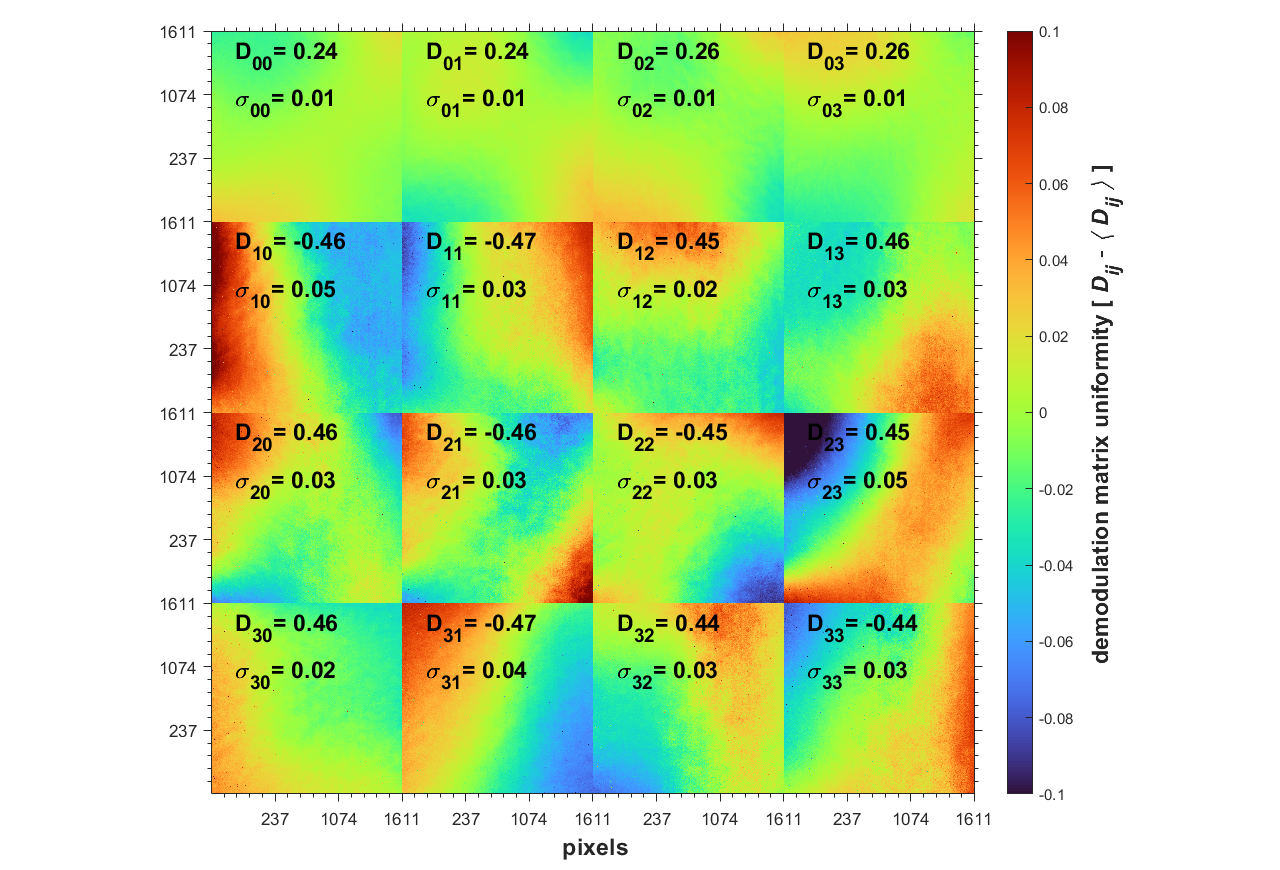
\includegraphics[width=\textwidth]{figures/TuMag/Pol_efficiencies_map.png}
    \caption{Polarimetric efficiencies for camera 1 and the three pre-filters (from top to bottom, the different rows show the results for 517 nm, 525.02 nm, and 525.06 nm). The different columns correspond to the efficiencies of the different Stokes components. The colormap measures the differences in efficiencies along the FoV. Results obtained during the E2E tests performed at INTA in December 2021, during the stand-alone AIV phase. 
    \label{fig_tumag:pol eff maps}}
\end{figure}



% Pipeline
%\chapter{\label{CH:Pipeline}TuMag's pipeline and data.}


The 2024 observational campaign of the third edition of the Sunrise observatory was an outstanding success. In contrast to previous flights, where technical challenges severely limited the number of useful observations, all subsystems performed exceptionally well during this third flight, allowing for nearly continuous instrument operation over more than six days. From TuMag’s perspective, the campaign yielded approximately 10 terabytes of data, consisting of over 40 scientific observation blocks and 250 calibration observations.

The substantial volume of data recorded by the three instruments, of which TuMag captured the least (in digital space) due to the instrument’s nature, required that it be physically recovered on-site, as it could not be broadcasted from the observatory to the operations center. Recovery activities began immediately after landing and lasted until early August, during which all surviving components, along with the data vaults, were transported to Yellowknife, Canada, the nearest city to the landing site. The data vaults arrived at MPS in early August, where a backup was created before the data associated with each instrument was sent to the respective IP institution. TuMag’s data arrived at  IAA in late August, marking the official start of the reduction process.

The reduction process began by labeling all images and identifying the more than 600 000 images captured by TuMag. Once the observations were correctly identified, the reduction process commenced and, at the time of writing, remains ongoing. Due to the relevance of the pipeline development and results for this thesis, this chapter will provide an overview of TuMag's data and the state of its pipleine, although the results remain preliminary.

The discussion will begin by introducing TuMag’s various observing modes, both scientific and calibration, followed by a brief review of the observation campaign, outlining the different observation programs and their scientific objectives. The chapter will conclude with an examination of the data reduction process, detailing the pipeline and presenting some initial results. It is important to note that, due to the late arrival of the data, this thesis had to be written in parallel with the reduction process. Therefore, the results presented here are preliminary, and the final product may differ as additional reduction steps are incorporated.

\section{TuMag's observing modes}

With the purpose of simplifying the operation activities, TuMag operates through a series of so-called observing modes. The observing modes are a list of pre-configured settings tailored for various observations, including both calibration and scientific purposes. Each mode is designed to fulfill the specific objectives of the corresponding observation and enables nearly automatic operation of the instrument during flight.

\begin{table}
    \centering
   \begin{tabular}{cccccccc}
    \hline
    \hline
    Observing mode & Spectral lines  & $N_\lambda$ & $N_P$ & $N_a$& $N_c$ & $t_{eff} (s)$ & (S/N) \\
    \hline
    0s & Mg I $b_2$ 5172.7 \r{A} & 12 & 1 & 2 & 1 & 6.3 & 500\\ 
    0p & Mg I $b_2$ 5172.7 \r{A} & 12 & 4 & 16 & 1 & 37.62 & 1000\\
    1  & Mg I $b_2$ 5172.7 \r{A} &  10 & 4 & 16 & 1 & 31.81 & 1000\\
    2  & Fe I 5250.2 \r{A}, Fe I 5250.6 \r{A} &  8 & 4 & 16 & 1 & 23.4 & 1000\\
    3  & Fe I 5250.2 \r{A}, Fe I 5250.6 \r{A} & 5 & 2 & 20 & 1 & 10.04 & 1000\\
    4  & Mg I $b_2$ 5172.7 \r{A} & 3 & 4 & 10 & 10 & 54.01 & 2500\\
    5  & Fe I 5250.2 \r{A}, Fe I 5250.6 \r{A} & 3 & 4 & 10 & 10 & 53.60 & 2500\\ 
    \hline
    \hline
    \end{tabular}
    \caption{Scientific observing modes. From left to righ, the columns are: observing mode identiicator, measured spectral lines, number of wavelengths, of modulations, of accumulations, of cycles, the total timeand the polarimetric SNR.}
    \label{table: scientific observing modes}
\end{table}

A summary of the properties for each observing mode is provided in Table \ref{table: scientific observing modes}. There are four distinct modes designed to observe the magnesium line. Mode 0s performs a fast, extended scan of the spectral line using 12 wavelength samples: [-40, -30, -20, -10, 0, 10, 20, 30, 40, 50, 60, 65]\footnote{Sampling positions are given relative to the line core.}, with one modulation and two accumulations to maximize scanning speed. Mode 0p is similar to mode 0s but employs a full-vector modulation scheme, requiring 16 accumulations to ensure the required SNR. Mode 1 provides a shortened scan of the magnesium line, with measurements taken at [-30, -20, -10, -5, 0, 5, 10, 20, 30, 65], also utilizing a vectorial modulation scheme. Finally, mode 4 is a "deep" magnetic mode, featuring a highly reduced scan with only three samples at [-10, 0, 10], but with increased accumulations and cycles to enhance polarimetric sensitivity. 

Three observing modes are configured for the iron lines. Mode 2 employs a vectorial modulation scheme applicable to both iron lines, with sampling at [-12, -8, -4, 0, 4, 8, 12, 22] pm. Mode 3 uses a longitudinal modulation scheme, measuring only Stokes I and V, with samples taken at [-8, -4, 4, 8, 22] pm. Lastly, mode 5 closely resembles mode 4, but is configured for the iron lines, with sampling at [-8, 0, 8] pm. The only difference between these two modes is the sampling scheme.

Although most of the parameters are set up by the observing mode and cannot be changed, there are some configurable parameters that allow to slightly modify the observing modes to fit the specific goal of a particular. These parameters are the following:

Solo estos? o había más? 
\begin{itemize}
    \Myitem $\lambda _ {\text{rep}}$ : A parameter that allows to repeat all the observations carried out at every spectral position before changing wavelength. This parameter is employed for flat-field observations (see the following section). By default is set to 1.
    \Myitem Etalon offset : A parameter that allows for the introduction of a global shift to the spectral sampling by offsetting the absolute voltages (and thus, wavelengths) of the scan. This parameter was used to center the spectral line in shorter observing modes affected by solar rotation or other effects that might shift the spectral position. The default value is set to 0 V.
    \Myitem $N_a$ : Even though the number of accumulations is fixed in nominal observing modes, this parameter was set as configurable in order to allow modifications for faster observations when needed. The  default value depends on the observing mode.  
\end{itemize}



\begin{figure}[t]
    \begin{minipage}[c]{0.67\textwidth}
      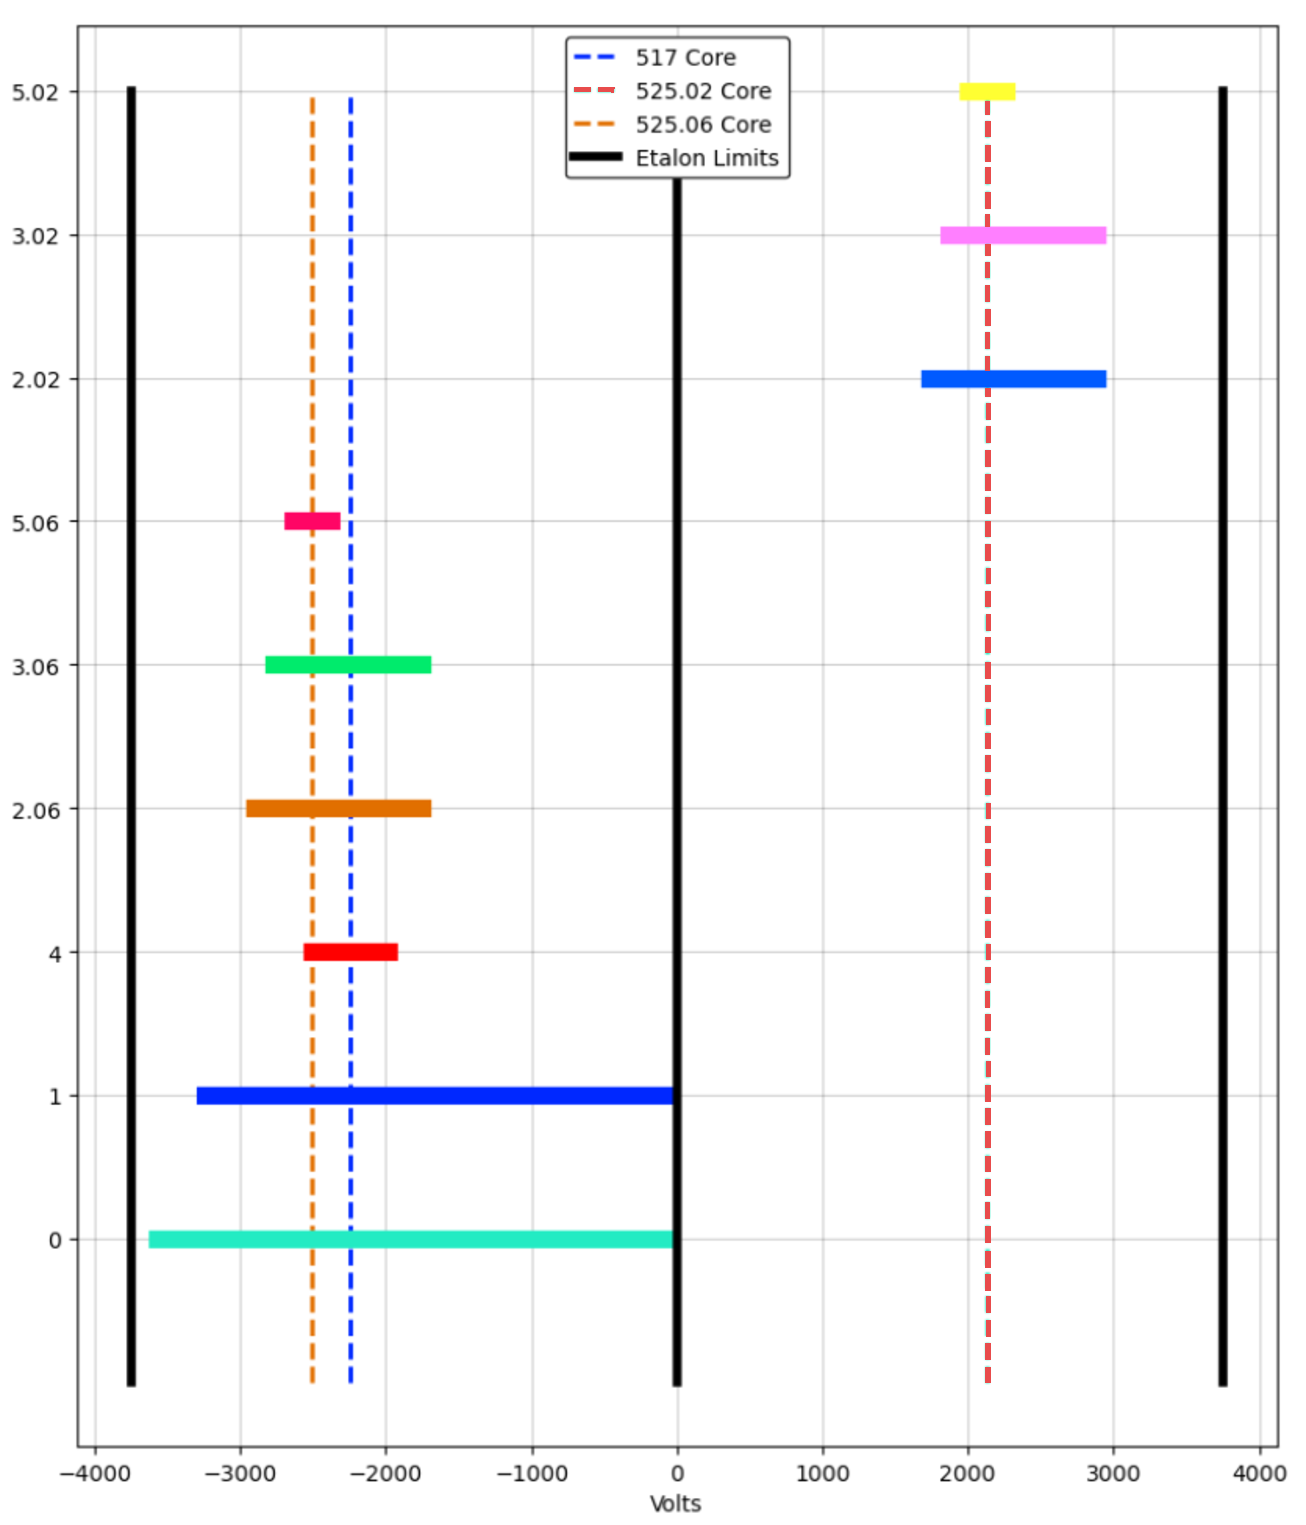
\includegraphics[width=\textwidth]{figures/Pipeline/obs_modes.pdf}
    \end{minipage}\hfill
    \begin{minipage}[c]{0.29\textwidth}
      \caption{
       Schematic representation of the voltage range covered by all observing modes. The dashed lines indicate the position of the line core as measured during the E2E tests performed at INTA in December 2021. The black lines represent the voltage limits that cannot be crossed in an observing mode.
       \label{fig_pipeline: Observing modes ranges}
      } 
    \end{minipage}
\end{figure}

Figure \ref{fig_pipeline: Observing modes ranges} presents a schematic representation of the voltage ranges for the observing modes when converting spectral sampling to volts. The black lines indicate the voltage boundaries that cannot be surpassed during an observation due to technical constraints. These limits are set at $\pm 3750$ V as the maximum and minimum values, with an additional limitation at 0 V, since a polarity change poses technical challenges that could not be addressed within an observation mode. These restrictions are significant in two cases: firstly, for Magnesium observation modes, specifically modes 1 and 0, where the continuum measurement is positioned as far from the core as possible, at -80 V, due to the 0 V crossing limitation. Secondly, these constraints are relevant when applying an etalon offset to shift the spectral positions of a particular observing mode, as the offset cannot cause the final positions to exceed these boundaries.

\subsection{Calibration modes}
An additional type of observing modes are also designed aimed at carrying out calibration observations. These calibration observing modes are more flexible than scientific ones, and allow for the configuration of several parameters to match the observations to the aim of the scientific observation. 

\begin{figure}[t]
    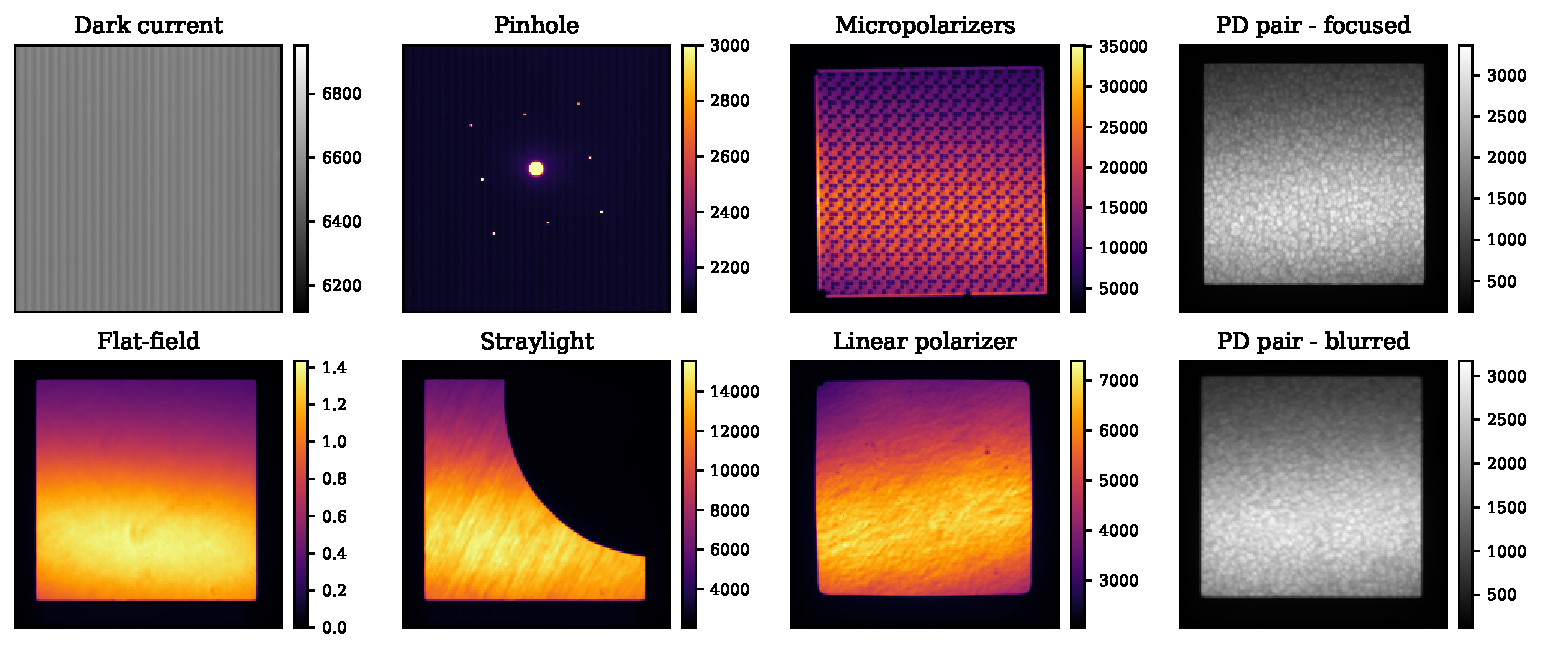
\includegraphics[width=\textwidth]{figures/Pipeline/cal_modes_examples.pdf}
    \caption{
      Examples of calibration observations. All images, with the exception of the flat-field, are presented in their raw format, without any manipulation or correction applied. The flat-field observation depicted corresponds to the first modulation of the continuum measurement obtained during a flat-field observation corresponding to observing mode 1. All data are belong to camera 1, and the colorbar is calibrated in digital counts save for the flat-field which is normalized to its mean value. }
      \label{fig_pipeline: cal_examples}
\end{figure}

\subsubsection{Flat-field observations}

One of the essential calibration procedures in any telescope-based astronomical observation is the acquisition of flat-field images. These observations are designed to measure intensity variations across the FoV, which arise from several factors, including intensity gradients induced by the etalon, dust particles, or pixel efficiency variations, among other sources. The aim is to capture a region with no discernible structure, ideally producing a uniformly flat intensity distribution. However, achieving such flat-field observations is not always straightforward, particularly for certain instruments. While ground-based telescopes can utilize twilight periods to observe areas of the sky devoid of stars, space-borne or balloon-borne solar telescopes, such as Sunrise III, are unable to the dame and must look for alternative methods. 

In Sunrise III, flat-field images are generated by deliberately blurring the solar image through rapid movements of the mirror. This process effectively removes any solar structure from the FoV when averaging out multiple blurred observations, resulting in a flat-field image devoid of solar features.

In the case of TuMag, flat-field observations are performed using a modified version of the nominal observing mode, where the $\lambda_{\text{rep}}$ is set to 4. Additionally, multiple consecutive instances ($N_{\text{reps}}$) of these observations are executed, typically 5 or 7. During data processing, a single flat-field is generated for each wavelength position and modulation state by averaging all corresponding observations.

Figure \ref{fig_pipeline: cal_examples} shows an example of a flat-field observation, for one camera, modulation and wavelength (bottom left panel). The image shows a clear deviation from flatness in the measurment, primarly due to the etalon intensity gradient, which accounts for the change in intensity between the brighter bottom half and the darker top half, and some minor inhomogeneities over the FoV. 

\subsubsection{Dark-current observations}

A second critical calibration procedure for any observation involving electronic cameras is the measurement of dark current. In the absence of incident photons, electrons within the camera's wells can still be randomly excited. This spontaneous excitation can be incorrectly interpreted as photon-induced counts when analyzing the data. Dark current observations are designed to characterize these random electronic excitations, which are primarily influenced by the camera's physical conditions, particularly temperature, so that they can be accurately subtracted from the final images.

For TuMag, dark current calibration involved capturing a series of 50 images with $N_a = 50$ with no light entering the instrument. As with flat-field observations, a single dark current frame for each camera is generated by averaging all individual observations. In the top left panel of fig. \ref{fig_pipeline: cal_examples} a dark current shot is depicted, characterized by the vertical strips pattern.  

\subsubsection{Linear polarizer and micropolarizers observations.}

TuMag's filter wheels are equipped with two targets designed to assess the instrument's polarimetric performance: a linear polarizer and a set of micropolarizers. Both targets are situated in the first filter wheel and are used in conjunction with the three distinct prefilters located in the second filter wheel. The linear polarizer serves to evaluate the polarimetric calibration, particularly by quantifying the level of cross-talk, as no circular polarization should be detected when using this target. The micropolarizers provide a more complete assessment, as they consist of multiple linear polarizers oriented at different angles. 

Observations with this targets are carried with the three prefilters, at a single wavelength, located in the continuum of each line. For each measurement, a vectorial modulation scheme is employed that allows for the derivation of the four stokes parameters. In the third column of figure \ref{fig_pipeline: cal_examples} observations of both targets are shown. 

\subsubsection{Pinhole Observations.}

Another calibration target included in the filter wheels is the pinhole target. This target blocks most of the light reaching the instrument, except for a few small holes arranged in a square-like pattern across the FoV, as shown in the top panel of the second column of figure \ref{fig_pipeline: cal_examples}. A larger hole is located at the center of the FoV, surrounded by eight smaller holes that trace a square with the central hole at its midpoint. These observations serve various purposes, including image alignment, detecting the presence of ghost images, or identifying etalon reflections, among other uses.

Pinhole observations are conducted similarly to those with polarizers, that is, in combination with the three prefilters at a single wavelength (the continuum of each line), but without applying any modulation.

\subsubsection{Straylight target.}

Not all the light that reaches the detector is necessarily the intended signal for a given observation. Some unwanted light, primarily originating from internal reflections along the optical path, may also reach the instrument. This unwanted contribution, known as straylight, contaminates the measurements by reducing contrast, lowering the S/N, and generally degrading the spectral, optical, and polarimetric performance of the instrument.

To address this contamination, TuMag performed a series of observations using a target that blocks part of the FoV (see the bottom panel of the second column of figure \ref{fig_pipeline: cal_examples}). By analyzing the dark region in these observations, it becomes possible to measure and model the straylight reaching the instrument, allowing for its subsequent removal from the data.

\subsubsection{Prefilter scans.}

TuMag observations are very sensible to spectral shifts either from the pre-filters or from the observed spectral line position. The shift of the pre-filters can happen due to changes in the physical conditions of the filter wheels such as changes in temperatures which spectraly shift the behavior of the pre-fitlers. The position of the pre-filter greatly affect the measurements as it reduces the intensity of the measurements that are obtained in the wings of the pre-filter. Due to solar rotation, or changes in the conditions of the etalon, although these are less likely, the spectral position at which the spectral lines are recorded can change. This effect is specially important in observing modes that require great spectral accuracy, such as the deep modes, where only three spectral positions close to the line core are employed. 

In order to verify the spectral behaviour of the prefilter, as well as the position of the spectral line, a series of observations were carried out, usually before and after the scientific observations, where a spectral scan with a rich spectral smapling was taken for all the pre-filters employed in the observation. These scans, measure the voltage range of the specific line with a sampling of 100V and without modulating. 

\begin{figure}[t]
    \begin{minipage}[c]{0.67\textwidth}
      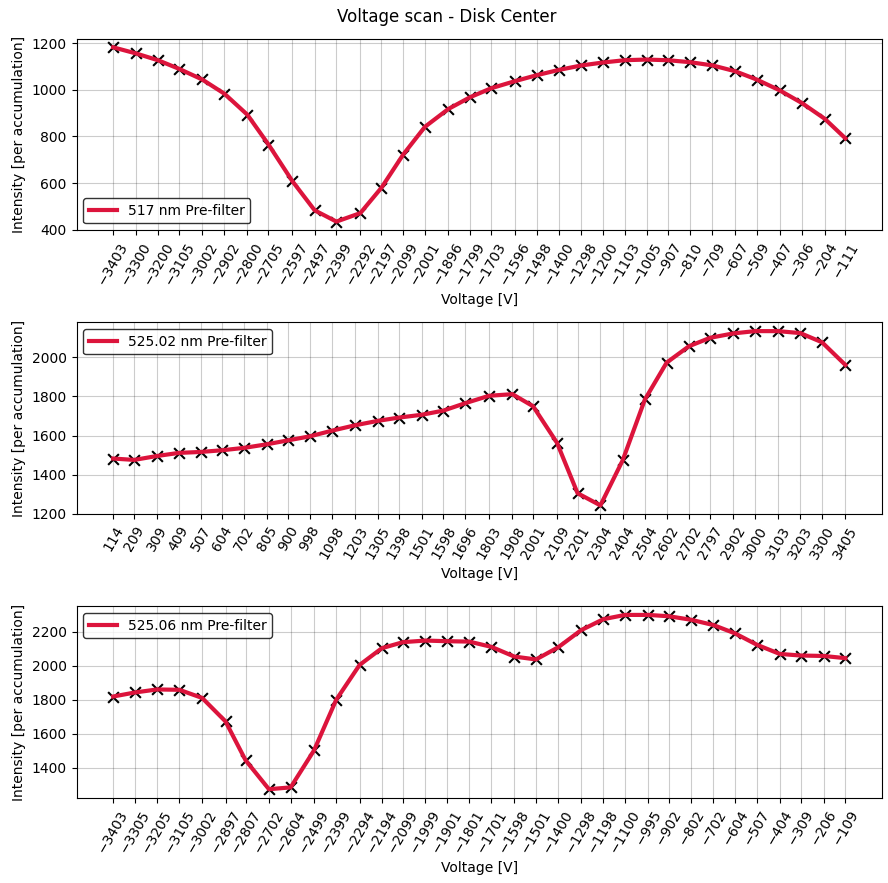
\includegraphics[width=\textwidth]{figures/Pipeline/Prefilter_scans.png}
    \end{minipage}\hfill
    \begin{minipage}[c]{0.29\textwidth}
      \caption{
       Schematic representation of the voltage range covered by all observing modes. The dashed lines indicate the position of the line core as measured during the E2E tests performed at INTA in December 2021. The black lines represent the voltage limits that cannot be crossed in an observing mode.
       \label{fig_pipeline:  prefilter_scans}
      } 
    \end{minipage}
  \end{figure}


\subsubsection{Phase diversity.}

Lastly, TuMag is equipped with the capability to perform phase diversity for image reconstruction. As discussed in previous chapters, applying image reconstruction techniques is essential to meet the optical quality requirements. To this end, TuMag includes a PD plate in the first filter wheel that introduces a known defocus in the images. Capturing images with and without this plate enables the computation of the instrument's PSF, which can then be deconvolved from the data.

PD measurements require quasi-simultaneous pairs of aberrated and unaberrated images. Therefore, TuMag's PD observations consist of a series of 32 or 40 rapid, non-accumulated shots with the PD plate, followed by a corresponding series without the PD plate. The feasibility of this sequential scheme for phase diversity techniques has been confirmed in \cite{PD_sequential}. A pair of focused-defocused images of quiet-sun observations is shown in the last column of figure \ref{fig_pipeline: cal_examples}.

\section{Timelines}

The operations of Sunrise III were designed to be nearly autonomous to ensure synchronization between the scientific instruments, the telescope, and the CWS. Given the limited time available for the observation campaign, this autonomy also helps to speed up operations, thus enabling more observation programs to be accommodated within the mission's duration.

The Sun is a highly dynamic system, exhibiting a wide range of behaviors and phenomena, from large-scale structures such as active regions, sunspots, and flares, to smaller, quiet Sun structures where interactions at small scales drive the evolution of magnetic flux. This diversity, observable in various spectral lines and across different regions of the solar disk, demands multiple observations with distinct characteristics.

Prior to the first flight of Sunrise III in 2022, a series of timelines were developed to program both calibration and scientific observation blocks. These timelines were carefully designed by the Sunrise Science Team, taking into account the 70 observing proposals submitted for Sunrise, in order to prioritize observations that met the requirements of the majority of these proposals.

Observing proposals that could be fulfilled by targeting the same solar feature, while considering its disk position, were grouped into a single timeline. Each timeline included not only the necessary scientific observation blocks but also the required calibration observations to ensure data accuracy. Thus, timelines consist of a sequence of scientific and calibration observation blocks. The observing blocks within a timeline could vary in content depending on the scientific objectives and the status of the other instruments involved.

For simplicity, operations related to SCIP and SUSI will be excluded from the discussion, save for a few important remarks. In the case of TuMag, each observing block was composed either of a combination of two observing modes executed consecutively, or a single observing mode repeated throughout the block.  

\begin{figure}
  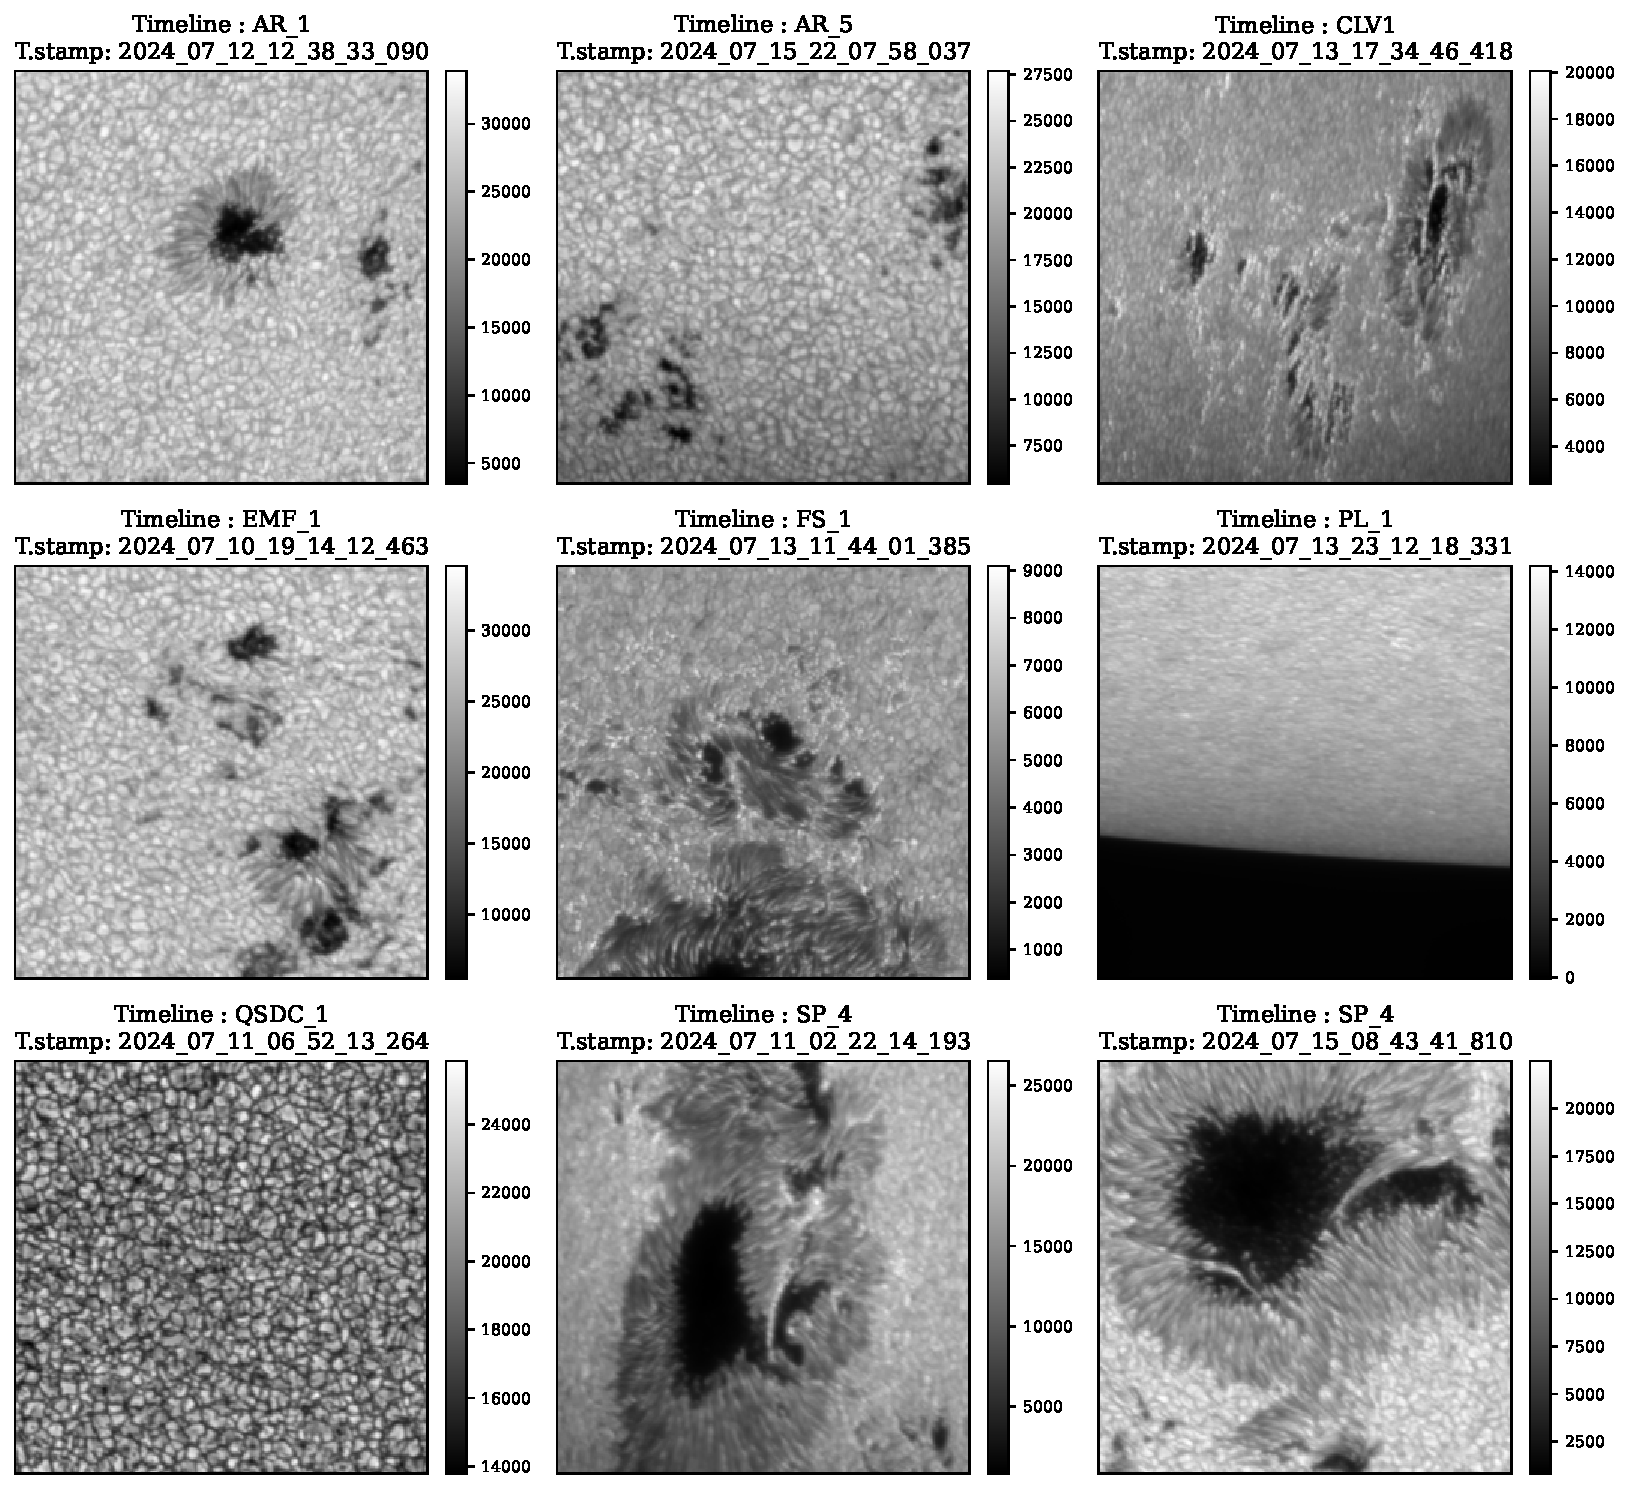
\includegraphics[width=\textwidth]{figures/Pipeline/timelines_Examples.pdf}
  \caption{
    Continuum images of the first modulation of the first observation mode from different timelines. The image shown has been flat-fielded and dark-corrected. The timestamp provided corresponds to the first image of the observation mode. The colorbar is given in counts.}
    \label{fig_pipeline: timeline_examples}
\end{figure}

The timelines of the Sunrise III observation campaign can be gropued in the following blocks: 

\begin{itemize}
  \Myitem Quiet Sun observations at disk center (QSDC), as the name implies , focus in regions near the solar disk center that are free from significant solar activity. These timelines typically involvve long series of observations aimed at studying the small-scale structure and magnetic flux evolution in the quiet Sun. 
  
  There are four distinct timelines in this category: three standard timelines, which ewmploy the nominal observing modes, and a different timeline, the (QSDC{\_}HC). This timeline employs high-cadence variations of the standard observing modes specifically designed to enhance the temporal resolution between images, which is crucial for helioseismology techniques.
  \Myitem Sunspot observations (SP) are specifically designed to study sunspots. There are four different timelines for this purpose. Some of these are short programs used to track the same sunspot over multiple days, with the goal of studying the evolution and decay of the sunspot. Others are more extensive programs aimed at examining, in greater detail, the magnetic activity of sunspots and their penumbral structures.
  \Myitem Polar observations (PL) target the region close to the limb in both poles of the Sun. These areas are of special interest due to their distinct magnetic behavior compared to the disk center. Additionally, these regions provide the opportunity to measure faint signals outside the main solar disk, such as spicules in the lower chromosphere, observed outside the continuum disk of iron. Two different instances of these timelines are conceived in the observation campaign, mostly differenciated in TuMag by the selected spectral lines.
  \Myitem East and West limb (EW) observations are designed to target the equatorial regions of the solar limb. In addition to exhibiting magnetic structures distinctly different from those observed at the poles, the reason for having a separate timeline from the PL timelines lies in the orientation and technical constraints related to SCIP and SUSI's slits. The relative positioning of the regions and the inclination of the telescope introduce unique challenges. In these EW observations, the spectrometer slits are aligned parallel to the limb, contrasting with the PL timelines, where the slit is positioned perpendicular to the limb.
  \Myitem Active regions (AR) observations are designed to study areas exhibiting solar activity, excluding those specifically focused on in the sunspot programs. These observations typically consist of two-hour series, employing the standard combination of the iron 525.02 nm and magnesium lines, using modes 1 and 2.02, which represent the most common observation block for TuMag. Although five different AR timelines were planned for the Sunrise campaign, only three were executed.
  \Myitem Emergence flux (EMF) programs are specifically desinged to study active regions that exhibit a large flux emercence. For TuMag, the observation blocks are shared with those of a the AR programs, namely, the combination of mode 1 and 2.02 for series of around 2 hours. 
  \Myitem Full spectral scan (FS) observations are primarily designed for SUSI and SCIP, where their complete set of spectral bands is utilized. These scans are intended to be carried out in both quiet Sun and active regions. For TuMag, FS observations consist of long series focusing on the iron spectral line in quiet Sun regions, while in active regions, they include a combination of iron and magnesium observations.
  \Myitem The flares programs (FL) were designed for target oportunities of a flaring region. These programs were intended to be activated only when an active region showed signs of flaring. For TuMag, the observations during these programs consist of the standard combination of iron 525.02 nm and magnesium spectral lines.
  \Myitem Center-to-limb variation (CLV) observations were intended to target regions of the solar disk characterized by $\mu$ values that had not been previously observed. The parameter $\mu$, defined as the cosine of the angle between the surface normal and the observer's line of sight, serves as a useful indicator of a region's proximity to the disk center. Specifically, $\mu$ ranges from 1 at the disk center to 0 at the limb \citep{thompson2006coordinate}. Conducting CLV observations at previously unmeasured $\mu$ values enables us to capture data from different regions across the disk, facilitating studies of how observational features vary with their position on the disk. 
\end{itemize}

During the Sunrise III observation campaign, 38 timelines were run, including calibration timelines in addition to the scientific programs presented here. Some examples of the different targets employed during the campaign are shown in fig. \ref{fig_pipeline: timeline_examples}.  A detailed record of TuMag's observations can be found online both in the pipeline's repository and in TuMag's official data website\footnote{\url{https://www.uv.es/jublanro/tumag_data_test.html}}.  

\section{Pipeline}

Before data can be employed for scientific purposes, it has to undergo a process where all the instrumental and spurious effects are removed and the necessary computations for the scientific aim are carried out. This process, usually refered to as data reduction, has to be specifically designed for each instrument, as the particular properties of the instrument come into play. Being a spectropolarimeter, TuMag's data reduction pipeline must, in addition to removing the instrumental artifacts, compute the stokes components of the incoming light.

In this section we introduce the software that has been developed for TuMag's data processing. Due to the proximity of the data's arrival to the end of this thesis, its important to note that the data reduction is still in development, with some calibration steps still undeveloped. In the following, we present the current status of the pipeline, along with a few examples of the results. The pipeline is publicly available in a GitHub repository\footnote{\url{https://github.com/PabloSGN/TuMags_Reduction_Pipeline}}.  

\subsection{Standard data reduccion process.}

The specific steps that have to be applied to a particular observation depends on the observation mode, and scientific aim of the observation, as different observations may require additional steps prior to the sicientific exploitation. However, any observing mode thats empoys either two of the modulation schemes, share a series of common steps that must be followed. Taking into account that save for the high cadence timelines, and the observing mode 0s, all observations follow this scheme, this is the process that the majority of TuMag data has to undergo. 

These steps include the basic corrections that have to be applied to all images, namely flat-fielding and dark current corrections. But additionally, the final steps must combine the data from both cameras, and compute the stokes components. This process is illustrated in the block diagram in fig. \ref{fig_pipeline: block_diagram} and consists of the following steps:
\begin{enumerate}
  \item Dark current processing. 
  \item Flat-fielding processing.
  \item Camera's alignment computation. 
  \item Processing of observing mode images (dark-current corrected). 
  \item Apply flat-field correction.
  \item Demodulation. 
  \item Cross-talk correction and cameras combination.
  \end{enumerate}

\begin{figure}[t]
  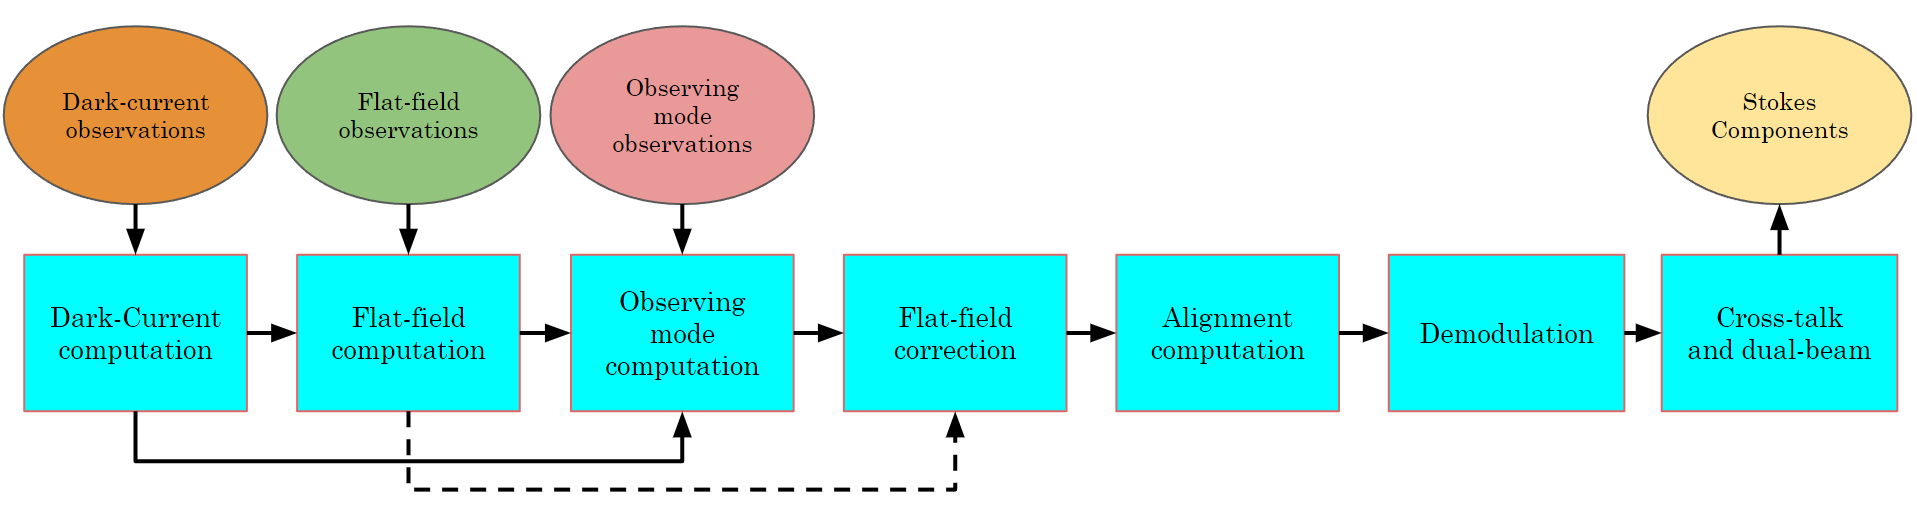
\includegraphics[width=\textwidth]{figures/Pipeline/pipeline_diagram.PNG}
  \caption{
    Block diagram of the standard reduction process: Blue boxes represent the individual steps that make up the reduction, while ellipses indicate the different sets of observations and the final product (yellow ellipse). }
    \label{fig_pipeline: block_diagram}
\end{figure}

The data reduction process begins with the dark-current processing, which involves averaging all individual dark frames within a specific set to generate a single dark-current frame per camera. This dark current is then subtracted from all images used in the reduction, including flat-fields, pinholes, and scientific observations, after rescaling the dark-current to the appropriate number of accumulations.

The second step is the flat-field computation. These observations, as previously mentioned, are a modified version of the nominal mode with an increased $\lambda_{\text{rep}}$ and are repeated $N_{\text{rep}}$ times. The processing involves averaging all images taken at a specific wavelength for the same modulation. Thus, $\lambda_{\text{rep}} \times N_{\text{rep}}$ images are averaged to produce a single flat-field frame. To maintain spectral line information, flat-fields are normalized to their mean value, as flat-fields taken at the line core have lower intensity than those in the continuum. The goal is to correct intensity variations within a single frame without altering relative intensities across different spectral points.

Having computed the dark-current and the flat-fields, the scientific observations can be corrected by substracting the dark-current and dividing the resulting image by the flat-field of the corresponding wavelength and modulation. 

\begin{figure}[t]
  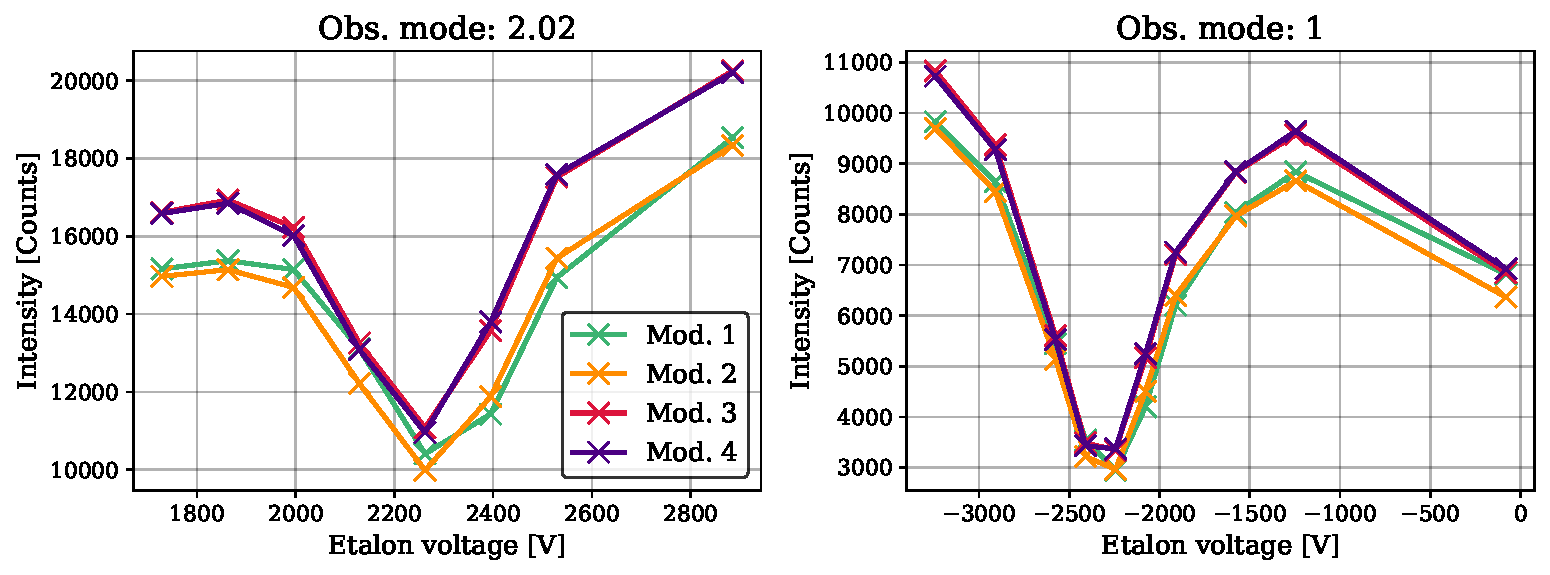
\includegraphics[width=\textwidth]{figures/Pipeline/Spectral_scans_ecample.pdf}
  \caption{
    Block diagram of the standard reduction process: Blue boxes represent the individual steps that make up the reduction, while ellipses indicate the different sets of observations and the final product (yellow ellipse). }
    \label{fig_pipeline: spectral_scans}
\end{figure}

After flat-fielding and dark current correction, the different modulations and the two cameras are combined to infer the stokes components for every measured wavelength. However, in order to combine the data from different cameras and modulations, the images have to be aligned beforehand. The alignment is carried out with the already corrected images and consists on a sequential process where the four modulations of the camera one are first aligned, and then the images of the second camera are aligned with respect to the image of the camera one and the corresponding modulation. The alignment is performed at subpixel accuraccy employing the methosd described in \cite{alignment}, where the alignement is computed employing a two-dimensional cross-correlation in the fourier domain. 

After alignment, the stokes components are derived through a process known as demodulation. This process is carried independently at different wavelengths and consists on a matrix multiplication employing the demodulation matrix and the four modulations in the vectroial scheme:
\begin{equation}
  \begin{pmatrix}
  I \\
  Q \\
  U \\
  V
  \end{pmatrix} = 
  \underbrace{\begin{pmatrix} 
      d _ {00} & d _ {01} & d _ {02} & d _ {03} \\ 
      d _ {10} & d _ {11} & d _ {12} & d _ {13} \\
      d _ {20} & d _ {21} & d _ {22} & d _ {23} \\
      d _ {30} & d _ {31} & d _ {32} & d _ {33} 
  \end{pmatrix}}_ {\textbf{D}}
  \begin{pmatrix}
    I _ {1} \\
    I _ {2} \\
    I _ {3} \\
    I _ {4}
    \end{pmatrix} \ \ , 
    \label{pipeline: Demod}
\end{equation}
where the matrix D is the inverse of the modulation matrix of the corresponding camera and pre-filter that were computed during the calibrations (see sec. \ref{sect:tumag_cal polarimetric}). And for the longitudinal scheme:
\begin{equation}
  \begin{pmatrix}
  I + V\\
  I - V
  \end{pmatrix} = 
  \begin{pmatrix} 
      d _ {00} & d _ {01} \\ 
      d _ {10} & d _ {11}
  \end{pmatrix}
  \begin{pmatrix}
    I _ {1} \\
    I _ {2} 
  \end{pmatrix} \ .
    \label{pipeline: Demod_long}
\end{equation}

From the matrix multiplication the stokes components for each camera are derived. However, the demodulation is never perfect, due to small deviations of the demodulation matrix from the real one, or instrumental artifacts that have been uncorrected by the flat-fielding. These defects result in a contaminated stokes components, where information from one component appears in other components, typically from Stokes I into Q, U, and or V. Nonetheless, these contamination, known as cross-talk, can be extracted from the data. 

The cross-talk correction is a manual process as different data sets require different corrections. For instance, some data sets may not show contamination from I to U while others do. Moreover, the correction might require to be applied using the information from the whole FoV or only of a small region. Thus, this is a correction that has to be carefully applied and its hard to standarize to the whole set of observations. Nonetheless, the concept of the correction is the same. 

The correction of the cross-talk from I to any other component starts by measuring the relation between the two components by fitting through a least-squares method, a polynomial of first order in order to compute the tendency, if there is one. Once this relation has been stablished, and the strength of the cross-talk (\textit{i.e.} the value of the slope) measured, the correction is applied by simply, removing the tendency of the data: 

\begin{equation}
  S_{corr} = S_{orig} - (I_{orig} * a + b),
\end{equation}
where the relation between the stokes component $S_{orig}$ and stokes I $I_{orig}$ has been fitted to the line: $S_{orig} =  I_{orig} * a + b$

\subsection{Extra calibration blocks.}

\subsection{Image reconstruction.}
\subsubsection{Linear polarizer calibration.}
\subsubsection{Micropolarizerss calibration.}
\subsubsection{Prefilter scans.}



% Challenges in data reduction
\chapter{\label{CH:challenges}Challenges in data reduction. Etalon Cavity Map.}

INTRO.
https://link.springer.com/article/10.1007/s10509-023-04212-3

\section{One device, two configurations.}

We established in section \ref{susec_spectropolarimeters: Imaging} that the observed intensity distribution at the coordinates $\xi$, $\eta$ of the focal plane of any etalon-based instrument tuned to a wavelength $\lambda_s$ obeys the following expression \citep{franI}: 

\begin{equation}
    I\left(\xi, \eta ; \lambda_{s}\right)=g(\xi, \eta)\int_{0}^{\infty} T(\lambda) \iint  O\left(\xi_0, \eta_0 ; \lambda\right)  \mathcal{S}\left(\xi_0, \eta_0; \xi , \eta; \lambda-\lambda_{s}\right)  \mathrm{d} \xi_{0} \mathrm{~d} \eta_{0}\mathrm{d} \lambda ,
    \label{eq_etalon_theory: General_Intensity}
\end{equation}
where $T(\lambda)$ accounts for the presence of an order-sorting pre-filter, $O\left(\xi_0, \eta_0 ; \lambda\right)$ represents the brightness distribution of the observed object at the point $\left(\xi_0, \eta_0\right)$, $S\left(\xi_0, \eta_0; \xi , \eta; \lambda-\lambda_{s}\right)$ accounts for the imaging response of the instrument when tuned at the wavelength $\lambda_{s}$, and $g(\xi, \eta)$ represents a spatial gain factor that accounts for wavelength independent pixel-to-pixel intensity fluctuations ocurring in the focal plane due to differences in the detectors' sensitivity. 

The imaging response of the instrument coincides with the PSF of the instrument when the optical response is invariant against translations. In such a case, we can substitute the last two integrals by the convolution operator, but this is not strictly true in etalon-based instruments, where the response varies pixel to pixel either because of etalon irregularities or because of variations in the illumination across its clear aperture.

Deriving S typically requires determining the electric field of the polychromatic wave in the image plane. According to \cite{franI}, this field can be calculated by summing all the electric fields $(E^{(t)})$ across the pupil, such that the eletric field at any point $(\xi, \eta)$ of the image plane follows the expression:

\begin{equation}
  E_{im} ^{(t)}(\xi, \eta) = \frac{1}{\pi R_{pup} ^2} \int \int _ {pupil} E^{(t)}(x, y)e ^{-ik( \xi x / f + \eta y / f)dx dy},
  \label{eq_etalon_theory: electric_image_plane}
\end{equation}
where $(x, y)$ are the coordinates in the pupil, $f$ stands for the focal length, and $R_{pup}$ is the radius of the pupil.  It can also be shown that the vector electric fields transmitted by the etalon can be expressed as:

\begin{equation}
  E ^{(t)}(\xi, \eta) = \frac{\sqrt{\tau}}{1 - R}\frac{e ^{i\delta / 2} - R e ^{ -i\delta / 2}}{1 + F \sin ^2 (\delta / 2)}E ^{(i)},
  \label{eq_etalon_theory: electric_transmitted}
\end{equation}
where $\tau$ is the transmission factor for normal incidence, $R$ stands for the reflectivity of the etalon mirrors, $F$ is a factor defined as $F \equiv 4R (1 - R )^{-2}$, $E^{(i)}$ are the incident electric fields, and $\delta$ stands for the phase differences between the transmitted and incident rays. 

The transmission profile of the etalon ($S$) is defined as the average ratio between the transmitted and incident intensities, calculated from the complex conjugate of the corresponding electric fields. The shape of $\delta$ varies depending on the illumination setup of the etalon, whether collimated or telecentric. Consequently, each configuration has unique solutions and characteristics and is differently affected by inhomogeneities (defects) in the etalon's properties.

\subsection{\label{susec_etalon_theory: collimated}Collimated configuration}

\begin{figure}
  \centering
  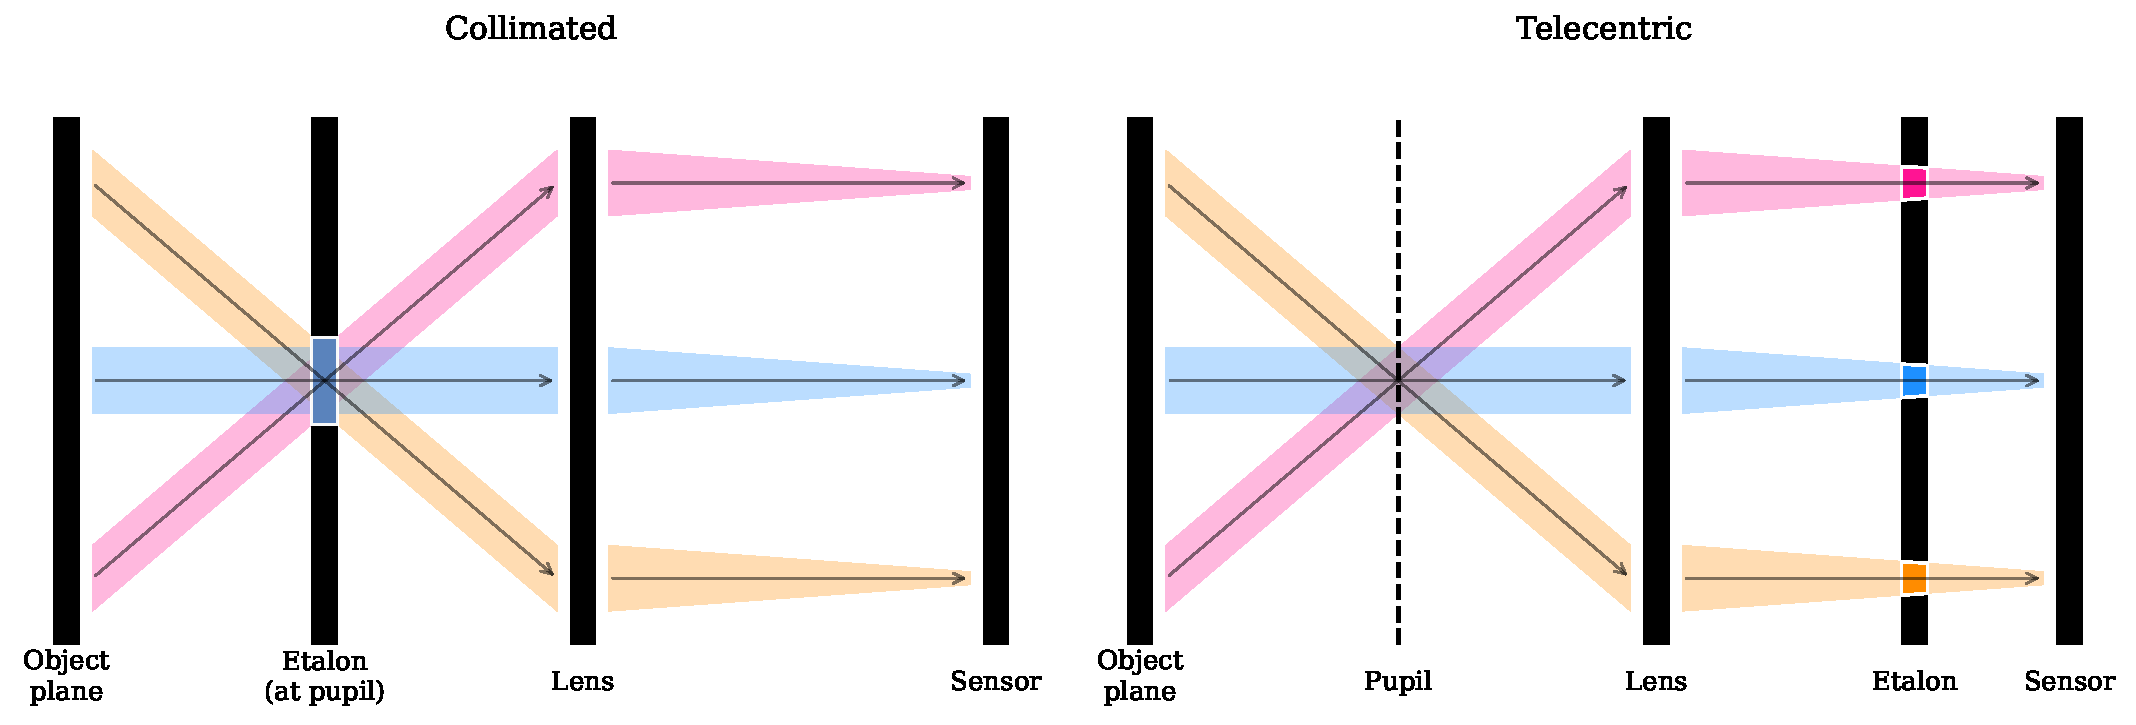
\includegraphics[width = \textwidth]{figures/EtalonChallenges/EtalonConfigurations.pdf}
  \caption{Schematic representation of the two optical setups of an FPI, collimated (left) and telecentric (right). The different colors represent distinct light rays originating from various points on the object plane. The white boxes in the etalon highlight the sections that are traversed by the light rays.
  } \label{fig_etalon_theory: Etalon configurations}
\end{figure}

Collimated mounts are characterized by having the etalon located at the pupil plane and therefore receive a collimated beam from each point of the observed object. As illustrated in the schematic on the left side of fig.~{\ref{fig_etalon_theory: Etalon configurations}}, light from any point on the object will fall on the same area of the etalon. Consequently, any local defects on the etalon crystals or on the plates' parallelism is averaged all over the clear aperture, thus making the optical quality constant along the FoV. However, the angle of incidence of the light beam varies along the FoV, thus shifting the spectral transmission profile.  

Analytical solutions of equation \eqref{eq_etalon_theory: electric_image_plane} are imposible to obtain if $\delta$ has a dependence on the pupil coordinates, as is the case of collimated etalons with a presence of local defects. In that case, the transmssion profile of the etalon has to be evaluated numerically. 

However, in order to study the spectral behavior of the transmission profile, we can, as a first-order approximation, disregard the spatial PSF and focus solely on the spectral transmission profile $(\psi)$. Under this assumption, the phase difference between the incident and transmitted rays of an ideal collimated etalon can be expressed as:  

\begin{equation}
  \delta (\xi, \eta, \lambda) = \frac{4\pi}{\lambda}nd\cos (\theta(\xi, \eta)),
  \label{eq_etalon_theory: collimated_delta}
\end{equation}
where $n$ stands for the refractive indx of the etalon cavity, $d$ is the distance between the mirrors and $\theta$ is the angle of incidence. In such a case, it can be shown that the spectral transmission profile follows the expression: 

\begin{equation}
  \psi\left(\xi, \eta, \lambda \right) = \frac{\tau}{1 + F \sin ^2 (\delta(\xi, \eta, \lambda) / 2)}.
  \label{eq_eta_theory : Collimated_profile}
\end{equation}

The spectral behaviour of the transmission profile, such as the spectral position of the resonance peaks and the distance between them (the free spectral range), is encoded in the parameter $\delta$, which is a function of the refractive index of the etalon cavity, the distance between mirrors, and the angle of the incident beam. The reflectivity $R$ of the mirrors determines the width of the resonance peaks through the parameter $F$, $F \equiv 4R (1 - R )^{-2}$.

Local defects in the collimated configuration are averaged out, which means that $d$ and $n$ respectively represent the mean values of the thickness and refractive index across the clear aperture of the FPI, and thus remain constant for every pixel. Yet, they produce a broadening of the transmission profile and worsen the optical quality of the instrument. However, the spatial dependence of $\psi$ naturally arises from $\theta$, which vcaries from pixel to pixel. 

Assessing the spatial PSF of the FPI is more challenging, as it can only be determined analytically for monochromatic light and in the absence of defects. We will not delve into the equations for this specific scenario as it lies beyond the scope of this thesis. However, interested readers are referred to the work of \cite{franI}, where this topic is extensively discussed.

\subsection{\label{susec_etalon_theory: Tele-perfe}Telecentric configuration}

In the telecentric configuration, the etalon is placed very close to an intermediate focal plane, while the pupil is focused at infinity. As shown in the sketch on the right side of fig.~{\ref{fig_etalon_theory: Etalon configurations}}, in this setup, the etalon is illuminated by cones of rays that are parallel to each other, thus passing through different sections of the interferometer. Local inhomogeneities (defects or cavities) on the etalon produce differences in the transmission profile across the FoV, which are directly mapped into the image plane. This means that the optical response and the transmission profile shift locally on the image sensor. 

In telecentric configurations, $\delta$ always depends on the coordinates of the pupil, even in the absence of defects, since each point in the etaon sees a cone of rays coming from different parts of the pupil. Thus, as stated before, solutions to equation \eqref{eq_etalon_theory: electric_image_plane} are to be found numerically. Nonetheless, if we neglect the spatial PSF once again, we can derive an analytical expression for an ideal telecentric etalon, where all light cones impact perpendicularly.

After some messy algebra and clever variable changes, one can recast eq. \eqref{eq_etalon_theory: electric_image_plane} in terms of the radial coordinates of the pupil and anallytically solve the equations. The resulting spectral transmission profile of an ideal telecentric etalon  is given by \citep{franIV}:
\begin{equation}
\Psi \left(\xi, \eta, \lambda \right) =  \mathfrak{Re}\left[E(a\left(\xi, \eta, \lambda \right), b\left(\xi, \eta, \lambda \right)) \right] ^2 + \mathfrak{Im}\left[E(a\left(\xi, \eta, \lambda \right), b\left(\xi, \eta, \lambda \right)) \right] ^2 ,
\label{eq_etalon_theory: Tel_first}
\end{equation}
with $E(a\left(\xi, \eta, \lambda \right), b\left(\xi, \eta \right))$ being:
\begin{multline}
E(a\left(\xi, \eta, \lambda \right), b\left(\xi, \eta \right)) = 2\sqrt{\tau}\Biggl\{ \frac{1}{\alpha_1}\left[\arctan(\gamma _ 1) - \arctan(\gamma_2)\right] + \\
\mathrm{i} \frac{1+R}{1-R} \frac{1}{\alpha_2}\left[\ln \left(\frac{(1 + \gamma _ 3) ^2 + \gamma _ 4 ^2}{(1 - \gamma _ 3) ^2 + \gamma _ 4 ^2} \right) - \ln \left(\frac{(1 + \gamma_ 3) ^2 + \gamma _ 5 ^ 2}{(1 - \gamma _ 3) ^2 + \gamma _ 5 ^2} \right)\right]\Biggr\},  
\end{multline}
where, the auxiliary functions are defined as:
\begin{equation}
\begin{split}
a\left(\xi, \eta, \lambda \right) &\equiv \frac{2 \pi}{\lambda}n\left(\xi, \eta\right)d\left(\xi, \eta\right) \ , \\
b\left(\xi, \eta\right) &\equiv \frac{1}{8n\left(\xi, \eta\right)^2(f\#) ^2}\ ,  \\
\alpha _ 1 &\equiv 2ab\sqrt{F}\ ,  \\
\alpha _ 2 &\equiv 2\alpha_ 1\sqrt{F + 1}\ ,  \\
\gamma _ 1 &\equiv \sqrt{F} \sin a\ ,  \\
\gamma _ 2 &\equiv \sqrt{F} \sin (a[1 - b])\ ,  \\
\gamma _ 3 &\equiv \sqrt{\frac{F}{F + 1}} \ ,  \\
\gamma _ 4 &\equiv \frac{\tan \left( a/2 [1 - b] \right)}{\sqrt{F + 1}}\ ,  \\
\gamma _ 5 &\equiv \frac{\tan (a/2)}{\sqrt{F + 1}}\ .
\end{split}
\end{equation}

The parameter $a$ has the same role as $\delta$ for the collimated case. However, the dependence on the image plane coordinates in this case is caused by potential variations in n and/or d, as each light beam traverses different sections of the etalon. These variations constitute the "cavity map" of a telecentric etalon and must always be taken into account during data reduction processes.

The parameter $b$ accounts for the contribution of the focal ratio, $f\#$, and has an impact on the spectral resolution and the apodization of the pupil as seen from the etalon \citep{beckers}. Thus, the resolution is now affected by both $F$ and $f\#$, through the parameters $a$ and $b$.

\subsubsection{\label{etalon_theory: Tele-imperfe}Telecentric imperfect configuration}
The equations shown in Sect.~\ref{susec_etalon_theory: Tele-perfe} are valid whenever the incident cone of rays is perpendicular to the etalon mirrors. We refer to this situation hereinafter as "perfect telecentrism". However, real instruments are likely to present deviations from such an ideal case. These deviations can be caused by an intentional tilt of the etalon to suppress ghost images on the detector \citep{ghosts-etalon}, by an accidental tilted angle of incidence caused by deviations from the ideal paraxial propagation of rays within the instrument, or simply because of misalignment of the optical components. In the three cases, the incident cone of rays is no longer perpendicular to the etalon, and hence, we consider these scenarios to have imperfections in the telecentrism degree. One important consequence of the loss of telecentrism is an asymmetrization of the transmission profile that must be accounted for when modeling the instrument response.

The transmission profile in this case is influenced by the angle of incidence of the chief ray at each point of the clear aperture of the etalon, in addition to the parameters mentioned in the previous sections. Unfortunately, the equations for the transmission profile in these configurations are much more complicated than in the ideal case, and can no longer be anallytically solved. We must revisit equation \eqref{eq_etalon_theory: electric_image_plane} and solve the integrals numerically.

\begin{figure}
    \centering
    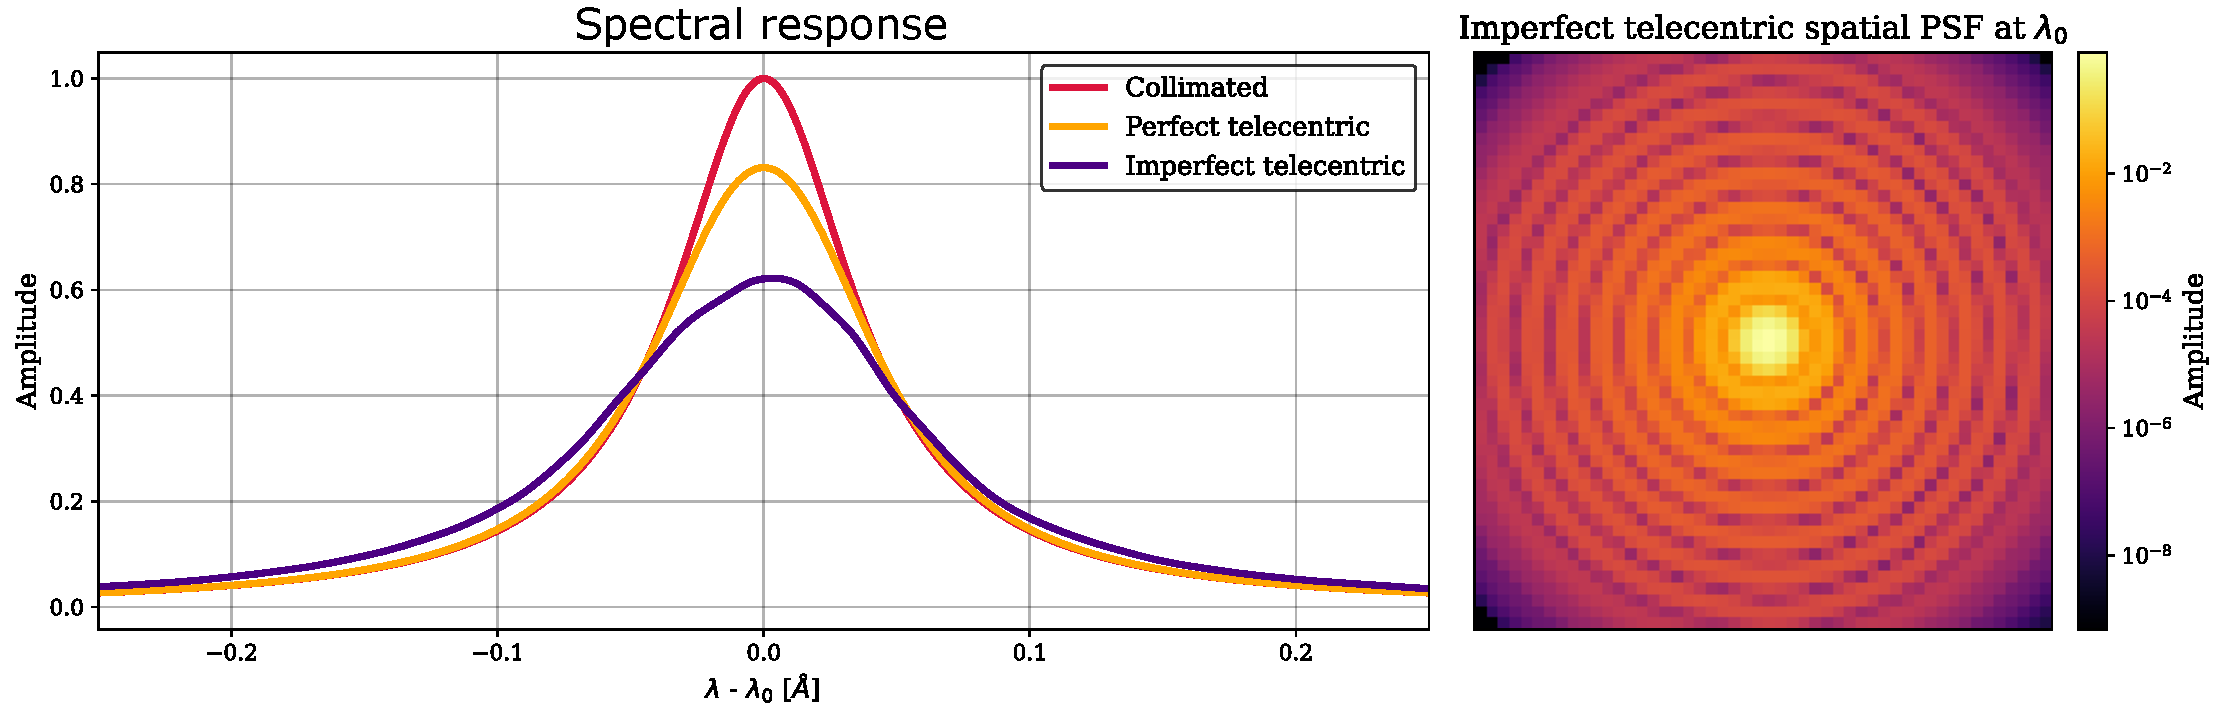
\includegraphics[width = \textwidth]{figures/EtalonChallenges/etalon_setups_profiles.pdf}
    \caption{\textit{Left}: central peak of the etalon's spectral transmission profile for the three different configurations. \textit{Right}: Spatial PSF of the imperfect telecentric etalon at $\lambda _ 0$. The parameters of the etalon are $R = 0.92$, $n = 2.29$, $d = 251 \, \mu \mathrm{m}$, $f\#=56$, $\theta = 0 ^{\circ}$ (collimated and perfect telecentric), and $\Theta = 0.3\,^{\circ}$ (imperfect telecentric).}
    \label{fig_etalon_theory:Profiles-configs}
\end{figure}

Figure \ref{fig_etalon_theory:Profiles-configs} shows on the left the transmission profile corresponding to the three different scenarios: collimated illumination of the etalon, perfect telecentrism, and imperfect telecentrism. The etalon parameters have been selected to coincide with those of SO/PHI's etalon. In both the collimated and perfect telecentric configurations, a normal incidence  ($\theta = 0$) scenario is shown, whereas in the imperfect telecentric case, we assumed an angle of incidence of the chief ray, $\Theta$, of $0.3^{\circ}$. The parameter $a$ has been adjusted slightly in order to tune the transmission profile at $\lambda _ 0$. 

Regarding the properties of each profile, note that the telecentric configurations achieve lower peak transmissions than the collimated case. In addition, the telecentric profiles are wider due to the different incidence angles across the illuminating cone of rays. Such a broadening increases with decreasing f-ratios. Lastly, non-normal incidence of the chief ray in the telecentric configuration further widens and shifts ($\sim 4$~m\r{A}
for $\Theta=0.3^\circ$) the profile, making it asymmetrical. 

\section{Sunspot observation simulation}
INTRO sunspot. Challenges in data reduction, unknown effects etc. 

\subsection{Simulated data.}

blabla
\subsection{Observations simulation.}

All the instruments built around the use of an etalon as a wavelength filtering element operate in a very similar way. They scan a spectral line by tuning the etalon (by changing the distance between mirrors and/or modifying the refractive index) to a desired number of wavelengths along the spectral line. At each spectral position, the solar scene is recorded. The measured intensity is approximately given by Eq.~\eqref{eq_etalon_theory: General_Intensity}, with the etalon's transmission profile centered at the desired wavelength.

We have carried out two sets of simulations, one with a perfect telecentric configuration, where the incidence is normal, and one with an angle of incidence of the chief ray is $0.5^\circ$. For each of these sets, a simulated observation of the sunspot has been carried out employing 45 wavelengths for the scan of the line. A flat-field observation has also been computed with the same configuration than the one employed for the suspot observation. For the flat-field observations we have generated an \textit{ideal} flat-field where the average profile computed in quiet-sun was replicated at every pixel of the generated image.

\begin{figure}
    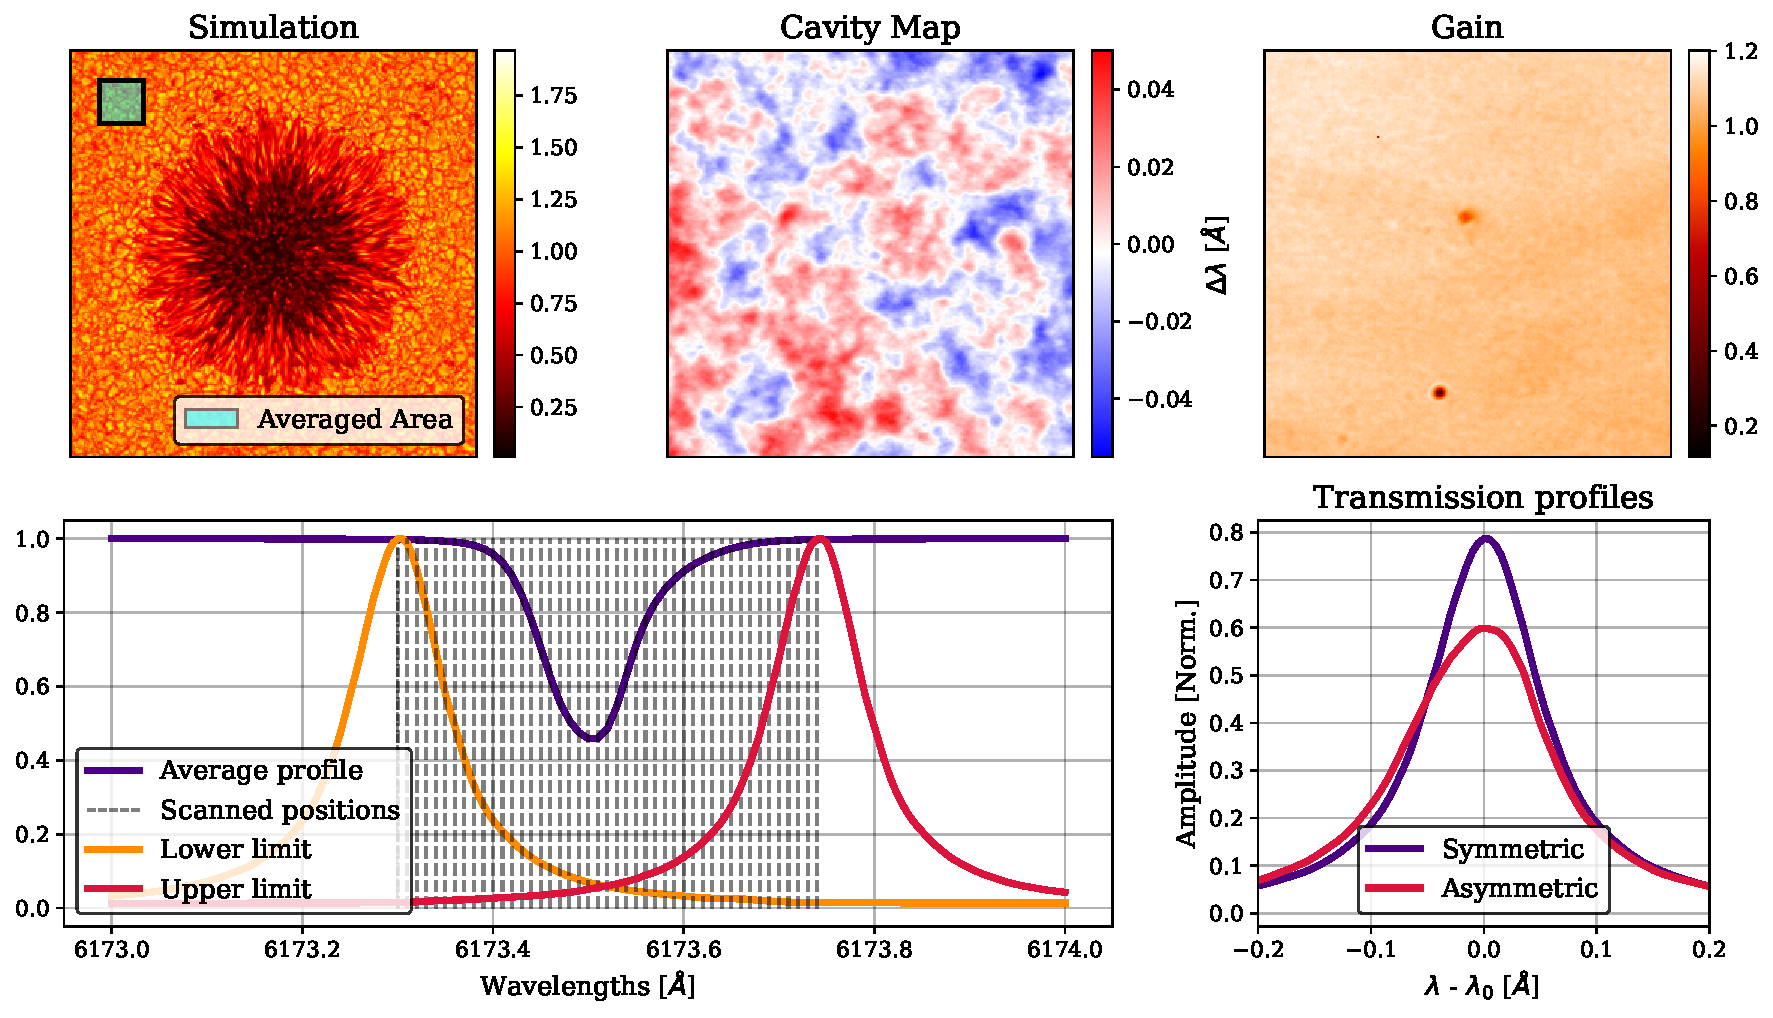
\includegraphics[width=\textwidth]{figures/Mancha/Inputs_mancha.pdf}
    \caption{
      Inputs for the simulation of the sunspot observation. The top row shows, from left to right, the continuum of the MHD simulation, the cavity map expressed as the corresponding shift in \r{A} and the gain map. The bottom row shows, again from left to right, a representation of the quiet-sun average profile with all the scanned wavelengths, and the transmission profile of the two different FPI configurations, the symmetric (perfect telecentric) and asymmetric (imperfect telecentric). The parametets employed for the etalon are: XXXXX.
      \label{fig_mancha: Inputs}}
\end{figure}

Although, in practice, it is not often possible to fully characterize the pre-filter, we assumed it has a rectangular shape centered at the wavelength of the observed spectral line ($\lambda _ {0}$) and a width of $2\Delta \lambda$ such that only one order of the etalon passes through. With this consideration, equation \eqref{eq_eta_corr: intensity} can be written as follows:

\begin{equation}
  I\left(\xi, \eta ; \lambda_{s}\right)=g(\xi, \eta)\int_{\lambda _ 0 - \Delta \lambda}^{\lambda _ 0 - \Delta \lambda} \iint  O\left(\xi_0, \eta_0 ; \lambda\right)  \mathcal{S}\left(\xi_0, \eta_0; \xi , \eta; \lambda-\lambda_{s}\right)  \mathrm{d} \xi_{0} \mathrm{~d} \eta_{0}\mathrm{d} \lambda \ .
  \label{eq_mancha: Intensity}
\end{equation}

For every tuned wavelength, the instensity in a given pixel is given by equation \eqref{eq_mancha: Intensity}, where the observed object is the sunspot simulation or the generated \textit{ideal} flat-field. 

The imaging response of the FPI is computed by solving the integrals in equation \eqref{eq_etalon_theory: electric_image_plane}. Given that we will account for the PSF in these simulations, numerical methods are necessary to evaluate the integrals. The computational burden is significant, as the integrals must be evaluated $N_{pixel} ^2 N_{\lambda} N_{mods} N_{sets} > 10 ^8$ times\footnote{$N_{pixels} = 561$, $N_{\lambda} = 45$, $N_{mods} = 2$, $N_{sets} = 2$} for both sunspot and flat field observations. This extensive computation results in excessively long simulation times. To address this issue, a neural network was developed to reduce the computational time from \textcolor{red}{X to X}. The neural network was trained with known solutions to the integrals for a fixed set of etalon parameters, ensuring that its outputs are accurate to within 0.01\% for parameters within the training set.

In real-world scenarios, variations in pixel sensitivities (gain) and etalon imperfections (cavity map) are unavoidable. Including the effect of the gain into the simulation is straigghtforward as it only acts as a multiplicative factor that modifies the final intensity. In contrast, the effects of the cavity map are more cumbersome. Pixel-to-pixel variations in etalon defects shift the transmission profile of the Fabry-Perot Interferometer (FPI) and must be accounted for when computing the imaging response. Both the gain and cavity map introduced in the simulations have been selected to resemble the real-case scenario of the SO/PHI instrument. The gain map (Figure XXX a) utilized in the simulations is derived from a flat field of the High Resolution Telescope (HRT) instrument, while the cavity map employed (Figure XXX a) is sourced from the cavity map of PHI's etalon.


\section{Fitting algorithm}
\subsection{\label{eta_corr_susec: etalon_transmission}Initial approximations}

As an initial approximation, we will disregard the spatial PSF and assume that the spatial dependence can be represented by a Dirac delta function to simplify the equations. Therefore, if we assume that the image response of the FPI follows the expression:
\begin{equation}
S\left(\xi_0, \eta_0; \xi , \eta; \lambda-\lambda_{s}\right)=\delta(\xi_0-\xi,\eta_0-\eta)\Psi(\xi,\eta,\lambda-\lambda_s),
\end{equation}
equation \eqref{eq_etalon_theory: General_Intensity} simplifies into:
\begin{equation}
    I\left(\xi, \eta ; \lambda_{s}\right)=g(\xi, \eta)\int_{0}^{\infty} T(\lambda)  O\left(\xi, \eta ; \lambda\right) \Psi\left(\xi, \eta ; \lambda-\lambda_{s}\right)  \mathrm{d} \lambda.
    \label{eq_eta_corr: intensity}
\end{equation}



The explicit shape of $\Psi$ is different depending on the optical configuration of the instrument, that is, collimated or telecentric.

\subsection{\label{eta_corr_susec: simulating obs} Simulated observations}
  
  
We carried out a series of simulations of a spectral line observation in different conditions. We used the Kitt Peak FTS-Spectral-Atlas as the reference \citep{fts} and, specifically, the Fe I spectral line at 6173.3~\r{A}. Each observation was composed of $N_\lambda$ wavelengths, where the measured intensity was recorded. At every wavelength $\lambda_s$, the corresponding transmission profile of the etalon $\Psi^{\lambda_s}$ was computed, and the "observed" intensity $I ^{\lambda _ s} _ {{\rm obs}, i}$ corresponding to a specific spatial location $(\xi, \eta)$, represented hereinafter by the pixel $i$, was calculated using Eq.~\eqref{eq_eta_corr: Intensity-final}. Additionally, we took into account the presence of additive Gaussian noise. This noise does not necessarily respond to any parameter fluctuation within our analytical expressions or photon noise but comes from any unexpected variations that may not have been modeled in the theoretical scheme.

Additionally, we included the presence of defects arising from irregularities or inhomogeneities on either the cavity thickness $d$, the refractive index $n$, or from deviations of the angle of incidence $\theta$. In order to simulate this, we introduced a relative perturbation $\Delta a$ into the etalon equation that accounts for any local deviation of the value of $a$ with respect to its nominal value. This parameter changes from pixel to pixel differently for the collimated and telecentric configurations. In the former, the profile shifts across the FoV only because of the different incidence angles of the light beam on the etalon. In the latter, local variations of $n$ and/or $d$ are mapped directly onto the detector. We also note that variations in the incidence angle must be considered as well when the degree of telecentrism varies along the detector. Analytically, the parameter $a$ at each $i$-th pixel is given by $a' _ i = a \Delta a _ i$, where $a = (2\pi/\lambda) n d\cos\theta$ is constant along the FoV. Note that rewriting the equations for the transmission profiles (sections \ref{susec_etalon_theory: collimated} and \ref{susec_etalon_theory: Tele-perfe}) using this definition of $a$ is straightforward. In collimated configurations, the parameter $\delta$ (eq. \eqref{eq_etalon_theory: collimated_delta}) is simply $2a$. In perfect telecentric configurations, $\theta$ is always 0, so the given transmission profile is already expressed in terms of $a$.   

We let $n _ i ^{\lambda_s}$ be the  noise contribution at the $i$-th pixel and wavelength $\lambda_s$. Thus, the observed intensity at that pixel when the etalon is tuned at $\lambda _s$, $I ^{\lambda _ s} _ {{\rm obs}, i}$ is given by 
\begin{equation}
I ^{\lambda _ s} _ {{\rm obs}, i} = g_i \frac{\int_{\lambda_0 - \Delta \lambda}^{\lambda_0 + \Delta \lambda} O(\lambda)\Psi^{\lambda _ s} (\lambda , \Delta a _i)  d\lambda}{\int_{\lambda_0 - \Delta \lambda}^{\lambda_0 + \Delta \lambda} O(\lambda)\Psi^{\lambda _ c} (\lambda, \Delta a _ i)  d\lambda} + n _ i ^{\lambda_s}    ,
\label{eq_eta_corr: Profile - General}
\end{equation}
with $\lambda _ c$ being the continuum wavelength. From a practical point of view, the integration limits are set in such a way that only a single resonance (or order) of the etalon is included with the limits, thus, acting akin to the sorting pre-filter commented on previously. We note that the denominator strictly corresponds to the intensity at the continuum of the line in the absence of the transmission profile or if the continuum wavelength is far enough from the spectral line. In any other case, the transmission should be taken into account as well to normalize the observations to the local continuum, which is necessary since we work with relative measurements. An example of a spectral line measurement is displayed in Fig.~\ref{fig_etalon_corr: Prof-Measure}.
\begin{figure}
    \centering
    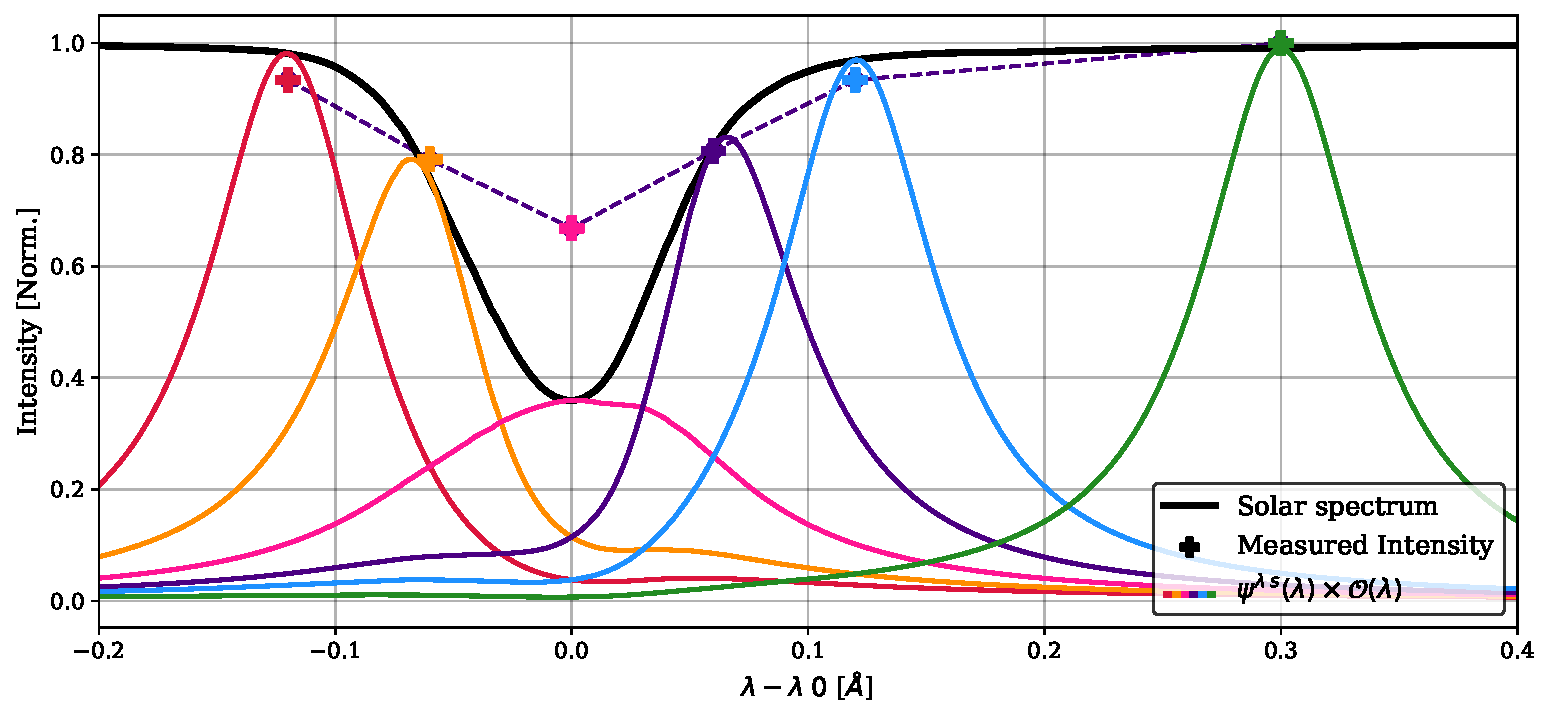
\includegraphics[width = \textwidth]{figures/EtalonPaper/ProfileMeasurement.pdf}
    \caption{Simulated observation of the Fe I spectral line ($\lambda _ 0 = 6173.3$\r{A}) using a collimated mount and a total of $N_ \lambda = 6$ wavelengths that have been equally distributed along the spectral line, with the exception of the continuum measurement (light blue), which is selected at $300$ m\r{A} from the blue of the line core. The measured intensity is the result of computing the value given by Eq.~\ref{eq_eta_corr: Profile - General} at each wavelength and with $g = 1$.
    } \label{fig_etalon_corr: Prof-Measure}
\end{figure}

For both the collimated and telecentric configurations, we modeled etalon and gain imperfections over a $100\times100$~px$^2$ image. Pixel-to-pixel variations in the sensor efficiency were modeled following a random spatial distribution, as shown in Fig.~ \ref{fig_etalon_corr: Inputs} (top panel). Additionally, we included a set of pixels with very low gain values, which represent a group of dead pixels or dust grains.

We modeled the etalon defects as changes in $\Delta a$ in such a way that the maximum displacement reaches $3$ pm. The spatial distribution of the values of  $\Delta a $ follows an increasing radial distribution, as shown in Fig.~ \ref{fig_etalon_corr: Inputs} (bottom panel). Such a spatial distribution coincides with the expected one in collimated etalons due to the change in the incidence angle across the FoV. Telecentric mounts do not exhibit a spatial distribution of their defects such as this, but using the same spatial distribution in the two cases allowed us to compare the performance of the method for both setups in a systematic way. Since $\Delta a$ accounts for relative perturbations, it is by definition an adimensional parameter. However, to grant it a physical meaning, we express the values of $\Delta a$ in \r{A}, representing the associated shift of the transmission profile with respect to the original position determined by $a$.

\begin{figure}
  \centering
    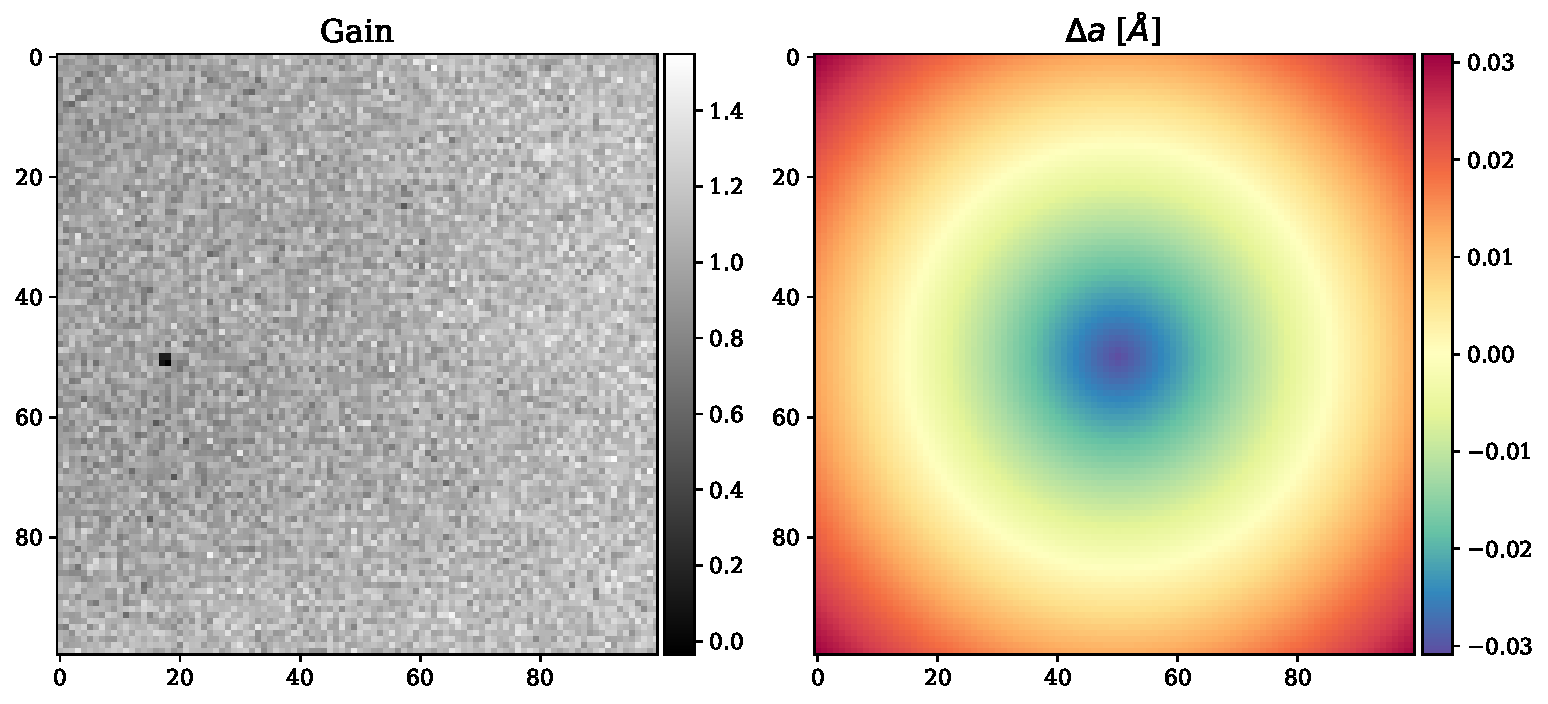
\includegraphics[width=\textwidth]{figures/EtalonPaper/Gain_Da_Inputs.pdf}
    \caption{
      Input maps introduced when simulating the observations. The left panel represents the gain generated as white Gaussian noise, with values ranging from 0.8 to 1.2. A dust speck was introduced by creating a group of four pixels with low values of $g=0.2$ for the gain. The right panel shows the spatial distribution of the defects in the etalon. The distribution follows a radial pattern starting from the center of the FoV. The defects vary from $0\,\%$ deviation to up to $5\times 10 ^{-4}\,\%$, which corresponds to a shift of 3~pm. Both possible directions for the deviations have been considered. The sign of the deviation is negative at the very center, which introduces a redshift, while it is positive at the corners, causing a shift of the profile into the blue.
      \label{fig_etalon_corr: Inputs}}
\end{figure}

\section{\label{eta_corr_susec: fitting algorithm}Fitting algorithm}

We have developed an algorithm able to extract the distribution of the etalon defects and the gain map from data taken by etalon-based instruments, which enables the correction of the two contributions separately. The algorithm works by minimizing a given merit function that depends on the gain and the etalon defects. 

In particular, we have defined an error metric, $\varepsilon  ^\lambda$, at each tuned wavelength, computed by comparing the measured intensity with the theoretical prediction. If we let $I_ {i, {\rm obs}} ^{\lambda _s}$ be the measured intensity at a given $i$ pixel for an etalon tuned to the wavelength $\lambda_s$, the error metric at each wavelength is given by
\begin{equation}
\varepsilon ^{\lambda _s} (\Delta a _i, g _ i) =  I _ {i, {\rm obs}} ^{\lambda _ s} - g_i \frac{\int_{\lambda_p}^{\lambda_q} O(\lambda)\Psi^{\lambda _ s} (\lambda, \Delta a _ i)  d\lambda}{\int_{\lambda_p}^{\lambda_q} O(\lambda)\Psi^{\lambda _ c} (\lambda, \Delta a _ i)  d\lambda}
\label{eq_eta_corr: Error metric}.
\end{equation}

The merit function we employed is then the quadratic summation of the error metric over all tuned wavelengths:

\begin{equation}
f(\Delta a _i, g _ i) = \sum _ {s = 0} ^ {N_\lambda} \left( \varepsilon ^{\lambda _s} (\Delta a _i, g _ i) \right) ^ 2.  
\label{eq_eta_corr: Merit Function}
\end{equation}
Both the camera gain and the defects of the etalon change from one pixel to another, which is why we address each pixel independently, but they remain constant at every wavelength. Hence, the transmission profile of the etalon varies at different points of the FoV; but at a given pixel, it is constant at all tuned wavelengths. Therefore, the algorithm is able to better obtain the etalon properties as we increase the number of wavelengths.

Figure \ref{fig_etalon_corr: Derivatives} shows the derivatives of the error metric, Eq.~\eqref{eq_eta_corr: Error metric}, as a function of wavelength, that is, before computing the summation over $s$ of the merit function, with respect to the gain, the reflectivity, and $\Delta $a. The curve corresponding to the $\Delta a$ derivative is different from the others, whereas the derivatives of both the gain and the reflectivity exhibit similar shapes. Hence, variations in either the reflectivity or the gain introduce similar changes in the merit function, which can produce a trade-off between these two parameters, especially when the spectral line is sampled in only a few points. Given that discrepancies arising from errors in reflectivity are assimilated by gain maps, we did not take into account reflectivity errors when computing our simulations, as they have no impact on cavity map calculations.

\begin{figure}
  \begin{minipage}[c]{0.6\textwidth}
    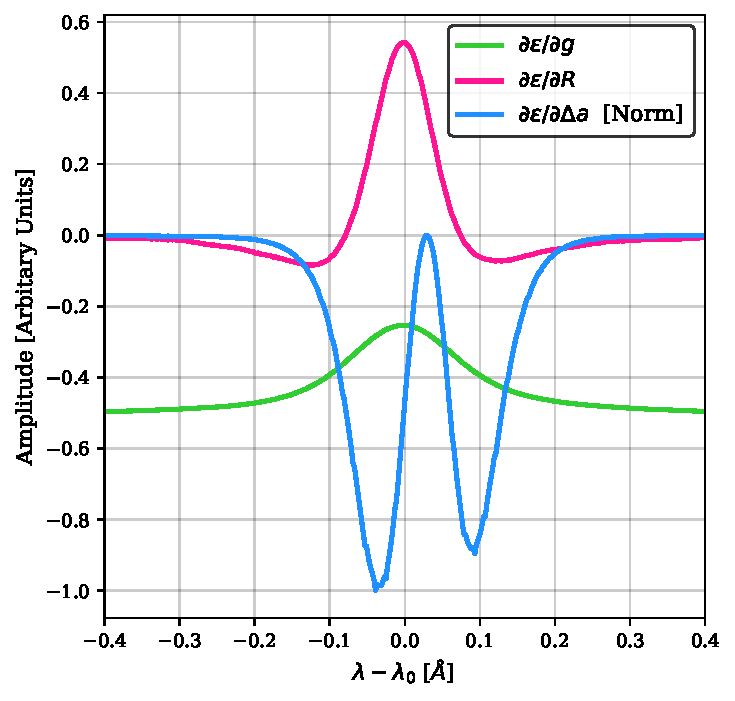
\includegraphics[width=\textwidth]{figures/EtalonPaper/Derivadas.pdf}
  \end{minipage}\hfill
  \begin{minipage}[c]{0.37\textwidth}
    \caption{
      Derivatives of the error metric as a function of wavelength. The derivative with respect to $\Delta a$ has been normalized in order to fit the three curves in the same plot. \label{fig_etalon_corr: Derivatives}} 
  \end{minipage}
\end{figure}


A few key aspects arise when analyzing the merit function and its applicability on real data. The first point to bear in mind is that the shape of the object, $O(\lambda)$, is not known a priory. Therefore, we needed to provide a guess for it. The method works by assuming that differences between the prediction and the observation are caused exclusively by the etalon defects or the gain. If the object used during the fitting process differs considerably from the real one, the prediction and observation will have differences that will erroneously be identified as etalon defects or gain variations. This is the main source of errors for the method when applied to real data. Two approaches can be followed in order to address this issue. The first one consists of assuming the solar atlas profile as the object. This is a good approximation, provided the data to which the algorithm is applied to lack information about solar structure, either because they are observations of long integration times of the quiet sun or produced by averaging several quiet sun observations (flat fields). If this condition cannot be met, this approach is not valid. The second approach involves deriving an approximated object from the data themselves by deconvolving the mean profile of the observation with the etalon's transmission profile. This approach can account for any difference the real object may have with the solar atlas and thus has a greater resemblance to the real object. Nevertheless, the process of deconvolving is prone to errors when the sampling is insufficient and can introduce additional noise into the problem. We have tested both approaches to compare their performances on different scenarios in order to assess when to use one or the other.

\begin{figure}
\centering
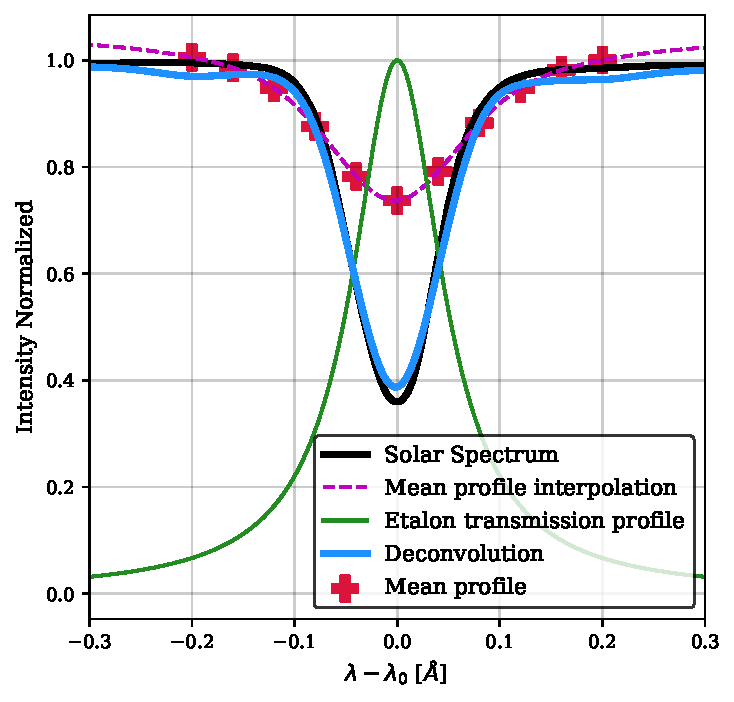
\includegraphics[width=\textwidth]{figures/EtalonPaper/Deconvolution.pdf}
\caption{Deconvolution of the object with a measurement of the Fe I spectral line using $N_\lambda = 9$. All points of the FoV have been used to compute the average profiles (blue crosses). The deconvolution (orange) is the result of deconvolving the mean profile interpolation (dashed line) with the displayed etalon transmission profile (red).\label{fig_etalon_corr:Deconvolution} }
\end{figure}

We employed Newton's method to minimize the merit function, Eq.~\eqref{eq_eta_corr: Merit Function}, as it has been proven to quickly converge (in five iterations or fewer, usually). The method begins by assuming an initial guess for the gain $g_j$ and $\Delta a_j$ parameters. Then, provided the initial guess is sufficiently close to the solution and that the merit function is continuous and differentiable, the gain $g_j$ and $\Delta a_j$ encoded in the vector, $\mathbf{x}_j$, can be updated iteratively at each iteration, $j$, as

\begin{equation}
\mathbf{x} _ {j + 1} = \mathbf{x} _ j - \mathcal{H} ^ {- 1} \mathcal{J} ^ T f(\mathbf{x}_j) \ , 
\end{equation}

where $\mathcal{H}$ and $\mathcal{J}$ are the Hessian and Jacobian matrices of the merit function $f$, respectively, calculated for $\mathbf{x}_j = [g_j,\Delta a_j]^T$, and $T$ stands for the transpose. Hence, the transmission profile of the etalon and its derivatives have to be computed for every wavelength and every pixel at each iteration. This can be computationally costly, especially when using imperfect telecentric configurations, where numerical integrals are involved. All derivatives needed for the algorithm are calculated analytically, except when simulating imperfect telecentrism. A detailed formulation of these derivatives is provided in the appendix.

Regarding the object $O(\lambda)$, if we assume it is given by the solar atlas, no additional computations are needed. However, when using the deconvolution approach, the object has to be calculated in each iteration. In this case, the algorithm works as follows: First, we compute the average profile across the whole FoV, and we force the continuum intensity to be the same on both sides of the spectral range to reduce the boundary effects of the deconvolution. This step is only necessary in case the spectral line is sampled in only a few positions, as is the case of the SO/PHI, IMaX, or TuMag instruments, where only a continuum point, either at the red or the blue side of the spectrum, is recorded. Both the object and transmission profile require a good spectral sampling to accurately compute the integrals of Eq.~\eqref{eq_eta_corr: Error metric}. Second, a cubic spline interpolation is applied to the generated average profile to artificially improve the spectral sampling, if necessary. Finally, the interpolated profile is then deconvolved by means of a Wiener filter with the etalon's transmission profile. The result of this deconvolution is the object, $O(\lambda)$, used in the minimization algorithm. The deconvolution of the object is done every time the etalon defects are updated in order to improve the resemblance of the deconvolved object to the real one. Figure \ref{fig_etalon_corr:Deconvolution} shows an example of this process in a simulated observation using nine scanned points and a collimated configuration. The deconvolution manages to reproduce the original signal, with only some minor differences in the line core and the beginning of the wings.

\subsection{\label{eta_corr_susec: results}Test scenarios and results}

The aim of the simulations carried out in this section was to characterize the role of the noise $\delta _ i ^ {\lambda_s}$, the spectral sampling, the selection of the object $O(\lambda)$, and the accuracy of the method for both the collimated and telecentric configurations. All simulations were run for different choices of the number of scanned wavelengths, ranging from $N_\lambda=5$ to $N_\lambda=21$. 

\subsubsection{Impact of the noise level}
We first assumed that the spectrum of the observed object is given by the solar atlas. This way, all errors in the derivation of the gain and etalon defects only come from the noise introduced into the measurement. We refer to this as the "ideal case." Since we were combining different measurements taken at different wavelengths, we considered a worst-case scenario and simulated three different signal-to-noise ratios: 100, 150, and 200. 

We restricted imperfections in the telecentrism to arise only for one scenario, S/N~$=200$, since simulating imperfections requires a high computational effort due to the lack of a theoretical expression for both the transmission profile and its derivatives. We also assumed that the degree of telecentrism ($0.3 ^\circ $) is known in this case.

\begin{figure}
    \centering
     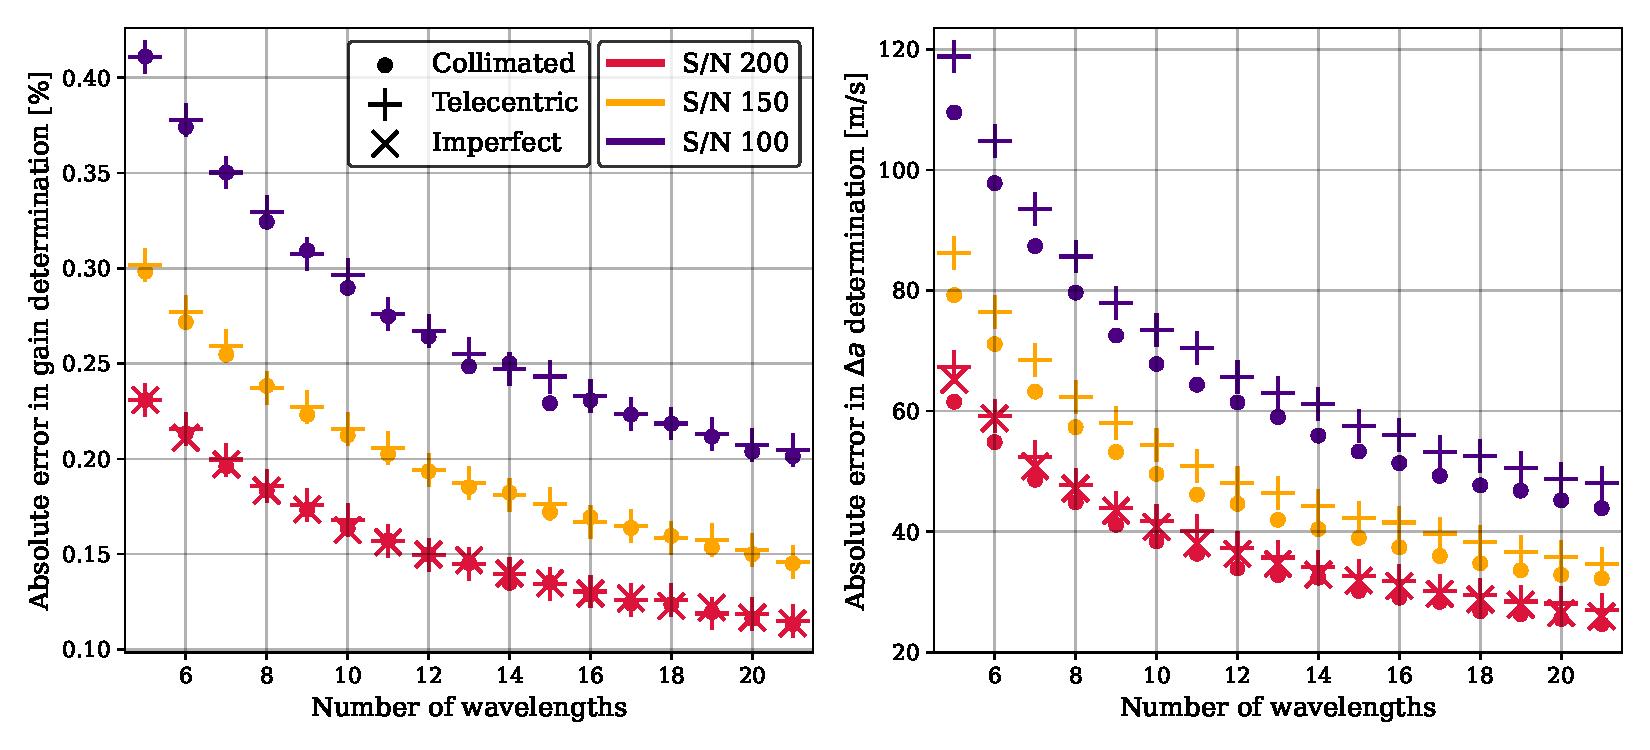
\includegraphics[width=\textwidth]{figures/EtalonPaper/SNR_plot_imperfect.pdf}
    \caption{Absolute errors of the gain (left) and etalon defect (right) derivations averaged over all the FoV. The number of wavelengths corresponds to the parameter $N_\lambda$ of wavelengths used to scan the profile.\label{fig_etalon_corr:SNR_both}}
\end{figure}

Figure \ref{fig_etalon_corr:SNR_both} shows the average absolute error in $g$ (left panel) and in $\Delta a$ (right panel) over the whole FoV as a function of the wavelength sampling, $N_\lambda$. The error in $g$ is expressed as a percentage of its real value. Errors in $\Delta a$ are given in meters per second since they are mostly responsible for shifting the profile. Errors in $\Delta a$ can be translated into velocity errors by computing the doppler velocity (Eq. \eqref{eq_spectro: Doppler}) associated to the spectral shift of the transmission ppeak produce by the error in $\Delta a$.
Figure \ref{fig_etalon_corr:SNR_both} shows the average absolute error in $g$ (left panel) and in $\Delta a$ (right panel) over the whole FoV as a function of the wavelength sampling, $N_\lambda$. The error in $g$ is expressed as a percentage of its real value. Errors in $\Delta a$ are given in meters per second since they are mostly responsible for shifting the profile. Errors in $\Delta a$ can be translated into velocity errors by computing the doppler velocity (Eq. \eqref{eq_spectro: Doppler}) associated to the spectral shift of the transmission ppeak produce by the error in $\Delta a$.

All the scenarios exhibit a similar behavior as far as their dependence on the spectral sampling is concerned, namely, the absolute errors decrease monotonically when the wavelength sampling increases. The reason for this is simply that a larger number of wavelength samples increases the amount of available information that the algorithm can use, thus making the fitting for $g$ and $\Delta a$ more precise. These results highlight the importance of properly sampling the targeted spectral line. A modest sampling of only $N_\lambda=5$ can produce errors as large as $120 \, {\rm ms^{-1}}$ in the worst-case scenario (S/N = 100). 

The noise level also plays an important role in the accuracy of the results. Scenarios with a lower S/N always have larger errors, for a given $N_\lambda$, in both the gain and $\Delta a $ computations. The difference in the performance of the algorithm due to the noise also changes with the spectral sampling; scenarios with a poor spectral sampling suffer from larger differences in the accuracy between the different S/N (50 ms$^{-1}$ for $N_\lambda$ = 5 between S/N = 200 and S/N = 100) than those with higher samplings (35 ms$^{-1}$ for $N_\lambda = 21$).

The optical configuration of the etalon has a very small impact on the accuracy of the algorithm. Results for the three setups are very similar, particularly in the gain calculation, for which the results are almost identical for all configurations. Retrieval of $\Delta a$ is slightly better for the collimated mount, though.

\begin{figure}
    \centering
    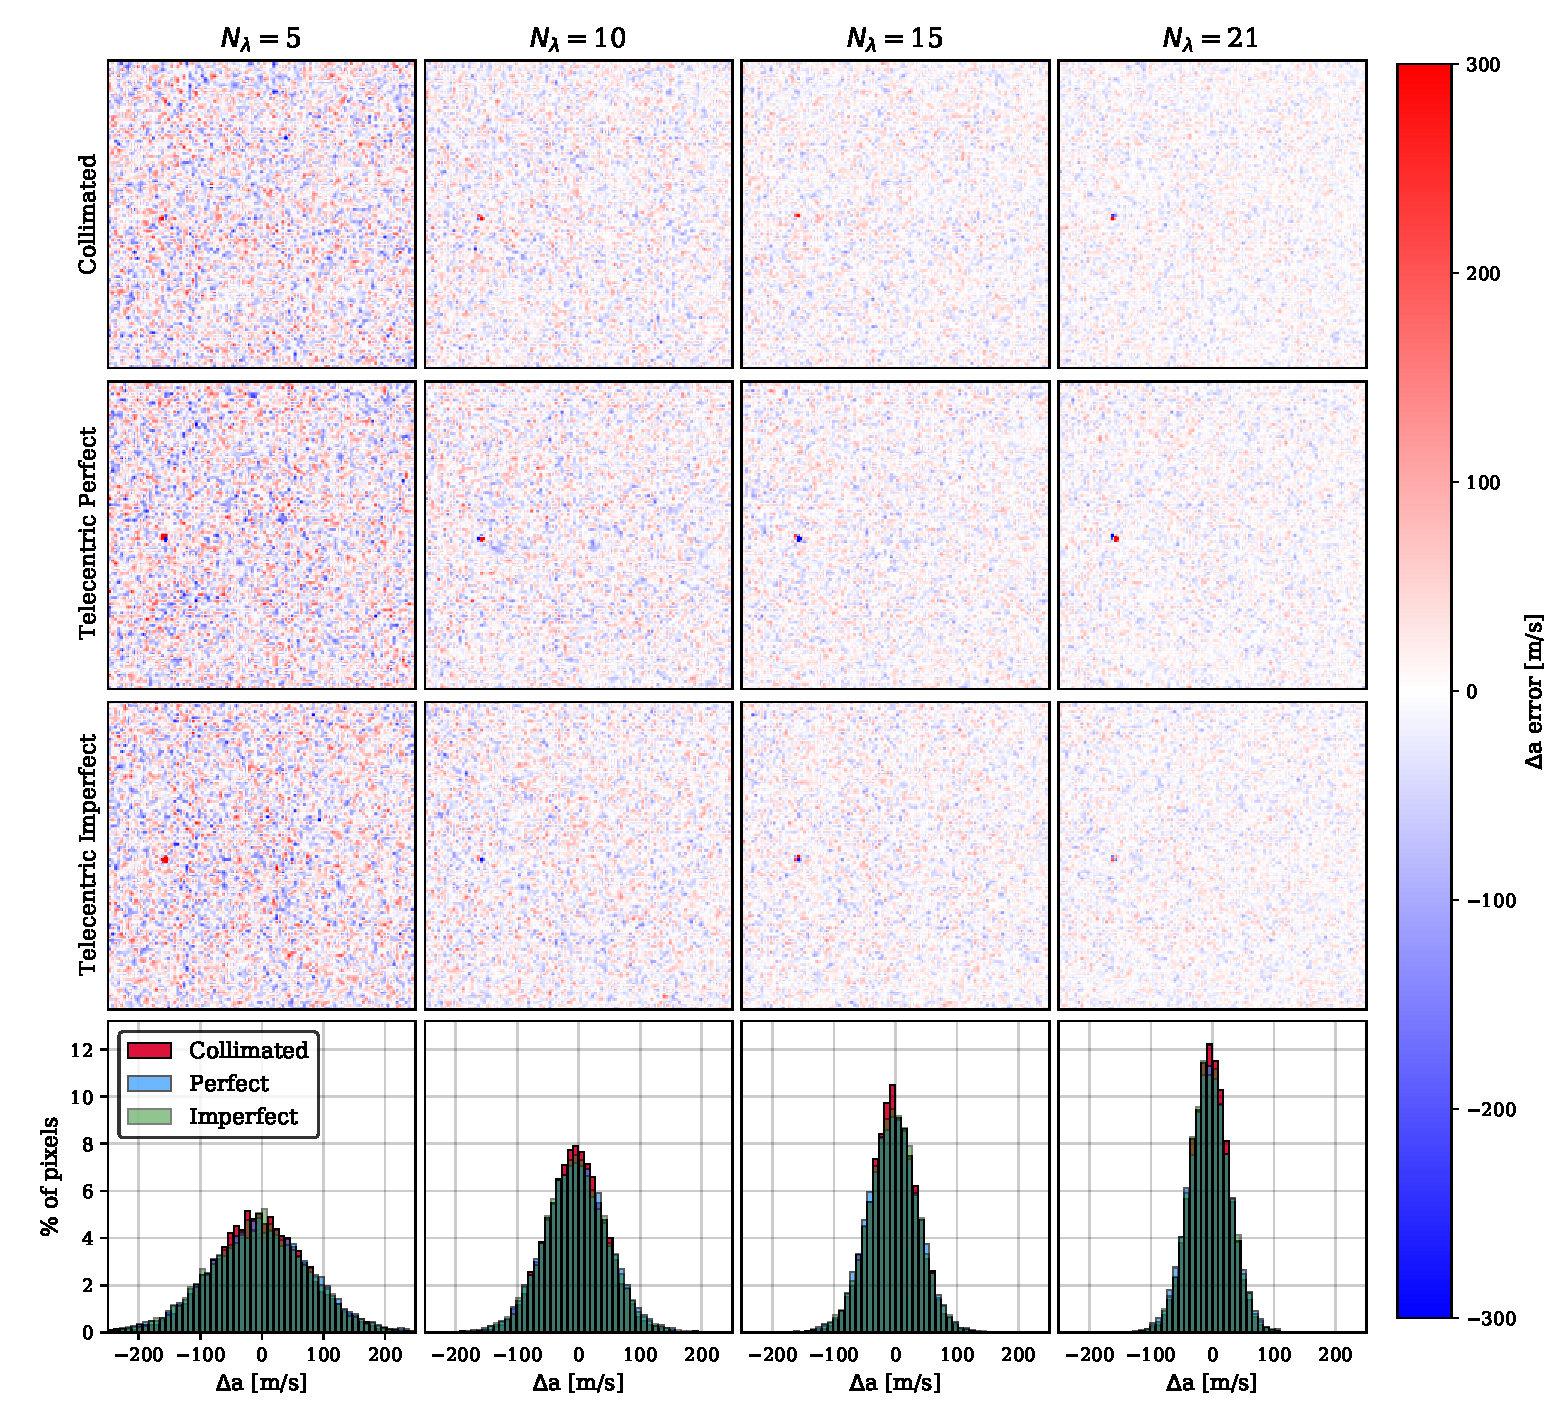
\includegraphics[width=\textwidth]{figures/EtalonPaper/Maps_Fov_Hist.pdf}
    \caption{Distribution of the errors in the $\Delta a$ computation for the three configurations (first three rows) and different spectral samplings (columns). In the bottom panels of each column, the error distribution for the corresponding spectral sampling is shown for the three configurations. }
   \label{fig_etalon_corr:FOV}
\end{figure}

Figure \ref{fig_etalon_corr:FOV} shows the spatial distribution of the errors in the retrieval of $\Delta a$ for different choices of $N_\lambda$. There are no signs of a radial distribution in the maps shown in the figure, contrary to the actual distribution of the $\Delta a$ parameter, as shown in Fig.~\ref{fig_etalon_corr:Inputs}, bottom panel. This means that the precision of the method is similar no matter the amplitude of the defects, that is, we achieve the same accuracy in the retrieval of defects associated with shifts of 3 pm ($\sim$ 1450 ms$^{-1}$, near the corners of our FoV), which correspond to cavity errors of around 1.5 nm or incidence angles of approximately 0.4 degrees, and in the retrieval of regions where no defect is present (radius of 20 pixels from the center of the FoV approximately). Instead of a radial distribution, the errors follow a Gaussian-like distribution (shown at the bottom panels in \ref{fig_etalon_corr:FOV}) similar to the one followed by the noise contribution.

The standard deviation of the errors for both the gain and $\Delta a$ computations are also reduced with an increase in spectral sampling. The last row of Fig. \ref{fig_etalon_corr:FOV} displays the error distributions in the calculation of  $\Delta a$ for the three optical configurations and different spectral samplings. These results illustrate how the three configurations yield practically identical results and how the distribution narrows as $N_\lambda$ increases, thereby improving the results. Specifically, the standard deviation decreases from 50 ms$^{-1}$ for $N_\lambda = 5$ to 20 ms$^{-1}$ for $N_\lambda = 21$. In the case of the gain determination, the standard deviation ranges between 0.2 \% and 0.1\% for the scenarios with the poorest and highest spectral sampling, respectively.

\subsubsection{Impact of the object approximation}

To infer the error of the algorithm when the object is unknown, we compared the performance of the ideal case, that is, when the object used to generate the observations is known, with the one achieved when deconvolving the object from the data. Only the collimated setup was simulated in order to focus exclusively on the errors introduced by the deconvolution. The data has been degraded by Gaussian noise with an S/N = 200 in both scenarios. 

\begin{figure}
    \centering
     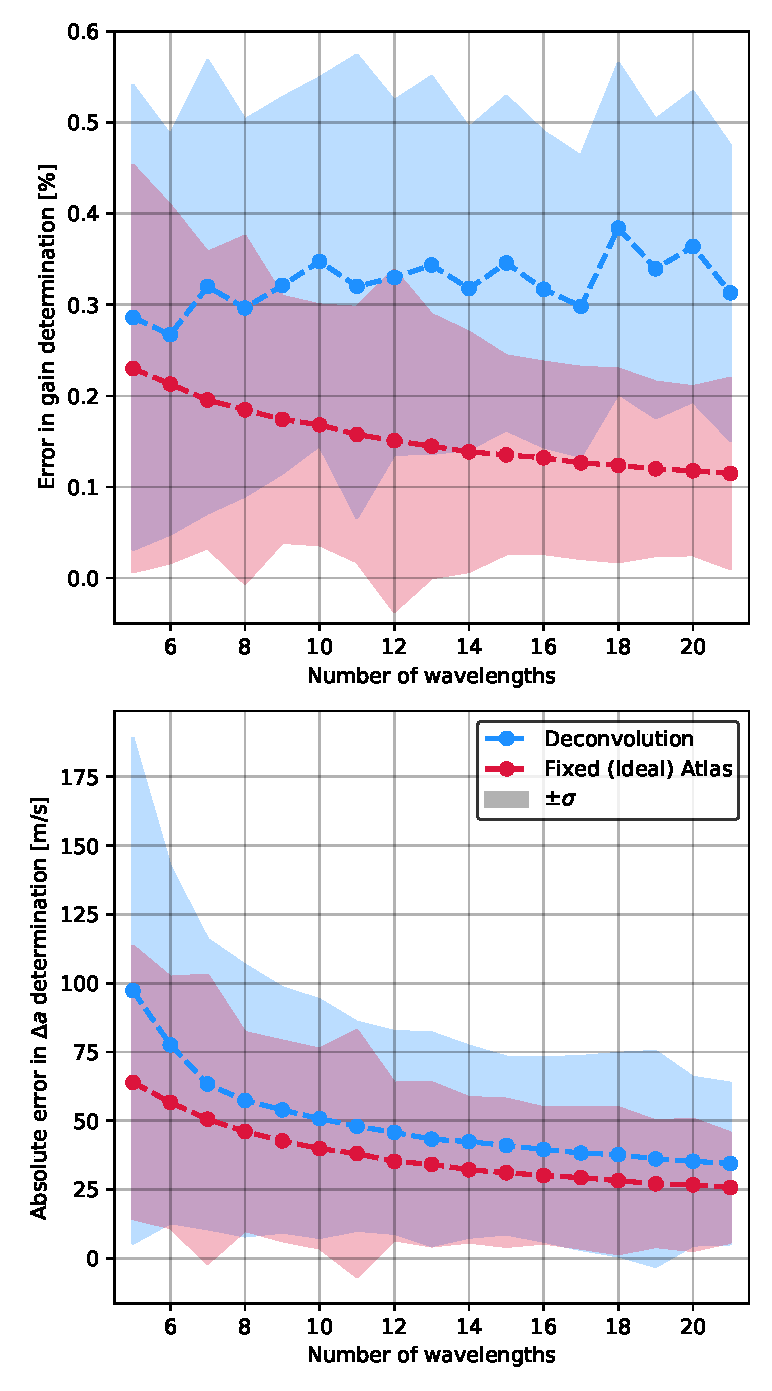
\includegraphics[width=\textwidth]{figures/EtalonPaper/Deconvolution_results.pdf}
    \caption{Errors in gain determination and etalon properties averaged over all the FoV with a signal-to-noise ratio of 200 and a collimated configuration.}
    \label{fig_etalon_corr:Deconvolution-results}
\end{figure}

Figure \ref{fig_etalon_corr:Deconvolution-results} shows the results for the two approaches. Interestingly, the error in the gain for the deconvolution approach does not decrease with a larger number of wavelengths, unlike the ideal case. Nevertheless, the average error of the calculation is below 0.4~\%, with a dispersion (1 $\sigma$) of $\pm$ 0.3~\%. The deconvolution approach is prone to higher errors when deriving the gain due to the normalization of the profiles. The reason for this is two-fold. first, if the continuum is far enough from the spectral line, the normalization is strictly the integral over the transmission profile because the object is flat along the integration interval. However, this is not strictly true since the wings of the transmission profile can reach the spectral line (see Fig.~\ref{fig_etalon_corr:Prof-Measure}), hence modifying the normalization of the profile when the object changes at each iteration. Second, should the continuum intensity of the derived object vary with respect to its real value due to the deconvolution process (e.g., due to boundary effects), there will be a shift in the intensity of the whole profile induced by the normalization process. These two effects seem to dominate the accuracy on the gain determination, regardless of the chosen sampling.

For $\Delta a$, the performance of the method is slightly worse than for the ideal case when using the deconvolution approach. Unlike the gain determination, errors in the $\Delta a$ derivation show a strong dependence on the spectral sampling. Differences between both approaches range from $10$~ms$^{-1}$ to $40$~ms$^{-1}$ and increase with decreasing $N_\lambda$. The sensitivity with $N_\lambda$ is especially high up to $N_\lambda = 8$. A modest increase of $N_\lambda$ from five to six improves the determination of $\Delta a \sim$ 20 ms$^{-1}$, whereas at better spectral samplings, the difference between each simulation decreases more slowly, without any relevant improvement as the sampling increases. In any case, differences are all well within $\pm 1\sigma$.

\subsection{The crossover case}

The fact that the sensitivity of the model to the gain and to the $\Delta a$ parameters are different guarantees (to some extent) that the parameters can be separated from each other. The treatment of the problem is very different between etalon configurations, and therefore full knowledge of the setup is critical. However, this is not always feasible due to the unavoidable presence of errors, misalignment, and imperfections on the instrument. Approximations to describe the optical setup are also common in the pipeline of an FPI instrument because they reduce computational efforts. For instance, telecentric mounts are usually simplified as collimated setups, as the f-numbers employed in solar instruments are usually very large. Imperfections of telecentrism are commonly neglected, too. In this section, we analyze the impact of assuming an incorrect etalon mounting. To do so, we repeated the previous exercise, starting from a perfect and imperfect telecentric configuration but assuming that the transmission profile shape corresponds to a collimated one.    

\begin{figure}
    \begin{minipage}[c]{0.6\textwidth}
      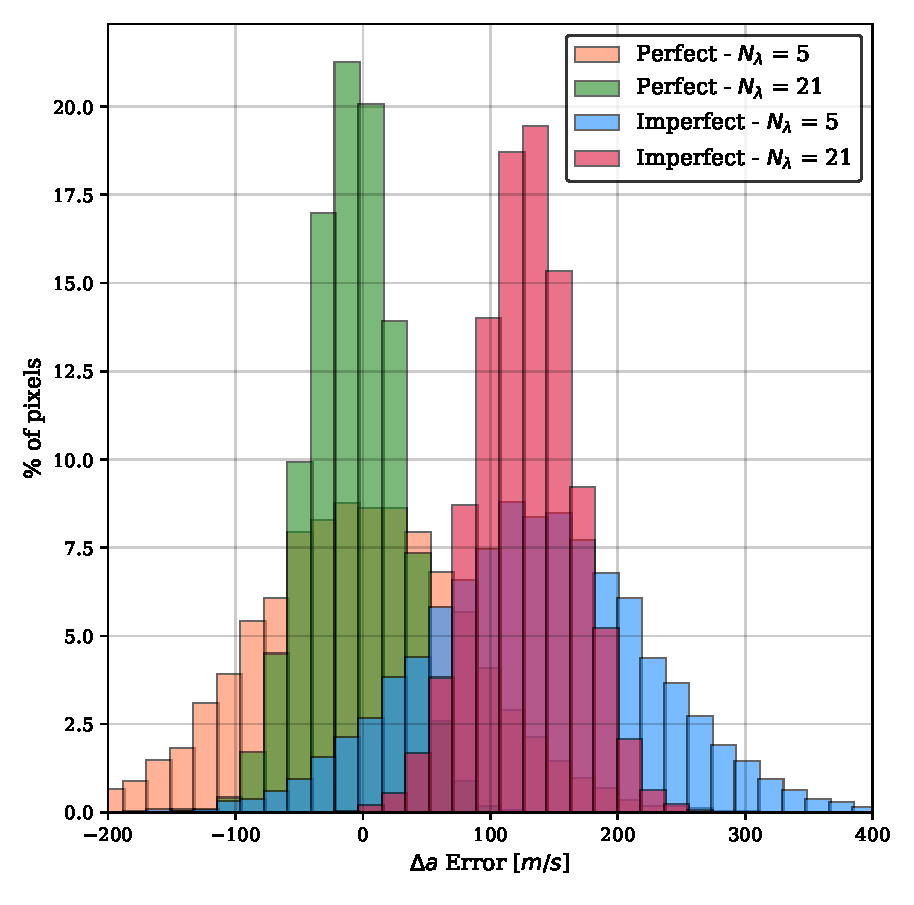
\includegraphics[width=\textwidth]{figures/EtalonPaper/histograms.pdf}
    \end{minipage}\hfill
    \begin{minipage}[c]{0.37\textwidth}
      \caption{
        Distribution of the errors in the determination of $\Delta a$ for the crossover scenarios (different configuration in the observation generation and minimization algorithm) for both perfect and imperfect configurations. Only results for the two extreme spectral samplings ($N_ \lambda = 5$ and $N_\lambda = 21$) are shown.
      } \label{fig_etalon_corr:Crossover_histograms}
    \end{minipage}
  \end{figure}

In this exercise, we assumed that we have an instrument with an FPI in a telecentric mount, as in the previous sections, in both perfect and imperfect configurations and an S/N~$=200$. We also considered that the object is given by the spectral solar atlas. The shift of the perfect telecentric transmission profile with respect to the collimated one was corrected using Eq.52 from \cite{franI} to avoid the emergence of spurious velocity signals. Imperfections in the telecentrism shift the profile more. This additional displacement was left uncorrected intentionally so we could study its effects.

Figure \ref{fig_etalon_corr:Crossover_histograms} shows the error distributions for $\Delta a$ when the model assumes a collimated configuration for $N_\lambda=5$ and $N_\lambda=21$ and for both perfect and imperfect configurations. The amplitude and dispersion of the error distributions are very similar for the two mounts and are comparable to the results obtained in the ideal case (Fig.~\ref{fig_etalon_corr:FOV}, bottom panel). The main difference between the perfect and imperfect scenarios is a shift of $130$ ms$^{-1}$ for the reason mentioned above. We note that this shift can easily be accounted for since it is a known and measurable effect. 

The similarity in the error distributions for the calculation of $\Delta a$ in the two scenarios demonstrates that the error incurred when assuming a collimated etalon does not significantly impact the determination of the cavity maps of the etalon. This is because changes in $\Delta a$ mostly induce a shift of the transmission peak by an equal amount in both cases.


\begin{figure}
  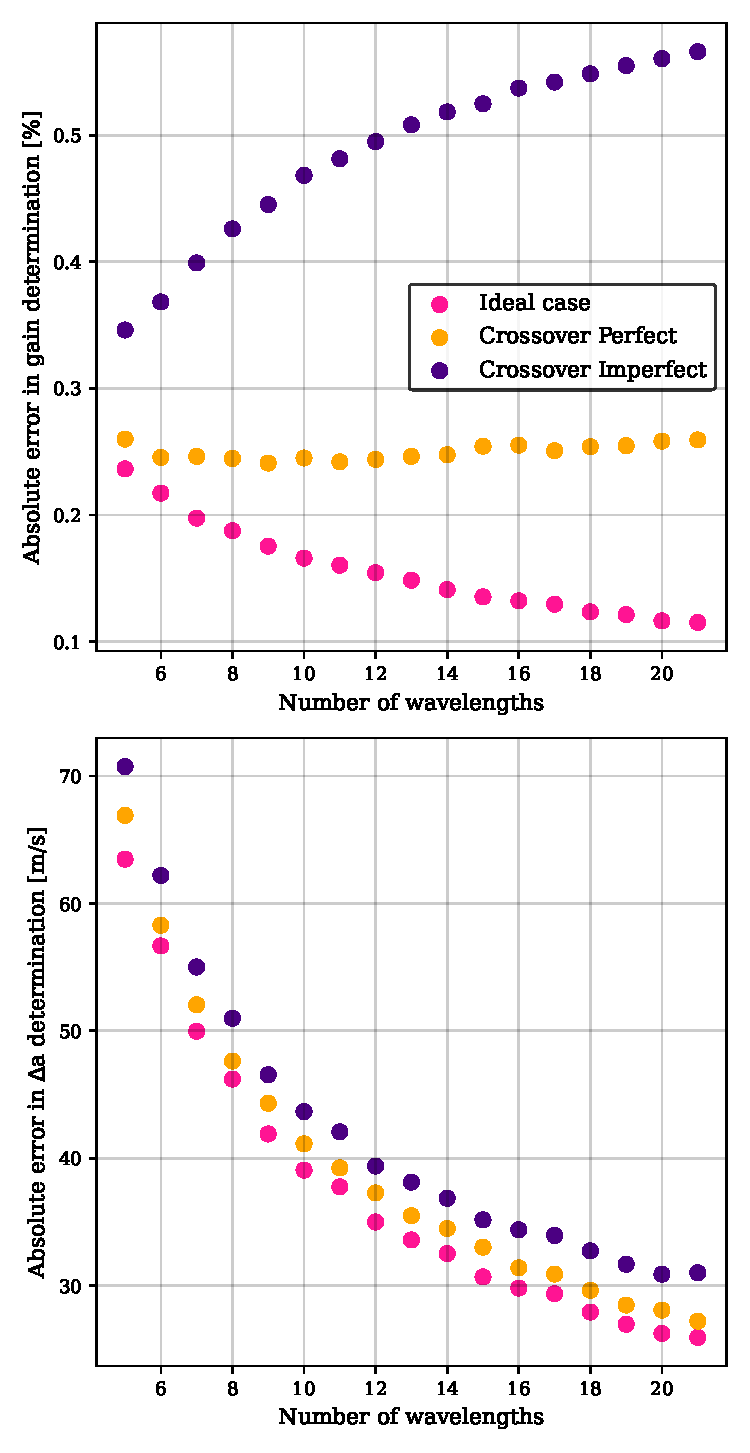
\includegraphics[width=\textwidth]{figures/EtalonPaper/means.pdf}
  \caption{Average errors of the gain (left) and etalon defect (right) calculations over all the FoV for the two crossover cases and the standard case (also shown in Fig.~ \ref{fig_etalon_corr:SNR_both} as the collimated case with S/N = 200) for reference. All $\Delta a$ errors have been computed by correcting differential offsets of the transmission profile between the different mounts.\label{fig_etalon_corr:crossover}}  
\end{figure}

We note, however, that the amplitude, width, and shape of the transmission profile differ significantly between the telecentric and collimated configurations, leading to an expected higher error in gain calculation. Figure \ref{fig_etalon_corr:crossover} shows the absolute errors in gain and $\Delta a$ calculations for both crossover scenarios and the ideal case after correcting the wavelength shift between the different mounts. For $\Delta_a$, the performance of the method is very similar in the three setups, as also observed earlier. This behavior is nevertheless anticipated since the properties selected for simulating the imperfect etalon were chosen to mirror those of the SO-PHI etalon, which were adjusted to closely resemble the behavior of a collimated etalon to the greatest extent possible.

The differences are larger for the gain determination. Not only are the errors higher in the crossover cases, but the trend is entirely different. Instead of decreasing when increasing the number of wavelengths, gain errors remain the same for the perfect case and increase with the number of samples for the imperfect case. Similar to the deconvolution case (Fig.~\ref{fig_etalon_corr:Deconvolution-results}), the difference between transmission profiles introduces an error in the normalization process that systematically affects the rest of the measurements. This effect becomes more pronounced as the number of wavelengths increases, given that this error is introduced more frequently, and it is even more prominent in the imperfect case, as not only are the profiles different in this scenario, but they are also asymmetric. This asymmetry results in an imbalance in the measurement of the profile, as one wing of the spectral line has a higher transmissivity and is observed with greater intensity than the other.

Our results suggest that assuming an etalon in a collimated configuration for instruments with telecentric mounts can be a good first-order approximation for cavity map calculations, provided that the level of asymmetry of the transmission profile is known. However, achieving an accurate knowledge of the degree of telecentrism is often challenging in real instruments, as it usually varies across the FoV. Meanwhile, the results highlight that this approximation leads to a considerable increase in the error in the gain determination, which increases when increasing the spectral sampling. This contrasts with the standard philosophy of solar instrumentation, which requires a high number of points to better scan the spectral line.

% Persistsent homology
%\chapter{\label{CH:Science}Scientific exploitation}


In earlier chapters, we explored data collection and reduction, along with the instrumental challenges involved. Once data have been appropriately reduced, the next step is scientific exploitation, as this is the ultimate goal of all instrumentation.

This chapter presents an example of exploiting spectropolarimetric data through the study of magnetic field intensity maps, or magnetograms, recorded with both Hinode/SOT and SDO/HMI. Aligned with the computational focus of this thesis, we apply a novel data processing approach for studying solar magnetograms: a topological data analysis technique known as persistent homology. The research in this chapter stems from work completed during a two-month stay at NAOJ between the first and second Sunrise III flights, leading to the publication of the article "Persistent Homology Analysis for Solar Magnetograms" \citep{PH_yo}. Again, since this work was done before the successful flight of Sunrise III, the lack of TuMag data required us to use different instruments.

We begin by discussing the motivation for introducing new techniques in solar magnetogram analysis and the specific benefits of persistent homology. A general overview of the method follows, introducing the tools it provides. Finally, we present our analysis, illustrating how persistent homology helps characterize magnetic structures and dynamics in both quiet Sun regions and active regions.

\section{Persistent Homology in Solar Magnetograms.}
The ability to encode and simplify all information about the shape and distribution of data has made Topological Data Analysis (TDA) one of the most relevant fields in state-of-the-art data analysis. In recent years, we have witnessed a rise of studies based on TDA techniques in many fields of science, such as biomedicine \citep{brain-PH}, atomic physics \citep{atomic}, image recognition \citep{Image-recognition} or cosmology \citep{cosmology}, among many others.

Among the numerous techniques of TDA, persistent homology is arguably the most widely used approach for studying real data. By examining the persistence of topological features, persistent homology can identify significant structures present at different scales, and at the same time, its performance is very robust against noisy and/or incomplete data \citep{PH_noisy}. Furthermore, persistent homology provides a straightforward and intuitive way for the visualization of the results. This simplifies the interpretation of the results, while also serving as a good descriptor of the data's topological properties, therefore making it a suitable input for machine learning algorithms.

The application of these techniques in solar observations presents a promising approach to understand the complex structures and dynamics of the Sun's behavior. Specifically, the analysis of the solar magnetic field using magnetograms is particularly well-suited for the application of these methodologies, given the intricate and multi-scale nature of the magnetic structures. Solar magnetograms provide a visual and quantitative representation of the magnetic field in the photosphere and are one of the fundamental tools for the study of our star. The magnetic activity of the Sun is very diverse, from the quieter events occurring in the quiet Sun to the more violent and extreme events like solar flares and coronal mass ejections (CMEs) in active regions. In this sense, magnetograms are very useful as they enable us to study all these events through magnetic field measurements.

Numerous studies utilize magnetograms to investigate the behavior of solar magnetic fields. The intricate nature of the magnetic structures has led to the development of various techniques, each tailored to focus on distinct properties of the magnetic field. One of these techniques is the study of the power spectrum of magnetograms through Fourier transforms, as employed in numerous works: in \cite{power_spectrum1}, where they attempt to establish a correlation between the magnetogram power spectrum and flare production; in \cite{power_spectrum_2}, where they use the magnetogram power spectrum to study the quiet-sun turbulence; in \cite{power_spectrum_3}, where they analyzed the power spectrum of different physical quantities and study their dependence with the total magnetic flux; or in  \cite{power_spectrum_4}, where they tried to reproduce the magnetograms power spectrum through simulations, among other instances. 

Different approaches are also common. Some examples of alternative methodologies can be found in: \cite{intermitency}, where they study the intermittency and multifractality of the magnetic structures and their relation with flaring activity; in \cite{conectivity}, where they study the magnetic connectivity to define a criteria for the distinction of flaring and nonflaring regions; or in \cite{gosic}, where they analyze long time series of magnetograms with high cadence and spatial resolution to calculate the number of field appearances and cancellations, as well as their interactions, to determine the net magnetic fluxes on the Sun's surface; among many other approaches in the field.

The increasing volume of data generated by modern instruments highlights the growing importance of data analysis techniques. Many studies have directed their efforts towards the development of automatic feature detection and tracking algorithms for solar magnetograms. Prominent examples of widely employed approaches for Quiet Sun studies include SWAMIS\footnote{The Southwest Automatic Magnetic Identification Suite} \citep{swamis_yafta}, as employed, for example, in \cite{swamis_example}, where they employ the code to track the magnetic elements and study the flux dispersal in the Quiet Sun. Another example is YAFTA\footnote{Yet Another Feature Tracking Algorithm} \citep{yafta}, employed in \cite{yafta_example},  where they track the proper motion of magnetic elements of the Quiet Sun to study the dynamics of supergranular flows. Concerning active regions, there have been numerous works on the matter of classification and detection methods, from the well-known, and classical approach of the Mount-Wilson classification \citep{hale}, to more recent contributions, such as the SHARP\footnote{Spaceweather HMI Active Region Patch} tool \citep{sharp}, that has emerged as one of the most prominent algorithms for this purpose.

Although these studies provide valuable insight into the processes occurring in the photosphere and the interrelations of the solar magnetic field with other solar phenomena, the underlying governing laws remain highly complex and challenging to fully ascertain. The integration of TDA techniques into these analyses has the potential to offer a previously unexplored perspective on these phenomena that complements the current knowledge. Persistent homology algorithms share similar methodologies (such as image thresholding) with other feature detection/tracking codes like SWAMIS or YAFTA. However, unlike these codes, persistent homology provides topological information about the detected features and employs it to discern between different types of structures. This includes information on the connectivity to neighboring features, the shape of the feature, and the presence or absence of holes in the magnetic feature. All this information allows persistent homology to distinguish between different types of magnetic features based on their topological properties, and to identify and track the presence of a particular type of magnetic structure. In addition, since these algorithms can identify the pixels that make up each topological feature, they can be used to outline magnetic elements and facilitate conventional calculations such as determining the size or flux of magnetic structures.

In particular, topological techniques can be particularly useful for studies related to solar flares. It is well known that active regions exhibiting intricate structures are linked to the occurrence of solar flares. Three critical factors establish a connection between the characteristics of active regions and flare production: surface area, magnetic complexity, and rapid temporal evolution \citep{flare_LR}. While the first factor is straightforward to measure (e.g., the sunspot area and total unsigned magnetic flux), persistent homology techniques may enable topological quantification of the latter two, which present greater challenges when utilizing conventional methods. Some studies have already delved into this concept; for example, in \cite{ph_solar_2}, they employ a persistent homology analysis to explore the predictive capabilities of a machine learning model for the forecasting of solar flares based on the topological information extracted from solar magnetograms. However, they did not study the correspondence between the magnetic features and the topological information extracted from persistent homology, which is the main focus of this work.



\subsection{Persistent Homology}

Persistent homology stands out as a prominent technique within the topological data analysis toolkit, primarily for its capacity to capture the shape and distribution information of a dataset. The algorithm is rooted in the mathematical framework of homology groups. In topology, these groups measure the number of $n$-dimensional holes in a data set, or in other words, the number of connected components for a  $0^{th}$ dimensional analysis, holes or rings for a $1^{st}$ dimensional analysis, spherical voids for the $2^{nd}$ dimensional analysis, and so on. 

The primary objective of persistent homology is not only to compute the homology groups of a given dataset but also to study how they vary at different scales. To achieve this, the input data undergoes a process of division into a series of sequential subspaces, with each subspace encompassing the previous one. This sequential process, known as filtration, begins with a starting subspace comprising a single point from the original dataset. Subsequent subspaces are then constructed by incrementally adding points to the previous subspace until the final subspace includes all points of the original dataset. 

After the filtration process is performed, persistent homology algorithms shift their focus to analyzing the evolution of topological features across the different subspaces. Specifically, they record the filtration value at which a new feature appears, meaning that it is absent in the previous subspace, and when it disappears, meaning that it is no longer present in the following subspaces. These two events are known as the birth and death of a topological feature, respectively. 

In a nutshell, the $n$-dimensional persistent homology of a dataset with a given filtration can be described as the aggregation of all n-dimensional features (homology groups) that were created (birth) and subsequently eliminated (death) during the filtration process \citep{ph_filtration}.

When applying persistent homology on a greyscale image, our focus lies in filtering the data according to the pixel values. Multiple filtering approaches exist, with the most extended ones being sublevel and superlevel filtrations, both based on the concept of thresholding. In these filtrations, the image is cropped to a specific value, forming a subspace that includes all pixels with values higher than this value in a superlevel filtration, or lower in a sublevel filtration. This cropping value (i.e. the filtration value) is systematically varied from the lowest to the highest values of the image, or vice versa, thus generating a different subspace for each value. As a result, the persistence homology analysis captures and examines the evolution of topological features across different thresholds, enabling insights into the image's structural properties at various scales \citep{ph_image_filtration}.

A more formal way of defining these filtrations can be done by considering an image as a discrete representation of a function $f$, defined over a two-dimensional space $\mathbb{X}$, such that: 
\begin{equation}
    f :  \mathbb{X} \longrightarrow  \mathbb{R} \ \ .
\end{equation}
Let $\mathbb{S} _\phi$ be the subspace of $\mathbb{X}$ for a filtration value of $\phi$. In such a case, a filtration can be expressed as:
\begin{equation}
    \mathbb{X}: \mathbb{S}_{\phi_0} \subset \mathbb{S}_{\phi_1} \subset \mathbb{S}_{\phi_2}\subset... \subset \mathbb{X}\ \ .
\end{equation}
With this formulation, a topological feature with birth-death coordinates:
\begin{equation}
(B, D) = (\phi_ I, \phi _ {II}) \ \ ,
\end{equation} 
corresponds to a feature that appears for the first time during the filtration process at the subspace $\mathbb{S}_{\phi _ I}$, and \textit{persists} until the subspace $\mathbb{S}_{\phi _ {II}}$, where it ceases to exist.

In a sublevel filtration, each subspace can be expressed as:
\begin{equation}
    \mathbb{S} _ \phi = f ^{-1} \left( ( -\infty, \phi ] \right) \ \ ,
    \label{eq: sublevel}
\end{equation}
where $\phi_0$ is selected as the lowest value for any given pixel and its value is increased until the subspace includes all pixels. On the contrary, in a superlevel filtration, the subspaces can be expressed as:
\begin{equation}
    \mathbb{S} _ \phi = f ^{-1} \left( [ \phi, \infty ) \right)\ \ , 
    \label{eq : superlevel}
\end{equation}
where $\phi_0$ is selected as the highest value for any given pixel and its value is decreased along the filtration.

Various methods exist for representing the information derived from a persistent homology analysis, including Betti numbers, persistence bars, and persistent diagrams (PDs) (\citealt{pd_stability}, \citealt{pbars}), among many others. For this study, we will utilize the PDs as our chosen approach due to their straightforward interpretation and extended use. A $n$-dimensional PD is a multiset of Birth-Death pairs, ($B _ i, D _ j$), with multiplicity $k$, where each pair measures the number ($k$) of $n$-dimensional components that have been born at the filtration subspace $\mathbb{X}_i$ and died in $\mathbb{X}_j$, that is usually represented in a 2D scatter plot. 

\begin{figure}
    \begin{minipage}[c]{0.67\textwidth}
      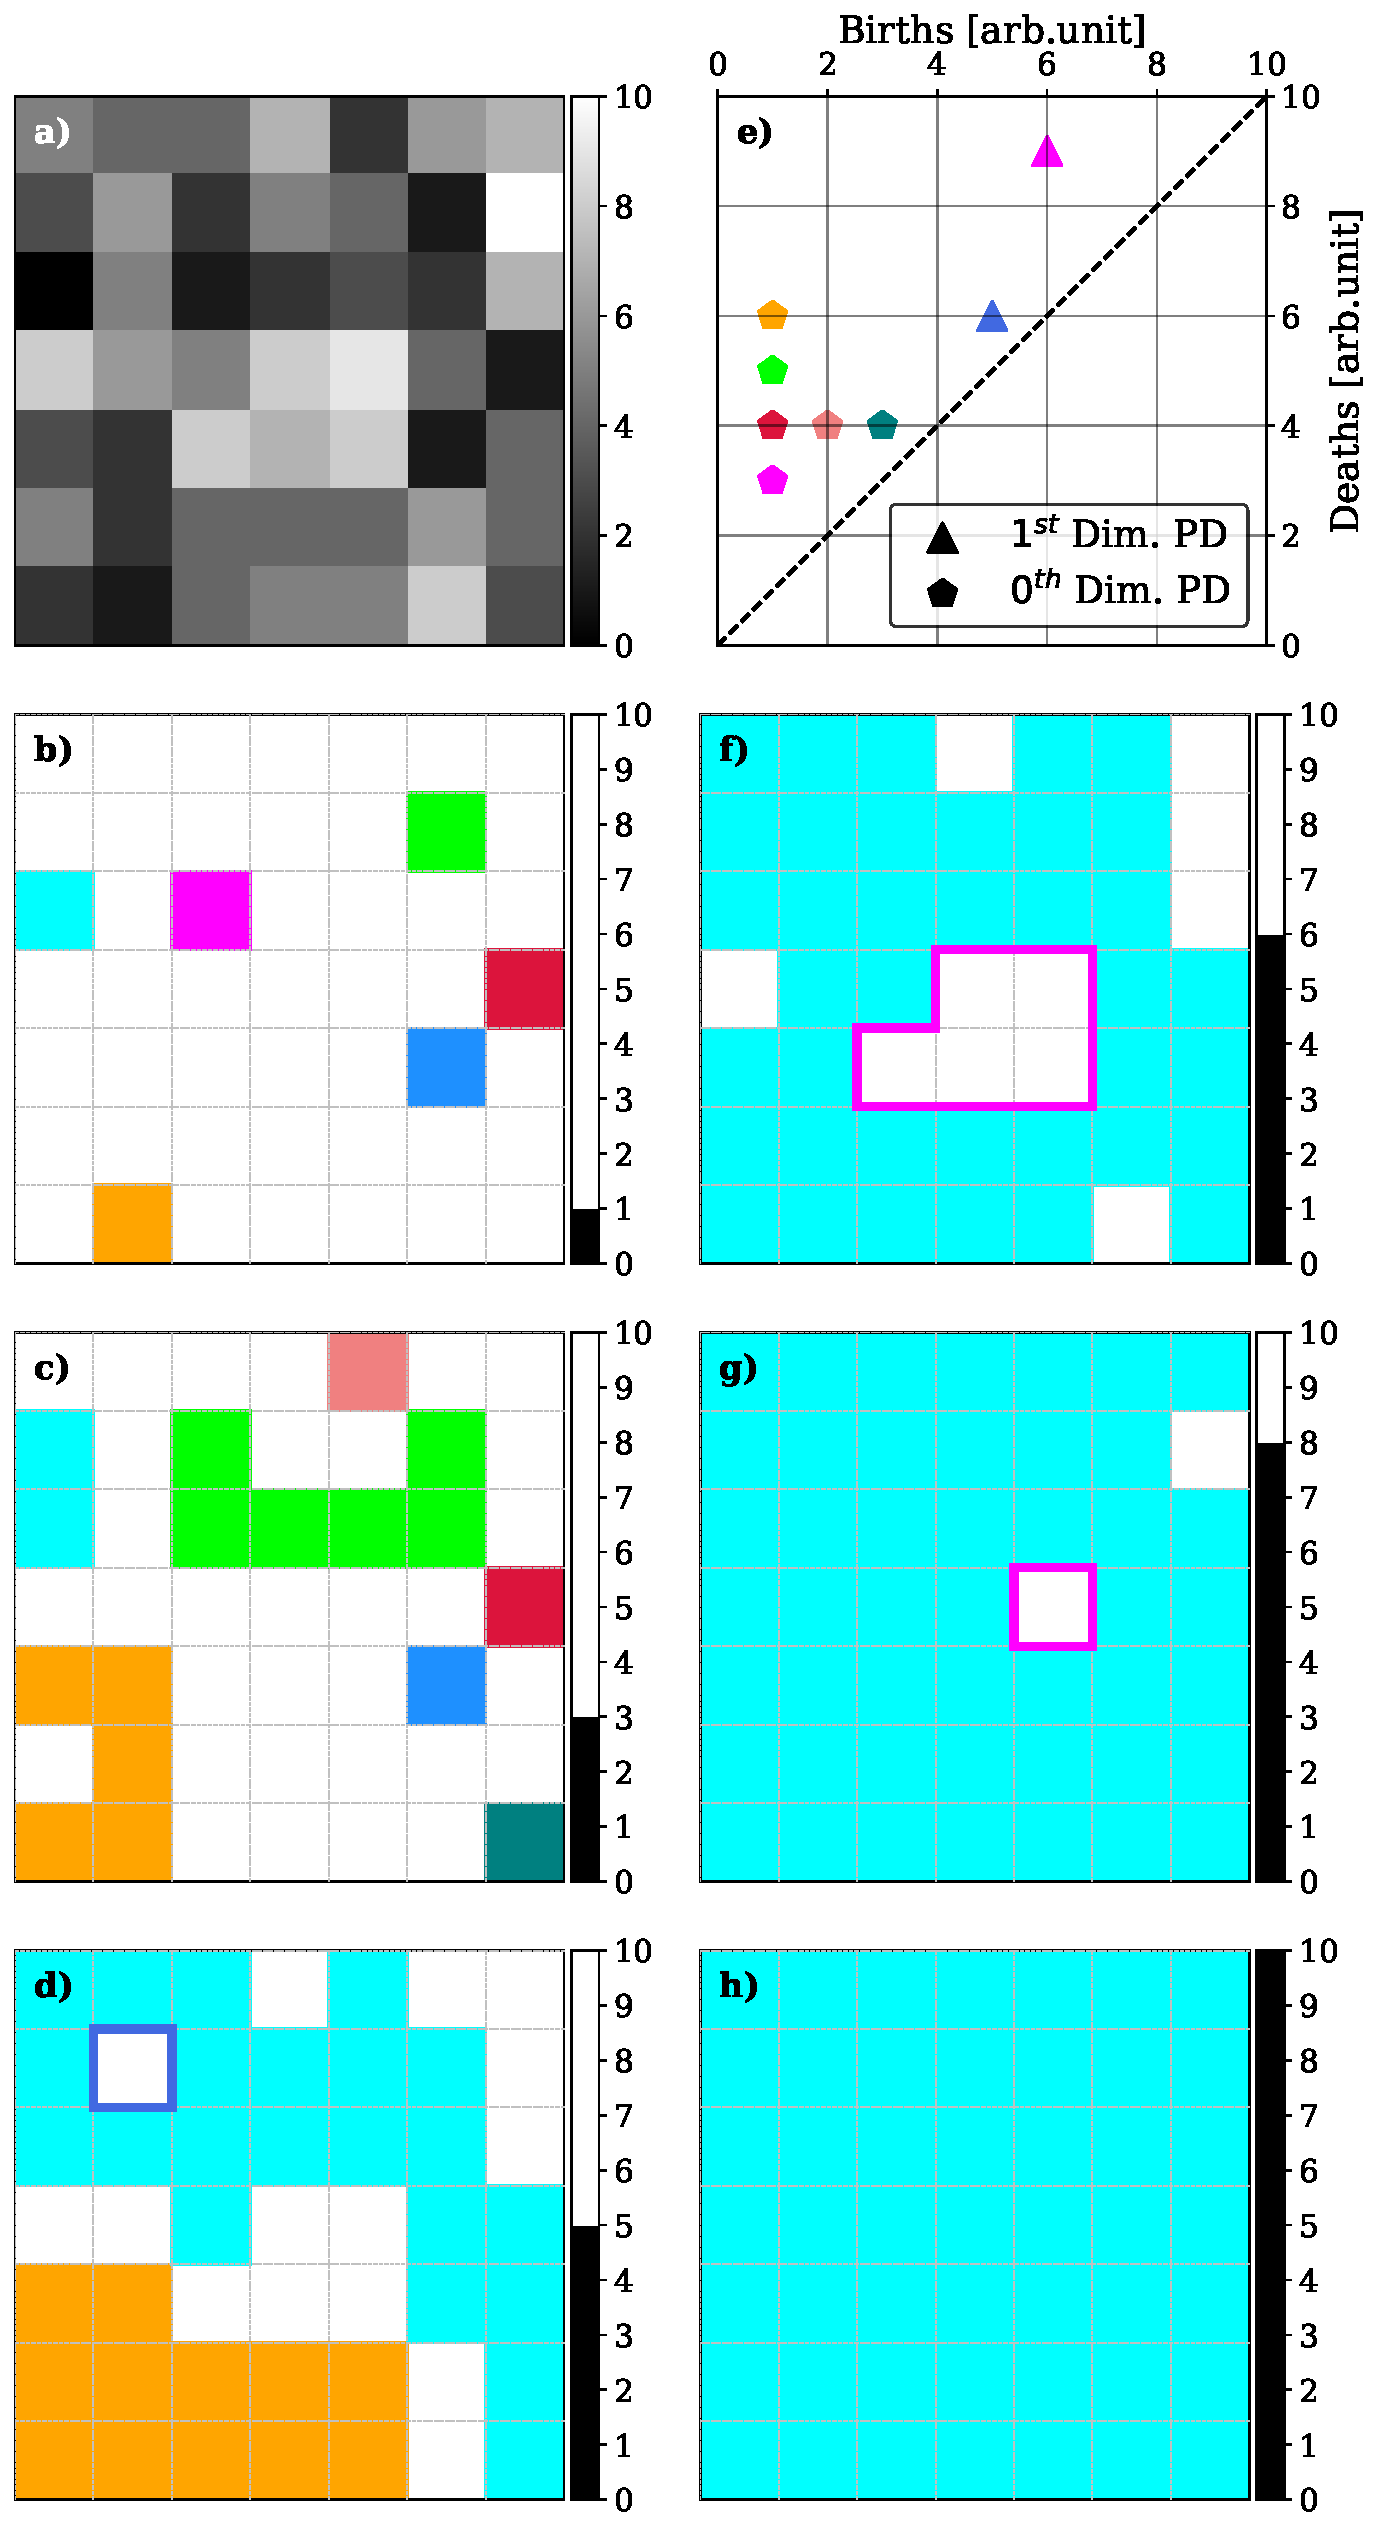
\includegraphics[width=\textwidth]{figures/PersistentHomology/ImageFiltering_example_v.pdf}
    \end{minipage}\hfill
    \begin{minipage}[c]{0.3\textwidth}
      \caption[Grayscale image sublevel filtration example.]{
        Sublevel filtration of a greyscale image and PDs of the $0^{th}$ and $1^{st}$ dimensions. Panel a) shows the input data. In panels b), c), d), f), g), and h) different snapshots of the filtration process are shown. The value of the filtration parameter, $\phi$ is shown in the color bar at the right of each image. Only pixels with a value lower than the filtration value (colored pixels) belong to the subspace shown in each snapshot. Different homology groups are represented with different colors at each snapshot. For connected components ($0^{th}$ dimensional homology groups) the whole pixel is shown with the corresponding color. For rings, ($1^{st}$ dimensional homology groups), only the border of each hole is colored. In panel e) the PDs of both dimensions are shown. The color of each point in the diagram is the same as the one used to plot the corresponding topological feature in other panels.
      } \label{fig_ph: Image Filtration Example}
    \end{minipage}
  \end{figure}

The process of generating a PD of a greyscale image is as follows. We start by selecting the filtration direction (sublevel or superlevel) and the dimension of the analysis (either 0 or 1). We initialize a threshold as the highest or lowest value from the image, depending on the choice of filtration. We then perform the filtration by systematically adjusting the threshold and creating a binary image for each threshold. This process divides the image into two sets: pixels with values matching or above the threshold and pixels with values below it. The choice of filtering determines which of the two sets makes up the subspace. We then look for the existing topological features within each of these subdivisions. The specific process by which these features are identified is detailed in the next paragraph, where the structures corresponding to both dimensions are illustrated using the example shown in Fig.~\ref{fig_ph: Image Filtration Example}. We repeat this process until the threshold reaches the opposite limit to that from which it started. Along this process, we follow the appearance, merging, and disappearance of connected components. When two components merge, the longer-lived one (\textit{i.e}. the first to appear along the filtration process) absorbs the younger one, thus resulting in the death of the second \citep{eldest}. We determine the birth and death for each component based on the thresholds at which these events occur.  Finally, we construct a scatter plot where the horizontal axis represents the birth values and the vertical axis represents the death values. Each point on this plot corresponds to a persistence point, whose coordinates reveal the scales at which the corresponding topological feature is present.

An example of this process with a sublevel filtration is shown in Fig.~\ref{fig_ph: Image Filtration Example}. Panel a) displays the input data, panels b), c), d), f), g), and h) show some of the key steps of the filtration process, and, lastly, panel e) displays the PD for a $0^{th}$ and $1^{st}$ dimensional analyses. These plots illustrate how connected components and rings are born and then die as we increase the filtration level. As these components (shown in different colors) increase in size and come into contact with other components, one absorbs the other, thus resulting in the death of the second. This phenomenon is shown in panels b) to d), where we observe the progression of the components until only the blue and orange connected components remain. Additionally, the diagrams also reveal the appearance of two rings in the data (panels f) and g)). These rings are found when pixels that do not belong to the subspace are surrounded by a connected component, and die when those pixels are included in the component as the threshold increases (blue ring in panel d)). Finally, the PD (panel e)) displays the birth and death values (i.e. the filtration value) of all the features, of dimensions 0 and 1, that have been identified (birth) and subsequently eliminated (death) throughout the filtration process. 

\subsection{Persistent Images}

The PD displayed in Fig.~\ref{fig_ph: Image Filtration Example} contains only a limited number of points due to the simplicity of the input image. However, when analyzing real data, these diagrams can consist of hundreds or even thousands of birth-death pairs with high multiplicities, simply due to the size of the images. Additionally, features not only representing the genuine behavior of the data but also reflecting the distribution of noise appear on the diagrams. To address this complexity, several strategies have been developed to simplify the information from PDs, such as persistence curves  \citep{persistence_curves}, persistence landscapes \citep{persistence_landscapes}, or persistence images (PI) \citep{persistence_images}. In this study, we will focus on the latter, due to its noise filtering capabilities and because the representation of the results remains in a Birth-Death diagram, allowing for easy interpretation of the results, similar to a persistence diagram.

PIs are a condensed form of a persistence diagram, offering a concise and easy-to-understand representation of its topological features.  They capture the spatial distribution and persistence information of these features, allowing for the enhancement of the most relevant ones and filtering of the others. A PI is constructed using the concept of persistence. Each topological feature, represented by a point in a PD, has a persistence, $\pi$, of:

\begin{equation}
    \pi = D - B
    \label{eq: persistence}
\end{equation}


where $(B, D)$ are the corresponding birth-death coordinates in the diagram. A feature with a large persistence is present at different scales in the data and therefore is more likely to represent the real behavior of the data. On the contrary, short-lived features are typically associated with the noise distribution and usually do not provide much information about the data.

\begin{figure}
  \begin{minipage}[c]{0.67\textwidth}
    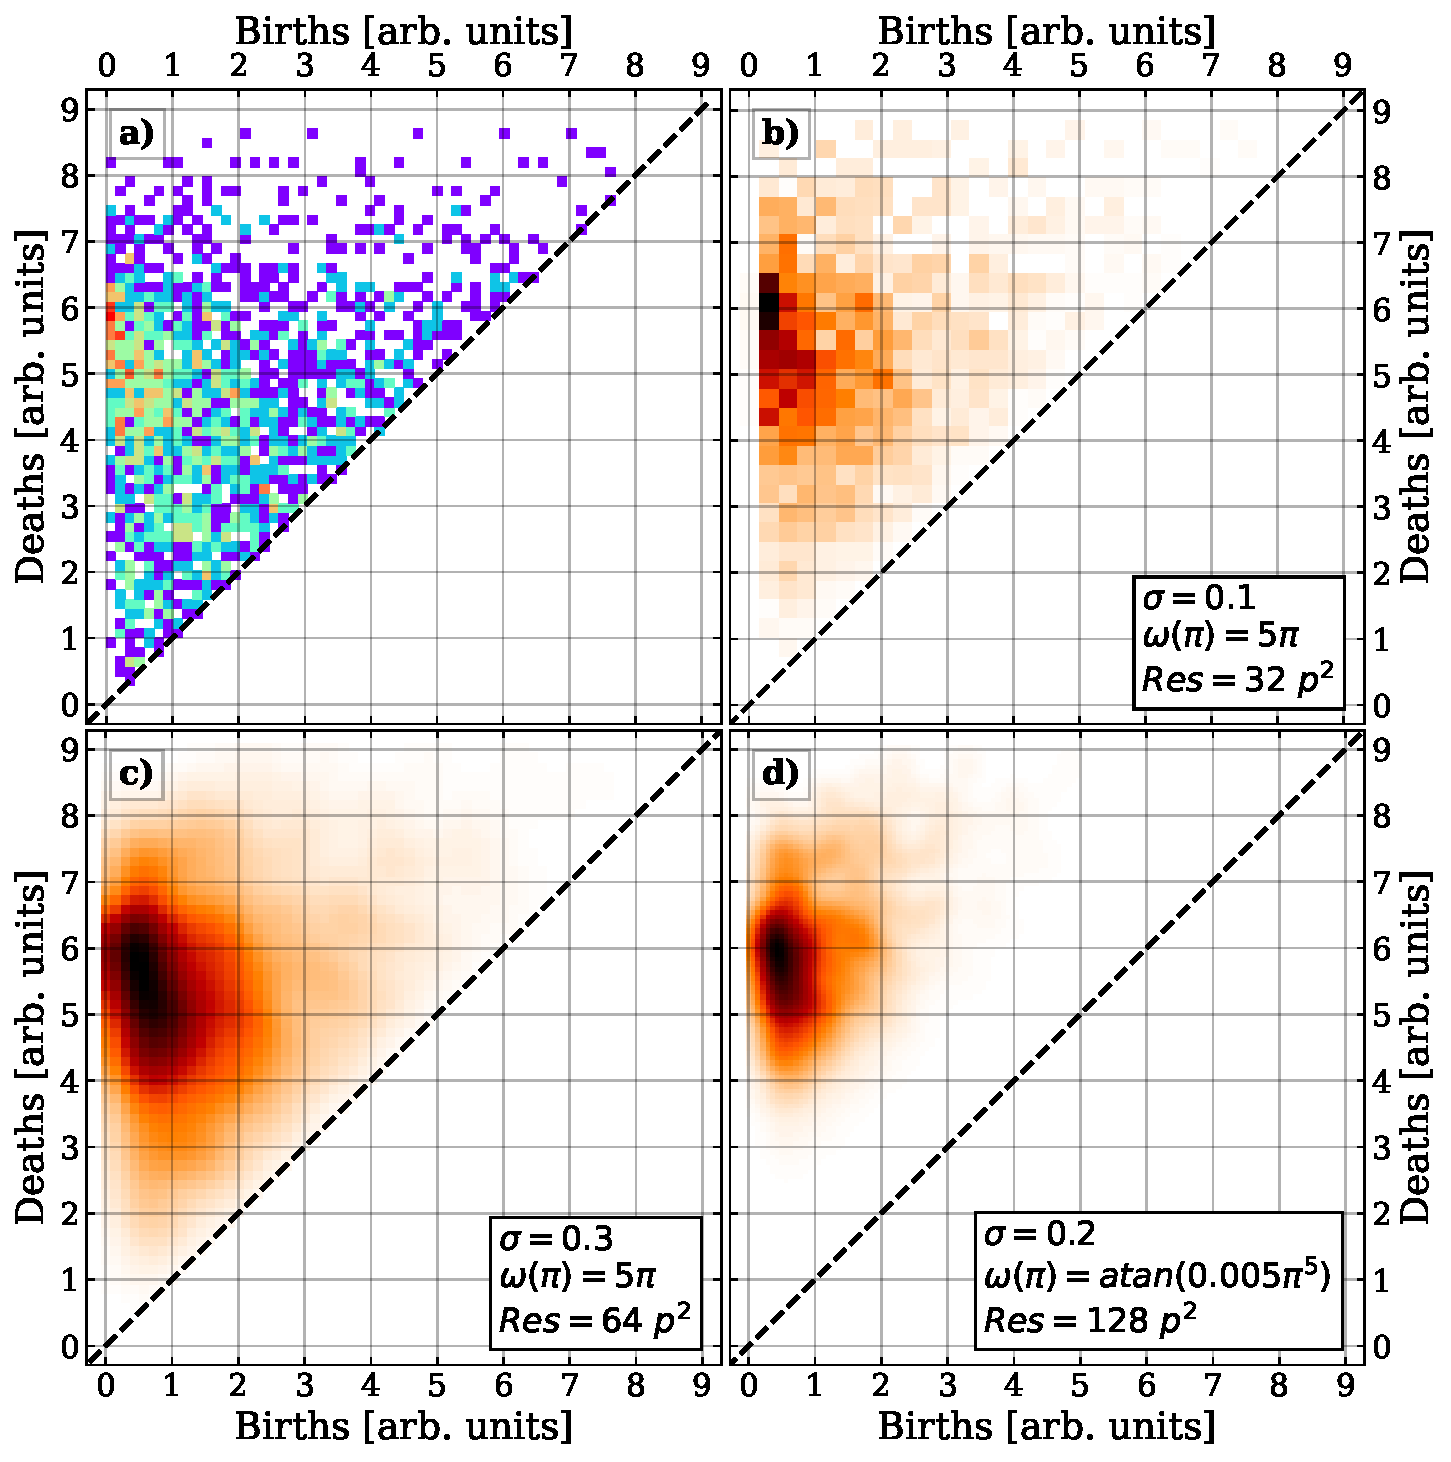
\includegraphics[width=\textwidth]{figures/PersistentHomology/PI_Example.pdf}
  \end{minipage}\hfill
  \begin{minipage}[c]{0.3\textwidth}
    \caption[Persistent image examples.]{Panel a) shows an example of a persistence diagram as a 2D histogram. The color of each bin represents its multiplicity, with the red spots corresponding to higher values. Panels b), c), and d) show three different examples of PIs. The three parameters given in the legends of the PIs are: the standard deviation ($\sigma$) of the Gaussian kernel ($K (z)$), the weighting function, and the resolution of the image PI in pixels (p).}
   \label{fig_ph: PI Example}
  \end{minipage}
\end{figure}

When constructing a PI, a weighting function, $\omega (\pi)$, is employed to assign weights to each point in the diagram, ensuring that longer-lived features have greater weights than shorter-lived ones. There are multiple choices for the shape of the weighting function, which are entirely dependent on the aims of the study and data type. The simplest example is often a linear or power-law relation ($\omega (\pi) = a \pi ^b$), where $a$ and $b$ can be tuned to assign progressively higher weights to higher persistencies, thus focusing the study on the longer-lived components. On the other hand, if the objective is to filter out noise while assigning similar weights to all non-noise points so that all points have a similar relevance in the analysis, the chosen function is usually an arc-tangent.

The PI is then generated by dividing the persistence diagram plane into a grid with a desired resolution. Within each grid region (or pixel), the weighted features of the diagram within the region are added up using a kernel density estimation. The kernel function, $K (z)$, can be tuned to suit the nature and objectives of the analysis, with Gaussian functions being the most common approach. 

The resultant PI is a 2D matrix, wherein each pixel corresponds to a specific area in the persistence diagram, and its value represents the cumulative weight of the topological features found within that area. In Figure \ref{fig_ph: PI Example}, three examples of PI (panels b), c), and d)) are presented for the same persistence diagram (panel a)), where distinct choices of resolution, kernel function, and weighting function have been applied to each image.




All the PDs, PIs, and the rest of the analysis tools presented in this work, have been computed using the Homcloud python package \citep{homcloud}.


\subsection{Data}

In this work, we study the results of applying persistent homology to different regimes of solar activity by applying the analysis to both quiet Sun and active region magnetograms.

\subsubsection{Quiet Sun observations}

The study of quiet Sun regions requires high magnetic spatial and temporal resolutions and sensitivities to be able to capture the small-scale evolution of the magnetic structures due to their weak signals ans short time scales \citep{quiet_sun_living_review}. For this reason, we employ observations taken by the Solar Optical Telescope (SOT; \citealt{sot}) aboard the \textit{Hinode} satellite \citep{Hinode}, a space-borne solar observatory. In particular, we employ observations from Hinode's Operation Plan (HOP) 151. These observations consist of long ($\ge 20$ h) and mostly uninterrupted sequences of measurements of the Narrowband Filter Imager of the Na I D1 line at 5896 \r{A} taken with a cadence of $50-70$ s. The data correction of the selected observation sets has been carried out in \cite{gosic}.


\subsubsection{Active regions observations}

We employ observations of active regions (ARs) taken by the Helioseismic and Magnetic Imager (HMI; \citealt{hmi1}, \citealt{hmi2}) on board the Solar Dynamics Observatory \citep{SDO}. HMI provides a continuous observation of the Sun where a full-disk magnetogram, as well as Dopplergrams, are provided at all times. The full-disk, uninterrupted observations of HMI make it a very suitable instrument to study the evolution of active regions as the formation and development of active regions can be fully captured. 

We focus the analysis on a series of newly-emerging ARs identified in \citep{toriumi}. In particular, we employed the 12-minute cadence observations taken during the period from May 2010 to June 2011, which corresponded to a period of low solar activity.

\subsection{Analysis and results}

\begin{figure}
    \centering
     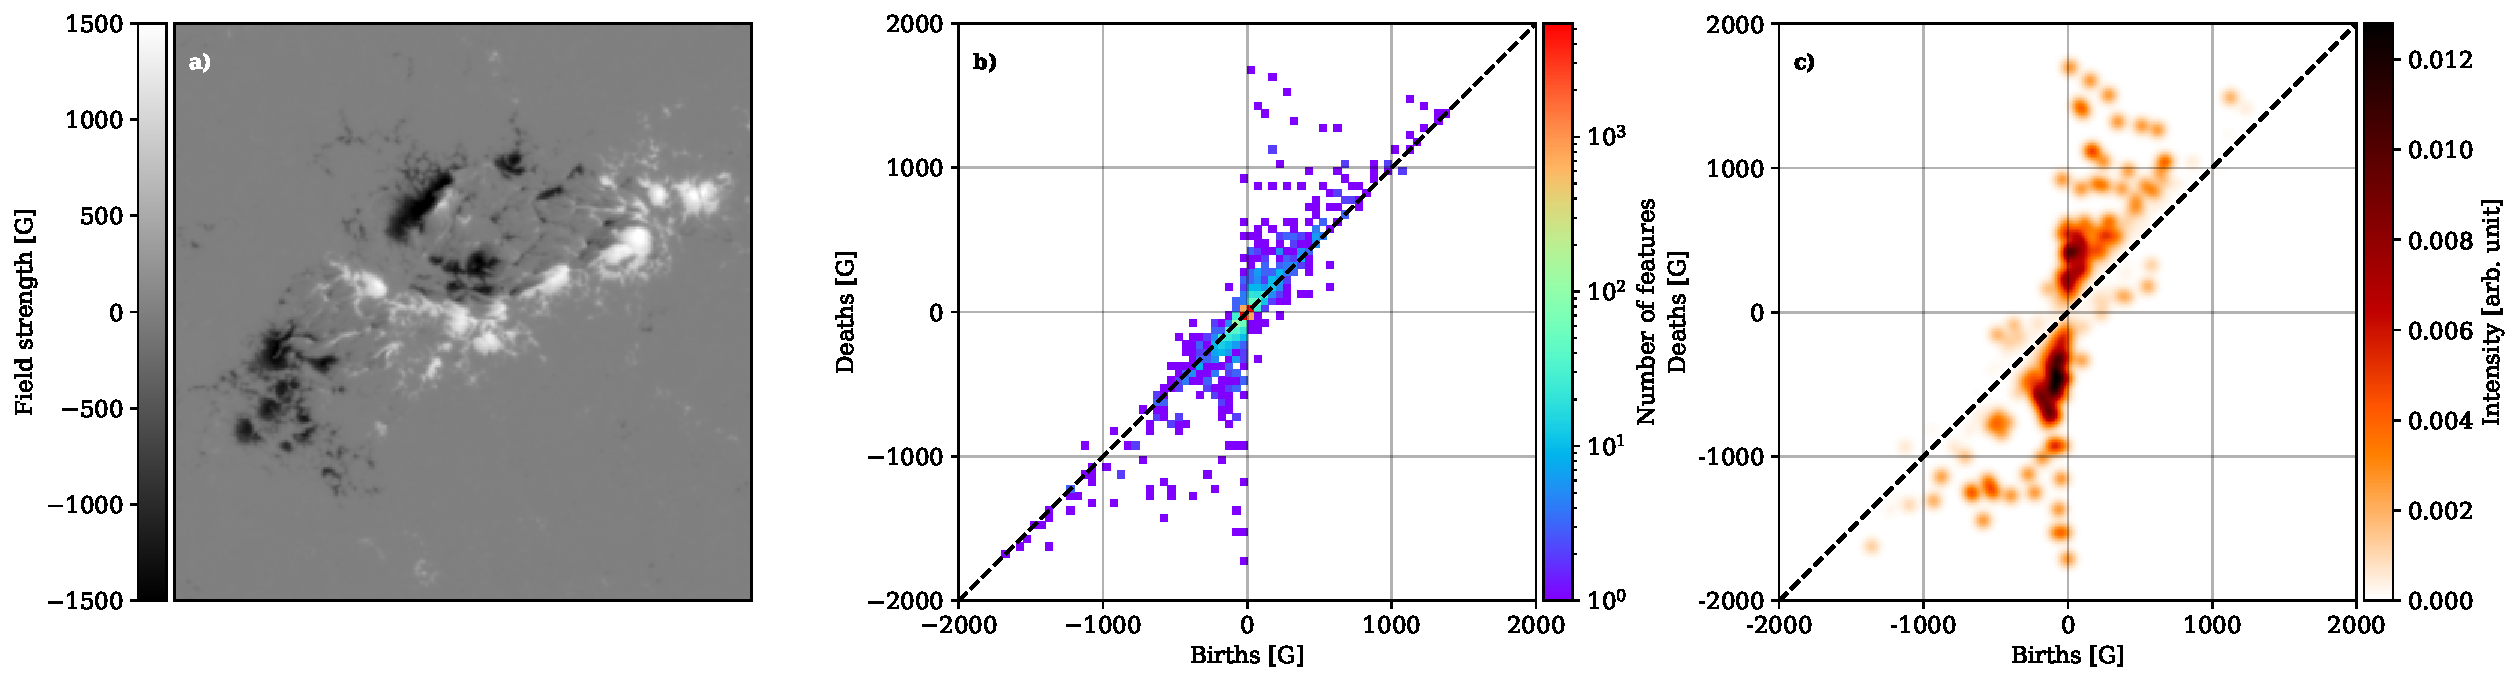
\includegraphics[width=\textwidth]{figures/PersistentHomology/PI_PD_example.pdf}
    \caption[Peristent diagram of an active region]{(a) SDO/HMI magnetogram taken on 2011-02-13 depicting an active region (NOAA AR 11158). (b) The corresponding PD combining superlevel and sublevel filtrations. (c) PI generated from the PD in panel b) with the following configuration: Resolution =  1000 pixels$^2$ ($4\ G$ per pixel), weighting function: $\omega (\pi) = \arctan (5\times 10 ^{-8} \pi ^{3})$ and a gaussian kernel with $\sigma = 40\ G$.}
   \label{fig: PD+PI_example}
\end{figure}


The application of persistent homology to a specific dataset can vary depending on the aims of the study. Different dimensions of the analysis and various types of filtrations focus on distinct features within the data. It is crucial to have prior knowledge of the expected structures and relevant features to be captured in the analysis in order to determine the appropriate approach. In this section, we aim to outline the most appropriate approach for studying the particular case of solar magnetograms.

The solar magnetograms employed here represent the longitudinal component of the magnetic field on the photosphere and are typically presented as greyscale images, as shown in Figure \ref{fig: PD+PI_example}, panel a). The polarity of the line-of-sight magnetic field is indicated by the sign of each pixel, where positive and negative signals correspond to field lines pointing towards and away from the observer. Applying a single filtration to a greyscale image only displays features corresponding to one polarity (positive or negative) in a PD. However, to conduct a comprehensive study of the magnetic field, both polarities are essential, thus necessitating the use of two separate filtrations with different filtration directions.

\begin{figure}[t]
    \centering
     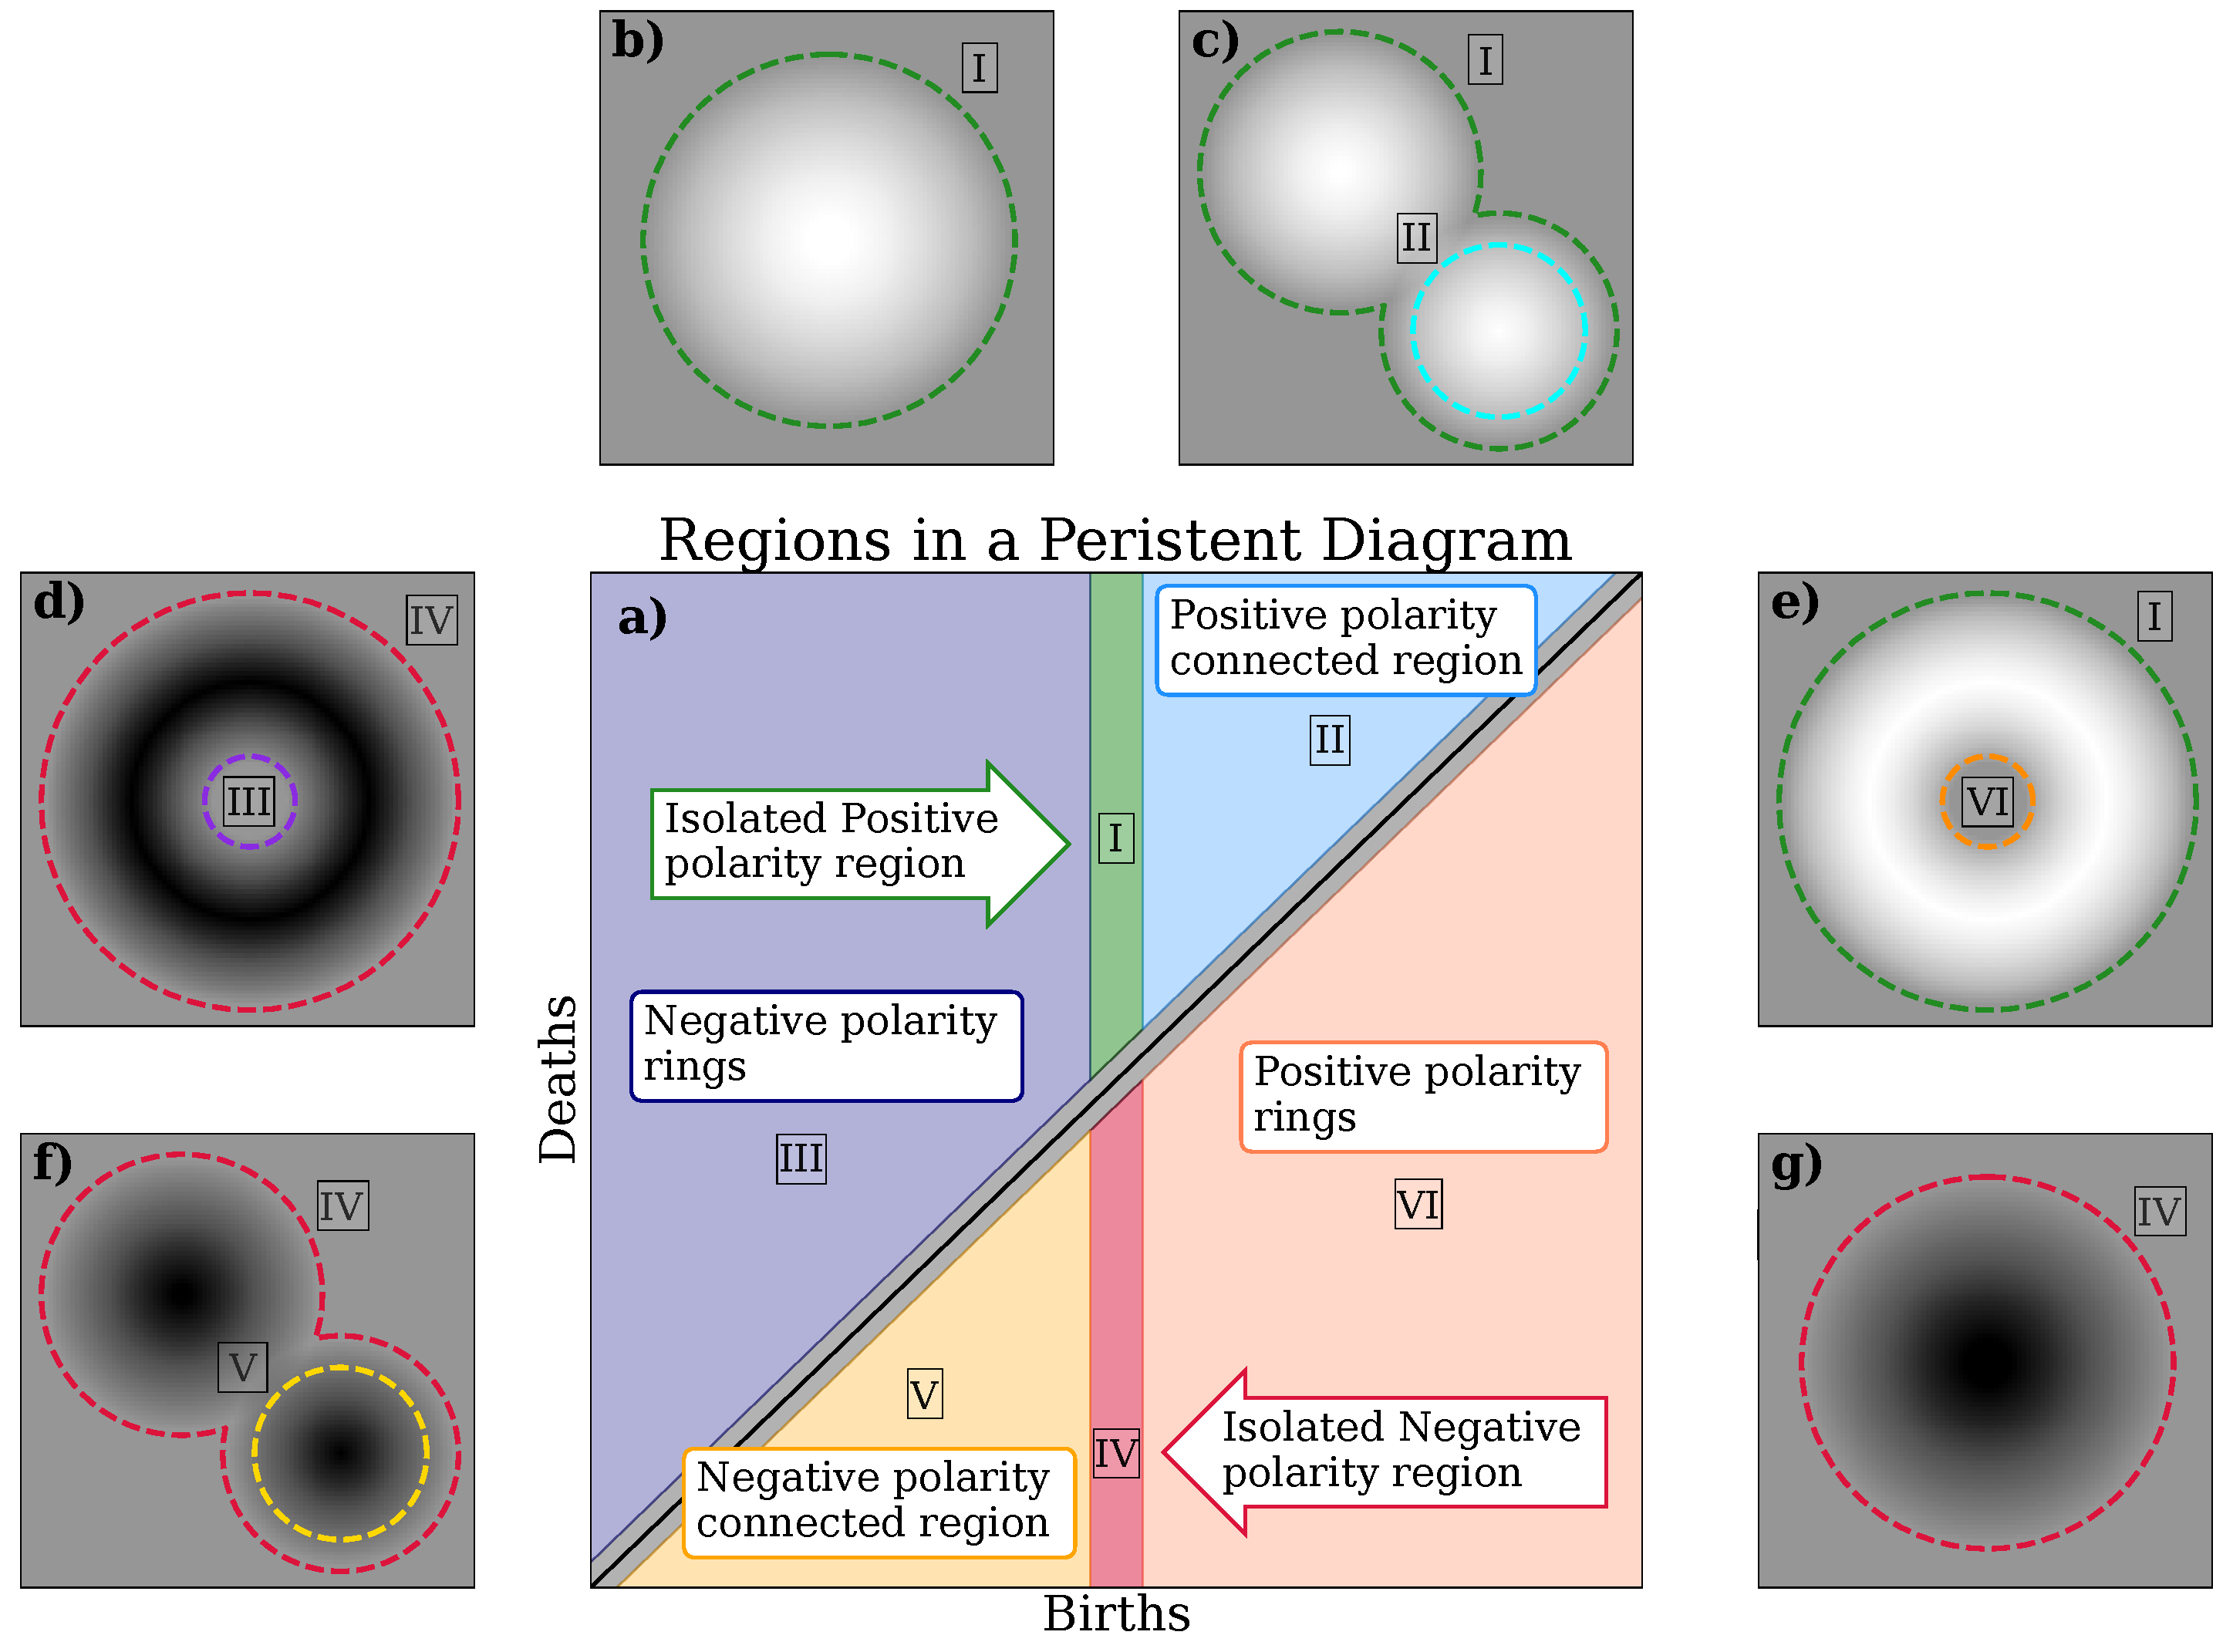
\includegraphics[width=12cm]{figures/PersistentHomology/Regions_anotated.pdf}
    \caption[Persistent diagram interpretation scheme.]{Schematic representation of the PD and the different regions (panel a)). The magnetic structures corresponding to the topological features found in the different regions are shown in panels b) to g), with each feature identified by a ring with the corresponding color.}
   \label{fig: PD REGIONS}
\end{figure}

We determined that a combination of superlevel and sublevel filtrations with a $1^{st}$-dimensional persistent homology analysis was the most suitable approach for studying solar magnetograms. This choice is based on two main reasons. Firstly, the $1^{st}$ dimensional analysis allows us to identify the most prominent features in a PD, which is not the case in the $0^{th}$ dimensional analysis where the strongest feature does not appear in the diagram as it never dies (see Fig.~\ref{fig_ph: Image Filtration Example}). Secondly, by combining superlevel and sublevel filtrations, we can display the results of both filtrations in a single diagram. Features corresponding to different filtrations will have persistencies with opposite signs (features found in a superlevel filtration will be born at higher filtration values than their death, resulting in a negative lifespan). This enables us to construct a PD in which all features displayed above the identity line (with positive persistencies) correspond to the sublevel filtration, and those below the line correspond to the superlevel filtration (see panel b) in Fig.~\ref{fig: PD+PI_example}).

The PDs, and consequently the PIs, offer valuable insights into the magnetic structures present in the magnetograms. The location of a topological feature on the diagram is completely determined by the properties of the corresponding magnetic structure. Specifically, this position is influenced by factors such as the maximum intensity of the magnetic field, its proximity to other magnetic structures, and its geometric shape, including the presence of holes or pores within the structure. These characteristics allow us to partition the diagram into distinct regions, where topological features within each region correspond to different types of magnetic structures.


We distinguished between six distinct regions in the diagram. Figure \ref{fig: PD REGIONS} illustrates these regions in panel a) and provides schematic representations of the corresponding magnetic structures in panels b) to g). The regions are as follows: first, topological features located above the identity line (positive persistencies) with birth values close to 0 (region I in the diagram). Features within this region represent isolated magnetic structures of positive polarity, that is, patches of positive magnetic flux fully enclosed by an absence of any magnetic field. The threshold defining what is considered ``close to 0$"$ is determined by the data's properties. To identify isolated structures, we set the threshold as a function of the statistical properties of the background signal (i.e. areas of the magnetogram with little magnetic flux). Specifically, the limits for this region are set as $(-5 \sigma _ {bg}, 5 \sigma _ {bg})$, where $\sigma _ {bg}$ denotes the standard deviation of the background signal found in a $15\times 15$ pixels box devoid of strong magnetic structures.

The second region (II in the diagram) comprises features above the identity line with positive birth values, representing connected structures with positive polarities, that is, positive magnetic field structures in contact with another positive structure but not fully merged. The third region (region III) contains topological features above the identity line with negative birth values, which corresponds to magnetic structures of negative polarity exhibiting a ring-like attribute, namely, structures with pores or holes. These three regions of the diagram have counterparts with negative persistencies. Thus, features associated with isolated structures of negative polarities are found in the region with a birth value close to 0 but below the identity line (region IV), features for connected negative structures are also located below the line but with negative birth values (region V). Lastly, features arising from positive magnetic structures with ring-like attributes are found below the identity line but with positive birth values (region VI).

\subsubsection{Quiet Sun results}


\begin{figure*}
    \centering
    {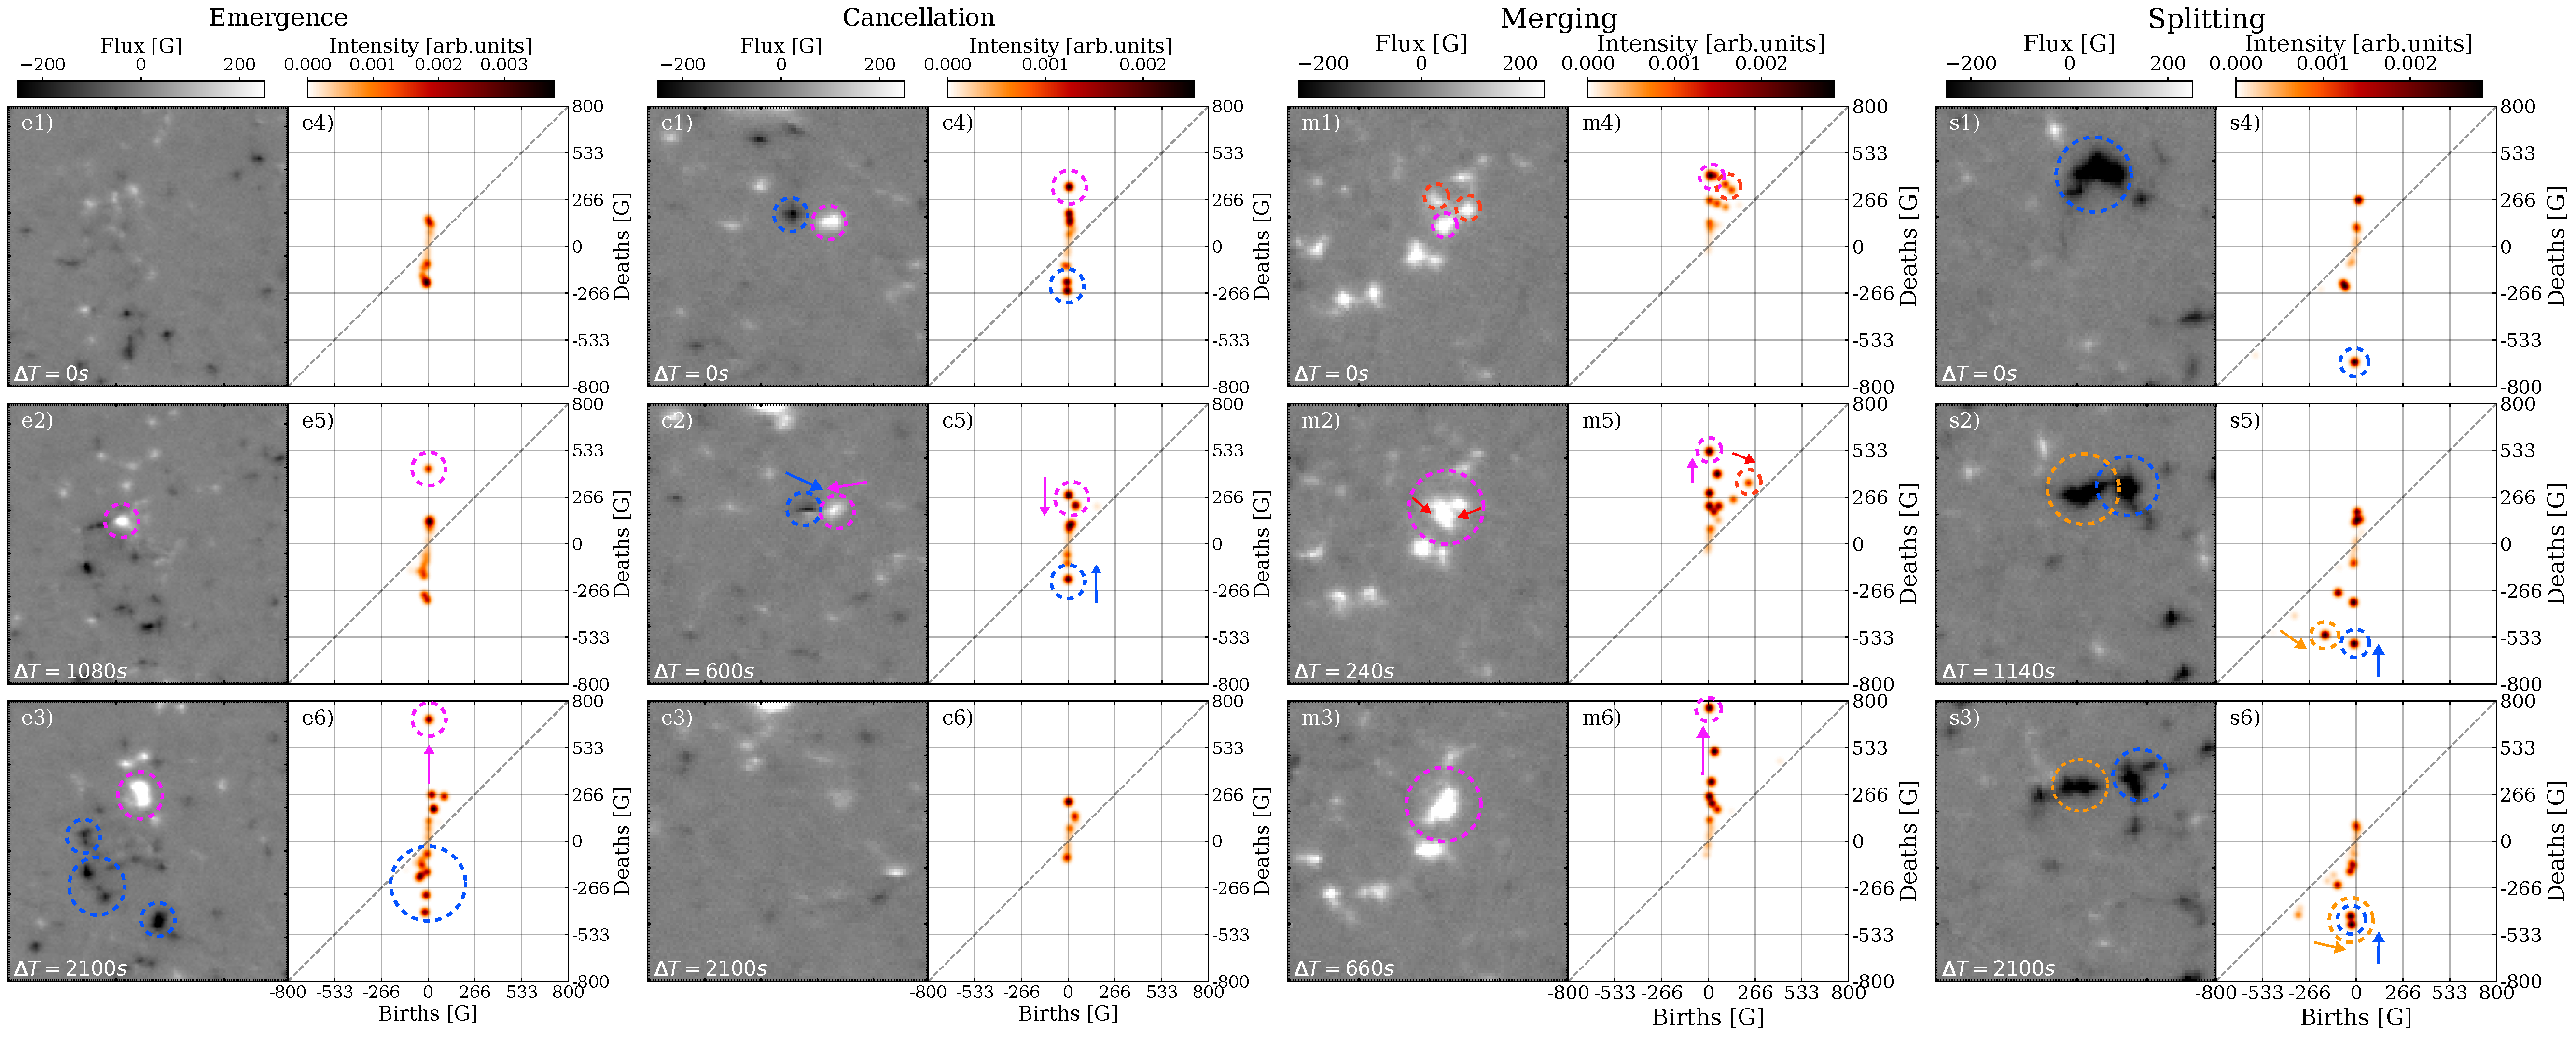
\includegraphics[width=15cm]{figures/PersistentHomology/QuietSun.pdf}}
    \caption[Opposite polarity interaction through persistent images.]{Examples of flux emergence (left column), flux cancellation (central left column), merging (central right column), and splitting (right column) events in the quiet sun. The time interval shown in the magnetograms is always with respect to the first frame (panel a) for emergence and g) for cancellation). The PIs correspond to the magnetogram to their left. The parameters for their computation are: resolution =  1000 pixels$^2$ (1.6 G per pixel), weighting function: $\omega (\pi) = \arctan (5\times 10 ^{-7} \pi ^{3})$ and a Gaussian kernel with $\sigma = $16 G.}
   \label{fig: Quiet_sun_events}
\end{figure*}

Quiet Sun regions are characterized by the presence of weak, small-scale magnetic field signals that exhibit rapid evolution. This rapid evolution leads to a multitude of signals in a single snapshot that evolve quickly from one frame to another. The small scale and rapid changes of the processes of the quiet Sun make data analysis techniques desirable for their study due to the complexity of such endeavors. 

When examining the evolution of signals across the entire field of view, we observe a dynamic process characterized by numerous regions interacting destructively while new signals emerge throughout the whole region. Despite these continuous changes, the overall structure of the magnetogram appears stable, with consecutive snapshots exhibiting strikingly similar properties. This apparent equilibrium state is also evident when studying the PIs, as consecutive frames show minimal differences in their representations.

Due to the apparent equilibrium state of the overall structure of the magnetograms, it is necessary to narrow down the field to which we apply the analysis. We found that when the number of signals in the studied region is lower, we can observe flux cancellation and emergence events, as well as merging and splitting events, through the changes induced in the persistence diagram. In cancellation events, two regions of magnetic flux with opposite polarities interact destructively, nullifying each other. On the contrary, in flux emergence events, we observe signals of both polarities suddenly emerge from a region with little magnetic flux. In splitting and merging events, only one polarity is involved. Two or more distinct structures of equal polarity merge together in merging events, and a single structure is divided into two or more for splitting events.

In Figure \ref{fig: Quiet_sun_events}, an example of an emergence event is shown in three snapshots through the magnetograms (panels e1 to e3) and their corresponding PIs (panels e4 to e6). When we focus on the second snapshot (panel e2 and e5), we see that a new positive and isolated feature (birth $\sim 0$) that was not present in the previous snapshot has appeared in the PI and stands out from the rest of the signals (highlighted with a pink circle in both magnetogram and PI), while simultaneously, the density of negative polarity features also begins to increase. In the last frame, we see that in the case of positive polarity, the majority of the signal has concentrated in a single structure, as shown by the increase of the death value of the corresponding feature in the PI. A few connected features are also seen, but these are less significant. Meanwhile, the negative polarity signal has been distributed into multiple structures instead of concentrating in a single one, as evidenced by the absence of a prominent feature in the PI and the increased density of connected features (highlighted with blue circles both in the PI and the magnetogram).

A very similar analysis can be carried out to analyze cancellation events. The evolution of the persistence image is very similar to that of the emergence events but in the opposite direction. Figure \ref{fig: Quiet_sun_events} also shows an example of a flux cancellation event through magnetograms (panels c1 to c3) and PIs (panels c4 to c6). In the beginning, the PI shows the presence of features of opposite polarities. When the corresponding structures approach each other and begin to interact, the magnetic signal starts to decrease, which is observed in the PI as a simultaneous movement of the features towards the center of the diagram. This reduction in signal continues until both features reach the center of the diagram, which corresponds to the moment when they will have completely canceled each other out (panels c3 and c6). 

For the events that only involve one polarity, namely merging and splitting events, the same behavior is seen in the PI for positive and negative features, but on their respective sides of the PI.

An example of a merging event of positive polarity structures is shown in Fig.~\ref{fig: Quiet_sun_events}, in panels m1) to m6). These events start with multiple isolated, or interacting structures (as shown in panels m1 and m4), that are moving towards each other. As the structures cluster, two movements are seen in the PI: firstly, the features corresponding to the structures with the weakest field (red features in panels m2 and m5) move towards the identity line; and secondly, the feature corresponding to the main structure (pink feature in panels m2 and m5) experiences an increase in its absolute death value due to the increase in magnetic flux coming from the rest of the structures. When the structures are fully merged, only a single feature appears in both the magnetogram and PI (pink feature in panels m3 and m6), in the isolated region (region I or IV, depending on the polarity).

This process is reversed for splitting events, as shown in panels s1) to s6) of Fig.~\ref{fig: Quiet_sun_events}. We see how an initially isolated feature in the PI (blue feature in panels s1 and s4) evolves into two (or multiple) features. When the process has started, but the two parts have not yet completely separated, a second feature appears in the diagram in the region corresponding to the connected structures (regions III or V in the diagram), as shown in panels s2) and s5). As the two structures continue to separate, this second feature gradually approaches the region for isolated structures (regions I and IV)  as the magnetic field surrounding it in the magnetogram diminishes (panel s5). Eventually, when both structures are completely separated (i.e. with no signal around them), they will both appear on the diagram as two isolated features with a lower death value compared to the initial one (panels s3 and s5). This reduction occurs because the magnetic flux is distributed between the two structures.

\subsubsection{Active region results}

\begin{figure}
    \centering
    {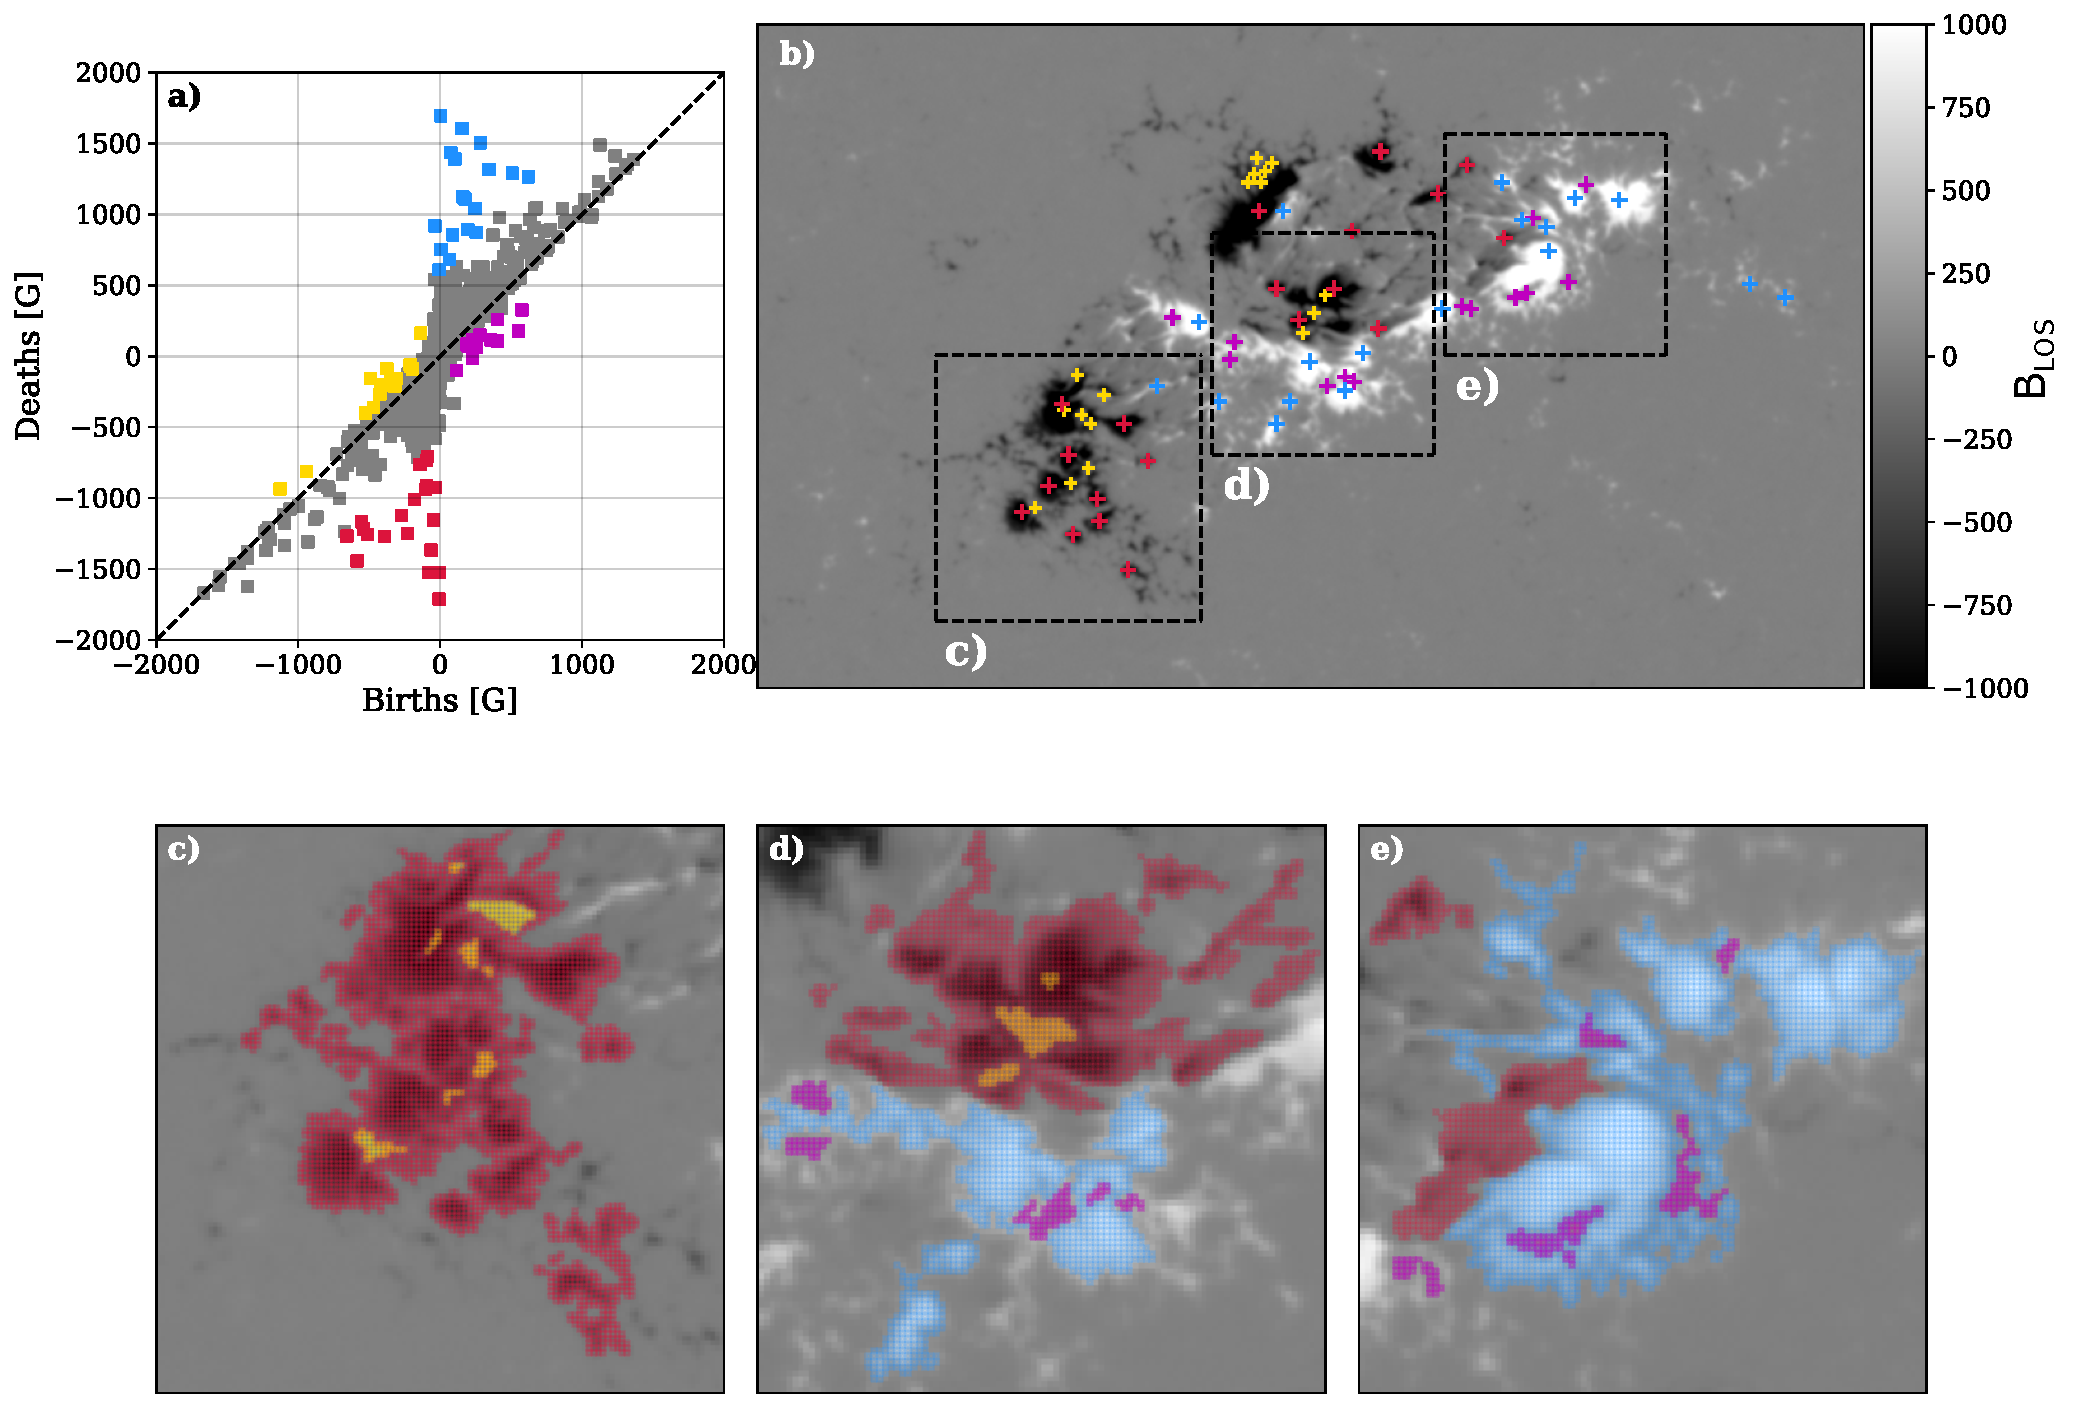
\includegraphics[width=15cm]{figures/PersistentHomology/AR_analysis_v2.pdf}}
    \caption[Feature detection in active regions through persistent diagrams.]{SDO/HMI magnetogram taken on 2011-02-13 at 06:34 UT depicting an active region (NOAA AR 11158) and the corresponding persistent diagram (panel a)). Panels c) to e) display a zoomed region of the active region, corresponding to the labeled region with the same letter in panel b). Features of different types are shown in different colors in the diagram. The corresponding structures are shown in the same colors in the magnetograms; as colored crosses in panel b) and as a colored transparent overlay displayed over the whole pixel in panels c) to e) to show the extent of the structure.}
   \label{fig:  AR - Complexity}
\end{figure}

It is important to understand which types of magnetic structures can be identified through persistent homology and establish the correspondence between these structures and the position of the corresponding topological feature in a persistence diagram. To achieve this understanding, Fig. \ref{fig:  AR - Complexity} displays both a magnetogram with complex morphology (panel b) and its corresponding persistence diagram (panel a), along with three zoomed-in regions of the magnetogram (panels c to e). In all panels, some topological features or their corresponding magnetic structures have been color-coded based on their types, or equivalently, based on their positions in the persistence diagram. In the complete magnetogram (panel b), structures have been marked with a cross, indicating the pixel where the structure died during the filtration process. Meanwhile, in panels c to e, all pixels composing each structure have been colored. It is noteworthy that nearly all pixels appear colored because we have selected the most significant structures—those with longer lifetimes (Eqn. \eqref{eq: persistence}). Consequently, these structures encompass all less significant structures that are absorbed and incorporated into the former during the filtration process.

The analysis of the persistence diagram allows us to deduce several properties of the magnetogram. Firstly, the persistence diagram provides a rapid assessment of the intensity of the magnetic flux since the death value of the topological feature coincides with the maximum flux (in absolute value) within the corresponding structure. In the case of Figure \ref{fig:  AR - Complexity}, we observe that several structures exhibit maximum (absolute) values surpassing 1500 G, with multiple structures falling within the range of 1000 G to 1500 G.

Secondly, we can infer how the magnetic signals are distributed by examining the number of isolated and connected structures in the diagram (structures highlighted in blue and red depending on their polarity in Fig. \ref{fig:  AR - Complexity}). The complex morphology of the structure displayed in the magnetogram is evident in the high number of connected structures (regions II and V in the diagram) and the absence of prominent isolated structures (regions I and IV).

Lastly, the presence or absence of ring-like structures provides insights into how the magnetic structures are connected. These features can only be found in regions where connected structures create highly complex morphologies with gaps between them, as illustrated in the magnified regions of the magnetogram in Figure \ref{fig:  AR - Complexity} (panels c to e).

An example of how the three features allow us to classify ARs depending on their morphologies is shown in Figure \ref{fig: AR-classification}, where three different ARs and their corresponding PIs are displayed. Although at first sight, the PIs appear to be very similar, especially the ones shown in panels d) and f), upon closer inspection, it is possible to find the differences when focusing on the three features mentioned previously. The first AR (panel a)), also shown in Fig. ~\ref{fig:  AR - Complexity}, shows a very complex morphology, where the magnetic field of both positive and negative polarities is distributed in multiple connected structures. This behavior is displayed in the PI through the high density in the isolated and connected features in equal proportions (i.e. with no prominent features) and with the presence of ring-like features in both polarities. In contrast, the second AR (panel b) shows a simpler magnetic structure with weaker signals. The PI for this case shows an absence of ring-like features in both polarities and a very low density in the regions for connected and isolated features. Lastly, panel c) shows an AR where the positive magnetic field is concentrated in one main area whereas the negative polarity magnetic field shows a fragmented structure. Comparing the corresponding PI with that of the initial case (panels f and d, respectively), a similarity is evident in the region corresponding to negative polarities, observed in both the density of connected components and the presence of ring-type structures. Nevertheless, when examining the positive polarity, it becomes evident that, unlike its negative counterpart, there are only a few prominent isolated structures and a notably low density of connected structures. Furthermore, this asymmetry between the positive and negative distributions is underscored by the absence of ring-like structures in the former.

\begin{figure}[t]
    \centering
     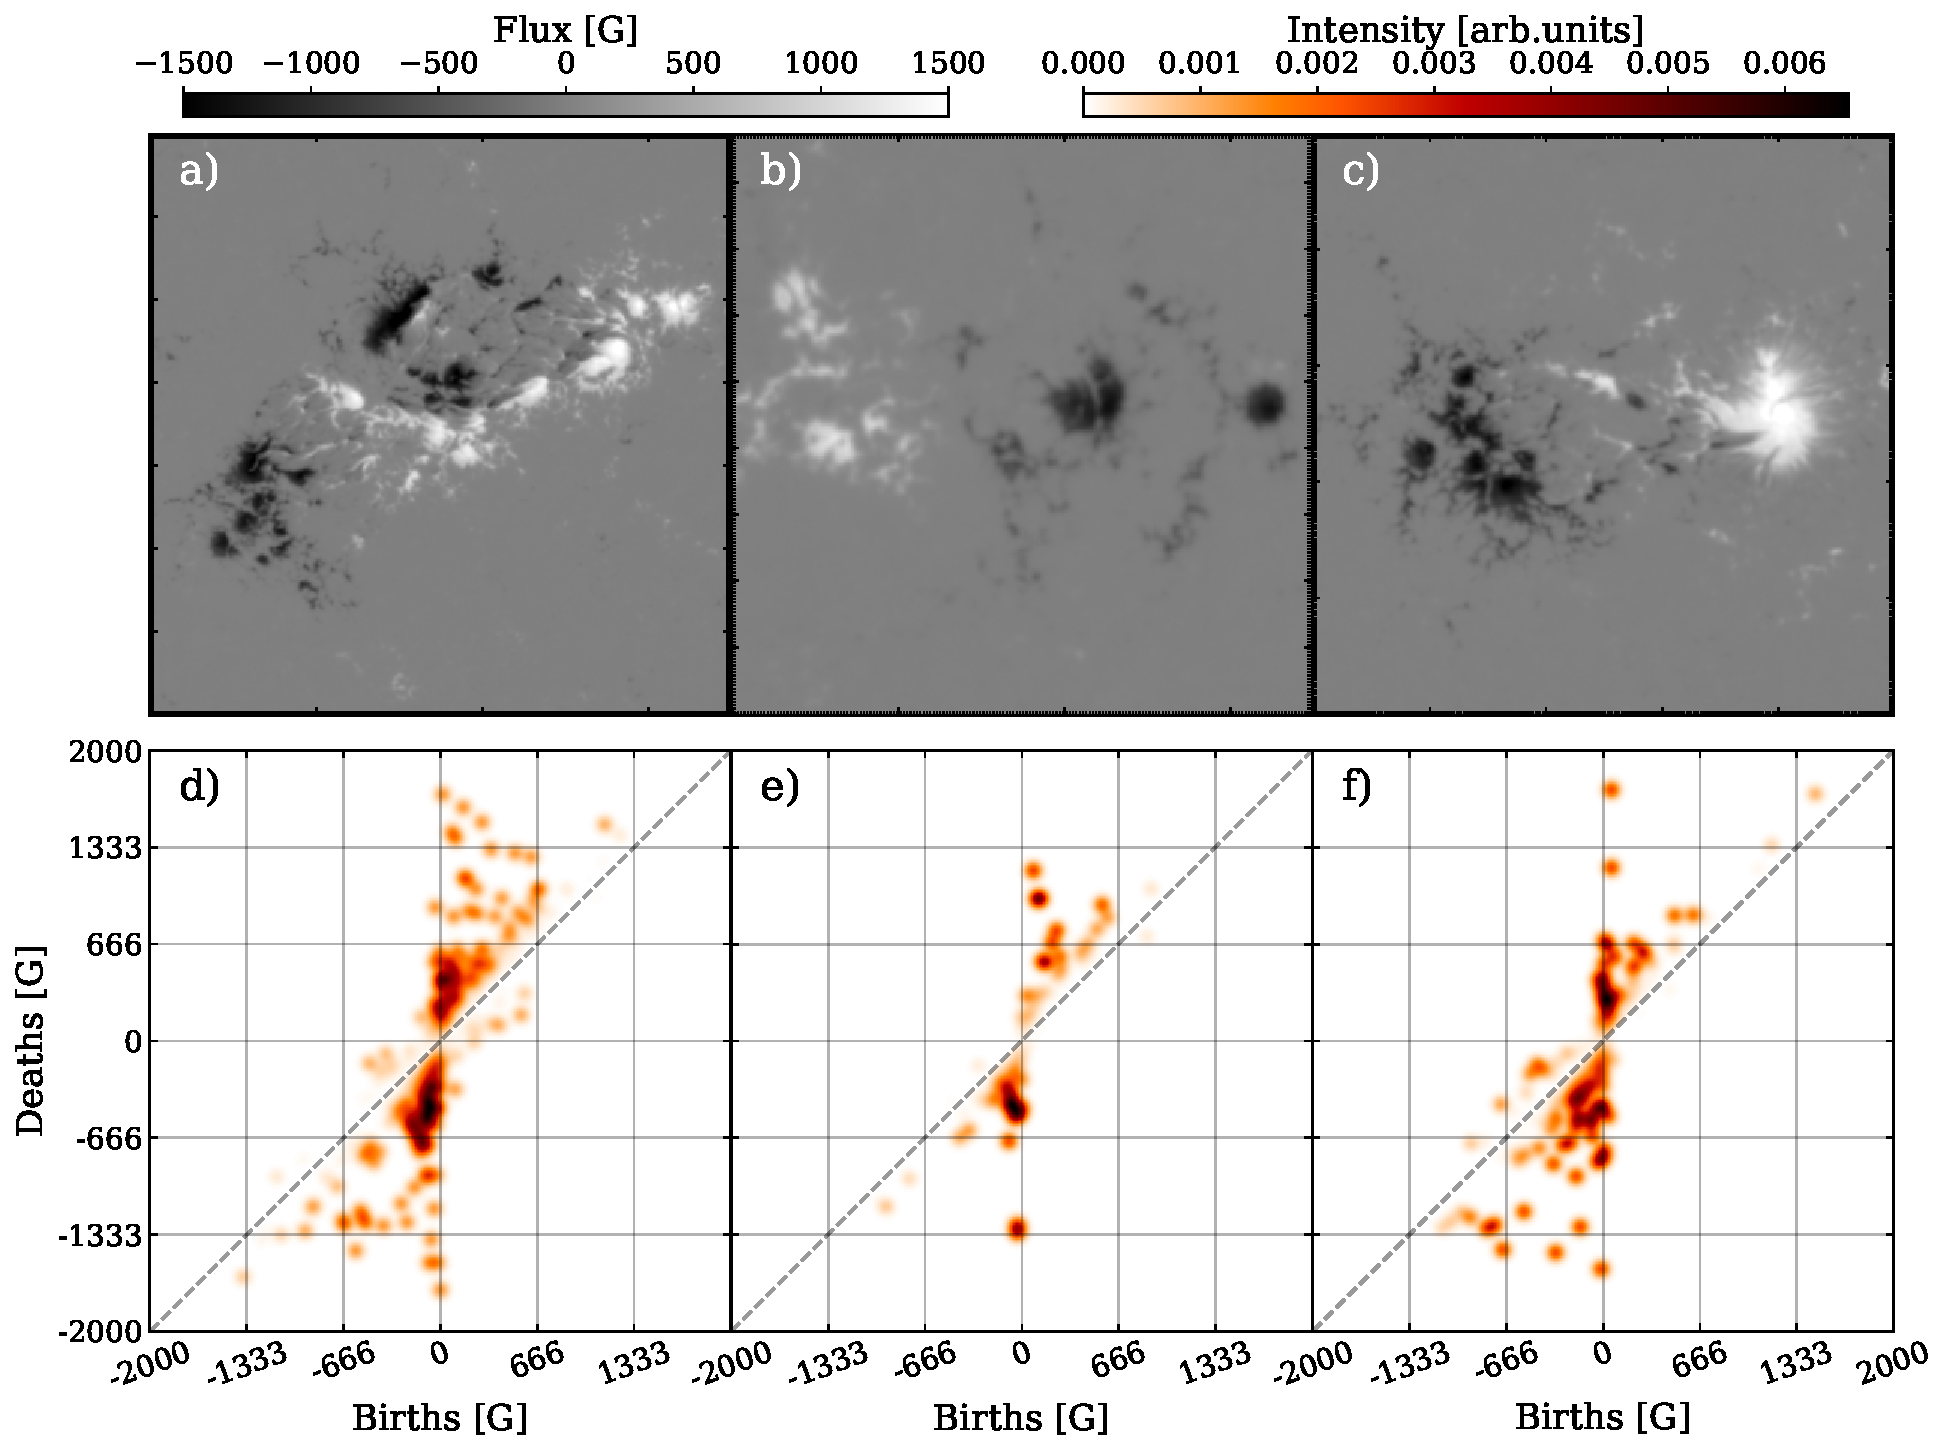
\includegraphics[width=15cm]{figures/PersistentHomology/AR_classification.pdf}
    \caption[Morphology of persistent images.]{SDO/HMI magnetograms of three different active regions and their corresponding persistence images. a) NOAA AR 11158, date: 2011-02-13 at 06:34. b) NOAA AR 11098, date: 2010-08-12 at 20:58. c) NOAA AR 11072, date: 2010-05-22 at 20:58. All persistence images have been generated with the following parameters: Resolution =  1000 pixels$^2$ (4 G), weighting function: $\omega (\pi) = \arctan (5\times 10 ^{-8} \pi ^{3})$ and a gaussian kernel with $\sigma = 40\ G$.}
   \label{fig: AR-classification}
\end{figure}

\subsubsection{`Interacting' Diagram}

So far, we have shown how persistent homology is capable of identifying the various morphologies of active regions and the types of structures that can be identified through persistent images or diagrams. Nevertheless, these structures are either isolated or regions of the same polarity that interact with each other. Due to the nature of the filtration process, persistent homology is unable to detect structures where magnetic fields of opposite polarities form a joint structure. However, ARs where there is a significant interaction between magnetic fields of opposite polarities are of greater interest due to their association with flare production. 

This issue is illustrated in the analysis carried out in the previous section of NOAA Active Region 11158 (see Fig. ~\ref{fig:  AR - Complexity}). Although we can capture the complexity of both positive and negative magnetic structures through the persistent diagram, the $\delta$-spots present in the central region remain unnoticed. However, the large number of flare events associated with this region including an X2.2-class event are thought to be related to the abundance of these structures (e.g. \citealt{x21}, \citealt{x22}). In this section, we describe a way to efficiently detect and quantify these structures using persistence homology, with only a few additional steps in the analysis.

%\begin{figure}
    %\centering
    %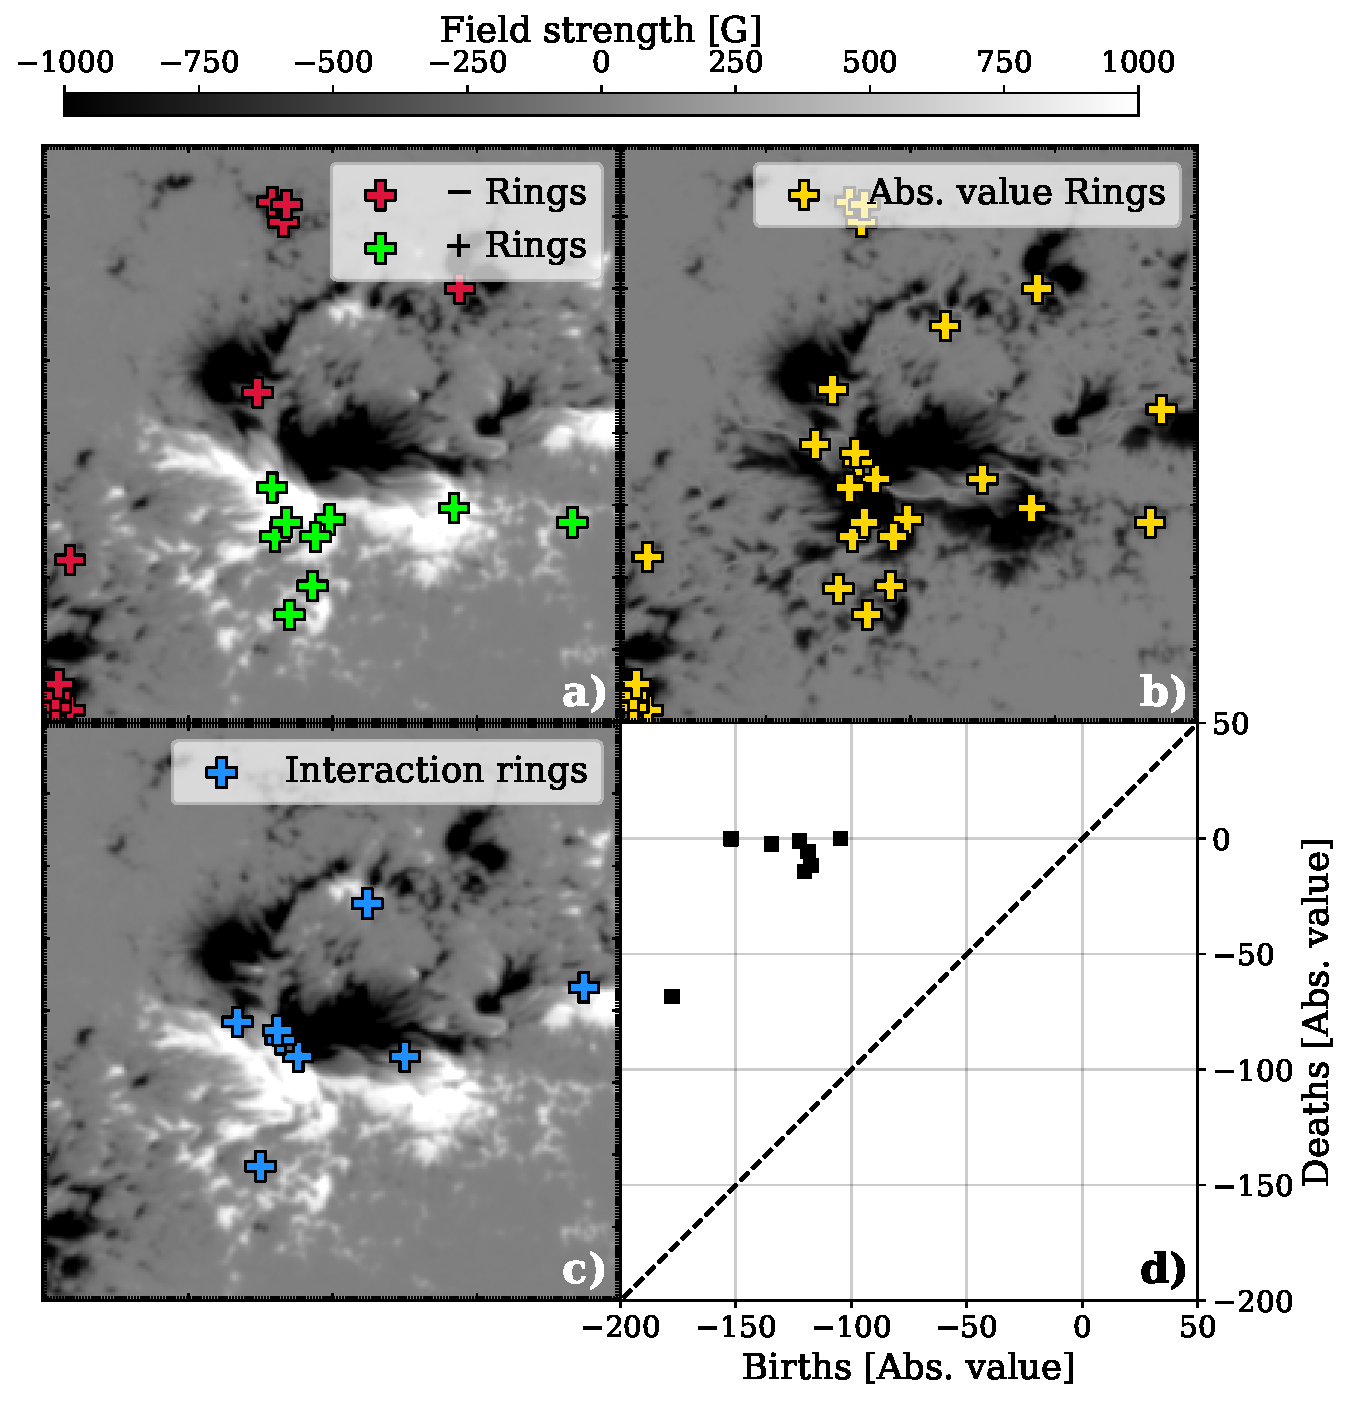
\includegraphics[width=8cm]{figures/PersistentHomology/InteractingDiagram.pdf}
   % \caption{
   %Depiction of the different steps carried out for the %generation of the interaction diagram (panel d)) for a %zoomed-in region of an SDO/HMI magnetogram of NOAA AR %11158 observed on the 2011-02-13 at 18:34. The crosses %point to the position at which each of the ring-like %structures die, which is always located inside the %perimeter of the hole. Panel a) shows the original %magnetogram and the position where rings of positive and %negative polarities are found. Panel b) shows the %magnitude of the field strength in negative values along %with the rings found in this representation. Panel c) %shows the original magnetogram again, but now featuring %the interaction rings, identified when comparing the %position of the rings found in the previous steps. %Lastly, panel d) shows the `interaction diagram' %generated using only the interacting ring structures.}
 %   \label{fig: Interacting_diagram}
%\end{figure}

\begin{figure}
  \begin{minipage}[c]{0.5\textwidth}
    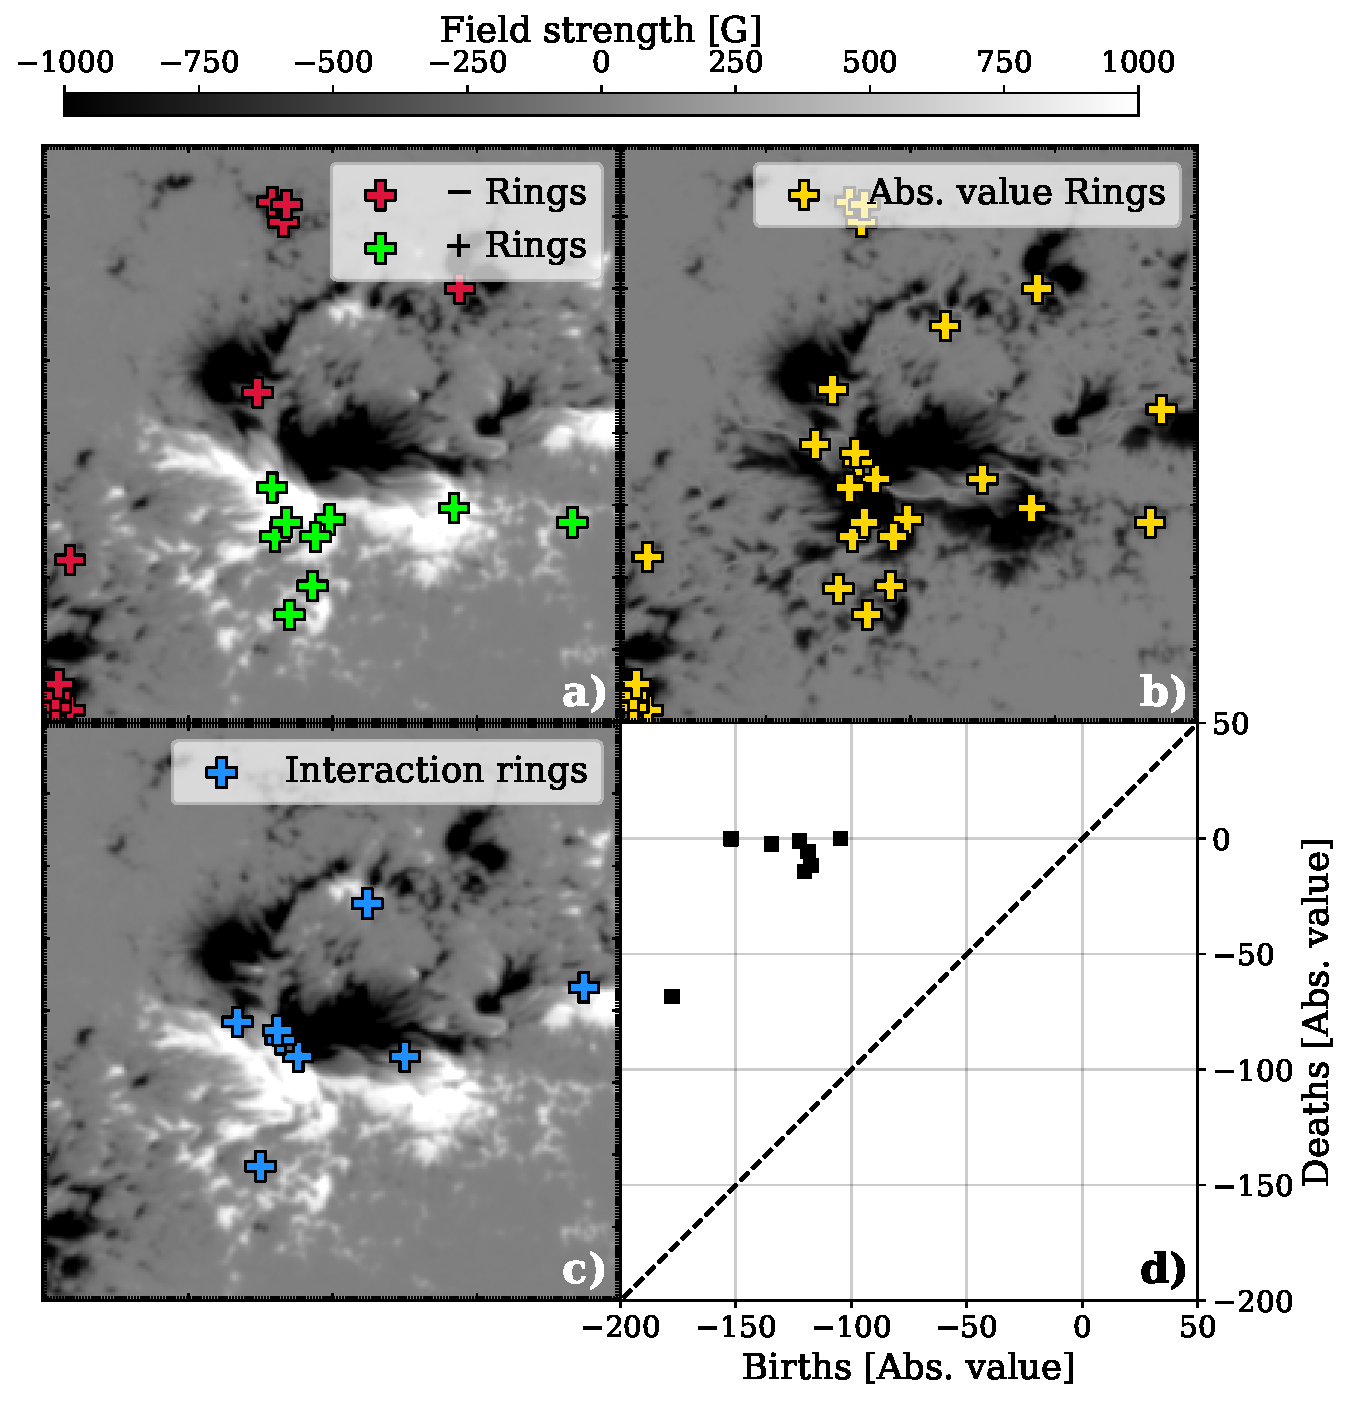
\includegraphics[width=\textwidth]{figures/PersistentHomology/InteractingDiagram.pdf}
  \end{minipage}\hfill
  \begin{minipage}[c]{0.5\textwidth}
    \caption[Interaction diagram]{
      Depiction of the different steps carried out for the generation of the interaction diagram (panel d)) for a zoomed-in region of an SDO/HMI magnetogram of NOAA AR 11158 observed on the 2011-02-13 at 18:34. The crosses point to the position at which each of the ring-like structures die, which is always located inside the perimeter of the hole. Panel a) shows the original magnetogram and the position where rings of positive and negative polarities are found. Panel b) shows the magnitude of the field strength in negative values along with the rings found in this representation. Panel c) shows the original magnetogram again, but now featuring the interaction rings, identified when comparing the position of the rings found in the previous steps. Lastly, panel d) shows the `interaction diagram' generated using only the interacting ring structures.
    } \label{fig: Interacting_diagram}
  \end{minipage}
\end{figure}

We start by tracking the position in the magnetogram where rings are detected. Following this, we modify the magnetogram by inverting the sign of one polarity, ensuring that all pixels are either negative or positive. This way, we construct a second `magnetogram' in which we only have information about the intensity, in absolute value, of the LOS magnetic field. This allows us to identify features formed by any combination of signals, whether they are of the same polarity or opposite. Using this new magnetogram, we repeat the analysis and record the positions in the magnetograms at which we find ring-like features. It is worth noting that in this analysis, all the rings identified in the initial step, which were formed by structures of equal polarities, are still detected, although their position in the persistent diagram may have changed due to the change in polarity, hence the relevance of tracking the pixel in the magnetograms. However, only in this second analysis can we identify rings formed between opposite polarities. By selectively considering the ring-like features exclusively identified in this second analysis, we can effectively identify and characterize the structures that are formed by the interaction between different polarities. 

Figure \ref{fig: Interacting_diagram} depicts an example of the interaction analysis for NOAA AR 11158, which exhibits a strong interaction between opposite-polarity fields. Panel a) displays the magnetogram, indicating also the positions where ring-like features have been identified for both positive and negative polarities. Only features with absolute persistencies greater than $5\sigma _ {bg}$ and whose birth occurs in the range: ($5\sigma _ {bg}, \infty$), for positive polarities, and: ($-\infty, -5\sigma _ {bg}$) for negative polarities, have been recorded. We now repeat the same analysis but using only the magnitude of the signal. To do this, we invert the positive polarity and, once again, register the positions of the ring-like features in this new magnetogram, as shown in panel b). As observed in panel c), the majority of the interaction rings (\textit{i.e.} those exclusively identified in the second analysis) are located in areas characterized by strong interaction, where the $\delta$-spots were found. In these areas, both polarities interact, resulting in the formation of ring-like structures comprising positive and negative magnetic fields due to their close proximity. These areas, such as  $\delta$-spots, are of particular interest, as they typically harbor magnetic cancellation, reconnection, and flux emergence.  However, some points appear to be situated in uni-polar fields. These points, despite what may appear at first sight, are found by this analysis due to a structure that requires the other polarity to close completely and thus form a ring. It is noteworthy that the occurrences of such cases are quite limited when compared to the rings observed in highly interacting zones. While their presence does not necessarily indicate intense interaction, it does imply a certain level of interaction between the two polarities. These features can be represented in a persistence diagram in an analogous way to the standard results of a persistent homology analysis. This is what we have referred to as `interacting diagram' and it is worth noting that only the magnitude of the birth and death coordinates are relevant parameters since the sign will be the one matching the polarity selected at the second step. We have chosen to invert the positive polarity so that these features have positive persistencies, as it is more common in persistent homology studies. However, it is important to emphasize that this decision is completely arbitrary and has no impact on the results of the analysis.  

It is useful to determine the information conveyed by the interaction diagram regarding the structures themselves. By taking into account the position and quantity of the interaction rings, along with the temporal evolution of the diagram, we can discern the moment and location where these highly interacting structures develop. Therefore, interaction diagrams could be a new tool to identify, through their topological properties, the strong-gradient polarity inversion lines that characterize $\delta$-spots. To achieve this, it is necessary to incorporate into the analysis the temporal evolution of these structures and study the properties that can be extracted from the $\delta$-spots through these diagrams, which goes beyond the scope of this work but represents the next (necessary) step to asses the predicting capabilities of persistent homology in the field of solar physics.




%\chapter{Summary and conclusions}
%The conclusions are \dots

%\appendix
%\chapter{Profile derivatvies}

\bibliography{bibliography}

\cleardoublepage
\layout

\end{document}